\documentclass[dutch,a4paper,12pt,doubleside]{book}

\usepackage[T1]{fontenc}
\usepackage[dutch]{babel}
\usepackage[utf8]{inputenc}
\usepackage[margin=3cm]{geometry}
\usepackage{amsthm}
\usepackage{hyperref}
\usepackage{minted}
\usepackage{float}
\usepackage{trimspaces}
\usepackage[nottoc]{tocbibind}
\usepackage[labelfont=bf]{caption}
\usepackage{tabularx}
\usepackage{array}
\usepackage{dirtree}

% headers and footers (page numbering)
\usepackage{fancyhdr}
\fancyhf{} % clear all header and footers
\renewcommand{\headrulewidth}{0pt} % remove the header rule
\fancyfoot[R]{\thepage} % Left side on Even pages; Right side on Odd pages
\pagestyle{fancy}
\fancypagestyle{plain}{%
  \fancyhf{}%
  \renewcommand{\headrulewidth}{0pt}%
  \fancyhf[lef,rof]{\thepage}%
}

% Card suits
\DeclareSymbolFont{extraup}{U}{zavm}{m}{n}
\DeclareMathSymbol{\varheart}{\mathalpha}{extraup}{86}
\DeclareMathSymbol{\vardiamond}{\mathalpha}{extraup}{87}

\usepackage{makeidx}
\usepackage{hyperref}
\usepackage{minted}

% New line per paragraph, instead of indentation
\usepackage[parfill]{parskip}

% Prevent balancing vertical alignment
\raggedbottom

% Sets global font
\usepackage{tgpagella}

% Font utility function
\newcommand{\fon}[1]{\fontfamily{#1}\selectfont}

\usepackage[table, x11names]{xcolor}
\definecolor{blue}{RGB}{0, 149, 200}
\definecolor{green}{RGB}{0, 200, 136}

\captionsetup{justification=raggedright,width=.8\linewidth}

\usepackage[many]{tcolorbox}
\newtcolorbox{deftbox}{
    enhanced,
    sharp corners,
    frame hidden,
    boxrule=0em,
    left=1em,
    toptitle=1em,
    top=0.25em,
    bottom=1em,
    bottomtitle=0mm,
    colback=black!4,
    colbacktitle=black!4,
    coltitle=black!60,
    fonttitle=\bfseries\small,
    fontupper=\small,
    borderline west={2pt}{0pt}{black!20},
    grow to left by=-2em,
    grow to right by=-2em
}
\newtcolorbox{defbox}[1]{
    enhanced,
    sharp corners,
    frame hidden,
    boxrule=0em,
    left=1em,
    toptitle=1em,
    top=0.25em,
    bottom=1em,
    bottomtitle=0mm,
    colback=black!4,
    colbacktitle=black!4,
    coltitle=black!60,
    fonttitle=\bfseries\small,
    fontupper=\small,
    borderline west={2pt}{0pt}{black!20},
    grow to left by=-2em,
    grow to right by=-2em,
    title={#1}
}
\newtcolorbox{quotebox}{
    enhanced,
    sharp corners,
    frame hidden,
    left=1em,
    right=1em,
    top=1em,
    bottom=1em,
    colback=black!4!white,
    fontupper=\small,
    grow to left by=-2em,
    grow to right by=-2em
}

\def\trim#1{\ignorespaces#1\unskip}

\newcommand{\blockquote}[2]{
    \hfill
    \begin{quotebox}
    \begin{flushleft}
        ``\trim{#1}''
        \newline\newline\rightline{\textbf{-- \trim{#2}}}
    \end{flushleft}
    \end{quotebox}
    \noindent
}

\renewcommand{\listingscaption}{Codevoorbeeld}
\renewcommand{\listoflistingscaption}{Overzicht van codevoorbeelden}
\counterwithin{listing}{chapter}
% \usepackage[chapter]{minted}



\renewcommand\indexname{Trefwoorden}
\makeindex

\hypersetup{
  colorlinks,
  allcolors=[rgb]{0.3,0.3,0.8},
  linktoc=all
}

\title{BEP2 Reader}
\author{A. Rothuis}

\begin{document}

\maketitle

{\hypersetup{linkcolor=black}
\tableofcontents
}


\part{De cursus}
\chapter{Cursusopzet}
Tijdens de cursus \textbf{Backend Programming 2 (BEP2)} leren we 
een structureel kwalitatief hoogstaande back-end 
op te zetten aan de hand van bestaande oplossingen en standaarden.
Hoewel we een boel zullen herhalen, bouwt dit voort 
op de kennis en vaardigheden
die we bij \textbf{Object-Oriented Analysis (OOAD)}, 
\textbf{Object-Oriented Programming (OOP)}
en \textbf{Backend Programming 1 (BEP1)} hebben opgedaan.

Daarnaast is er samenhang met \textbf{Data en Persistency (DNP)}:
we maken gebruik van een  relationele database om langdurige 
opslag te verwezenlijken. Bij DnP wordt meer stilgestaan bij 
de onderliggende techniek, terwijl we bij BEP2 dankbaar gebruik 
maken van library en frameworks die een hoop werk uit handen halen.

Deze cursus bereid je voor op projecten en andere cursussen, zoals
\textbf{Continuous Integration and Software Quality (CISQ)} 
en \textbf{Software Architecture (SARCH)},
maar ook op je stages en je carrière. Hoewel we Java als taal gebruiken 
en Spring Boot als framework, zijn de ideeën namelijk
toepasbaar op heel veel andere programmeertalen en frameworks!
Let dus goed op als je binnenkort al wil starten als software developer.

De vraag die in deze cursus centraal staat is als volgt:

\begin{defbox}{Centrale vraag}
Hoe kunnen we een flexibele, onderhoudbare webapplicatie opzetten, waarin we bestaand werk kunnen hergebruiken?
\end{defbox}

\section{Kennisbasis}
Om deze centrale vraag te beantwoorden ontwikkelen we 
een web-applicatie met \textit{Spring Boot}, een veelgebruikt 
en modern Java-framework voor web development. Voor de persistentie 
gebruiken we \textit{PostgreSQL} tezamen met \textit{Spring JPA} dat
onderwater \textit{Hibernate} gebruikt als object-relational mapper.

We werken aan flexibele software door te letten
op een separation of concerns, loose coupling en high cohesion.
Daar kan een modulaire, gelaagde applicatiearchitectuur aan bijdragen.

Voor het ontwerp en de realisatie van onze software benutten we 
het objectmodel: object oriëntatie zoals het bedoeld is! 
Dit wordt aangevuld door een aantal design principles om tot een 
beter ontwerp te komen. We zetten polymorfisme en compositie in 
om via dependency injection de onderdelen binnen onze applicatie 
op flexibele wijze los te koppelen van elkaar.

In de realisatie van het project implementeren we een aantal
design patterns, een aantal standaardoplossingen voor 
veelvoorkomende problemen.

\newpage
\section{Leerdoelen}
Na deze cursus kan de student:
\begin{itemize}
    \item de structurele kwaliteit van software beoordelen aan de hand van de begrippen \textbf{separation of concerns}, \textbf{cohesion}, \textbf{coupling}
    \item de eigenschappen van object-orientatie, in de zin van het \textbf{objectmodel}, toepassen om onderhoudbare, object-georiënteerde software te ontwerpen en te realiseren
    \item \textbf{dependency injection} toepassen om flexibele, losgekoppelde software te verwezenlijken, waarvan de onderdelen te vervangen zijn
    \item \textbf{design principles} toepassen, zoals SOLID, om object-georiënteerde software te ontwerpen en realiseren
    \item \textbf{design patterns} herkennen en realiseren, zoals die van de Gang of Four, als abstracte standaardoplossingen om software te ontwerpen en te realiseren
    \item de \textbf{REST-principes} op de juiste wijze toepassen op een web applicatie
    \item een \textbf{web framework}, zoals Spring Boot, inzetten om een REST API te realiseren
    \item een \textbf{object-relational mapper (ORM)} tezamen met de \textbf{repository pattern} gebruiken, zoals met Spring Data JPA (Hibernate), om object-georiënteerde persistentie te realiseren
    \item werken binnen een \textbf{gelaagde architectuur}, waarbij elke laag ziet op één abstractieniveau en één soort logica
\end{itemize}

\section{Toetsing}
De leerdoelen worden getoetst aan de hand van een \textbf{individuele opdracht met interview}.
De criteria hiervoor zijn opgenomen op Canvas. 

Dit betekent dat de student gedurende de cursus een softwareproject realiseert.
Aan het eind van de cursus wordt een assessmentmoment ingepland. De student
presenteert zijn of haar werk en beantwoordt aan de hand van het project
vragen over de theorie. Ter voorbereiding is het verstandig om de theorie al 
een beetje in de presentatie op te nemen, 
bijvoorbeeld middels een korte PowerPoint-presentatie.

Studenten hebben laten zien dat het goed mogelijk is om een mooi cijfer te halen 
door naar deze criteria te kijken, de colleges bij te wonen en tijdens de cursus 
feedback te vragen en te verwerken. Het loont om daar de tijd voor te nemen.

\subsection{Studiebelasting}
Voor deze cursus staat een studie belasting van 5 ECs (European Credits). 
In Nederland wordt dit gelijkgesteld met 140 uur inclusief colleges.
De opdracht is echter zo ontworpen dat er voldoende ruimte is.
Zo kan je weggezakte kennis ophalen, zaken opzoeken en uitproberen
en feedback verwerken.

Het loont om een weekplanning te maken om regelmatig aan de opdracht 
te werken. Tijdens het programmeren zelf kan je een stuk sneller werken door 
gebruik te maken van alle shortcuts en functionaliteiten die je 
IDE (bij voorkeur IntelliJ IDEA) biedt!

\subsection{Plagiaat}
Het is soms nuttig om even met een medestudent te overleggen,
maar pas op dat je niet hele stukken code van elkaar overneemt.
Daar leer je weinig van. Bovendien kan je je schuldig maken aan 
plagiaat. Dit houdt in dat je teveel van andermans werk overneemt 
of werk aanhaalt zonder bronaanduiding. Het kan gaan om het kopiëren 
van werk van een medestudent, maar ook om andere bronnen zoals die op 
internet te vinden zijn. Mocht je toch code overnemen van internet 
zet de vindplaats er dan bij. Een URL met een comment is voldoende.

Vermoedens van plagiaat worden gemeld bij de examencommissie. 
Als na onderzoek blijkt dat er dat er sprake is
van plagiaat, kan er een (zware!) maatregel opgelegd worden.
Zie voor details het onderwijs- en examenreglement (OER) en de studiegids.

\section{Begeleiding en ondersteuning}
Tijdens de cursus leggen docenten de lesstof uit en geven zij voorbeelden.
Ook is er ruimte voor extra toelichting en om samen te programmeren.

Docenten geven individuele of groepsgebaseerde feedback
op basis van het ingeleverde werk. Commit en push je werk dus regelmatig
op GitHub. Feedback helpt om efficiënt te leren, 
maar het is natuurlijk nog effectiever om ook zelf vragen voor te bereiden! 

Trek zo snel mogelijk aan de bel als je ergens niet uitkomt of 
je qua tijdsplanning in de problemen komt.
Software development is af en toe overweldigend en soms kan een 
klein zetje al genoeg zijn om verder te komen. Het is ook niet erg
als je wat meer toelichting of instructie zou willen. Geef dit aan.
Docenten en medestudenten willen je graag verder helpen!
Samen maken we er een mooie cursus van.

\part{De theorie}
\chapter{Structurele kwaliteit}
In voorgaande cursussen hebben we geleerd om software 
te analyseren, te ontwerpen en te realiseren.
Daarbij hebben we kennisgemaakt met verschillende
programmeerstijlen in verschillende programmeertalen, 
zoals procedureel programmeren in Python en 
object-georiënteerd programmeren in Java.
Software development is echter méér dan alleen maar code typen!
Wanneer is er sprake van \emph{goede} software?
Hoewel deze vraag door iedereen anders beantwoord zal
worden, zijn er een paar algemene dingen over te zeggen.

We kunnen deze vraag beantwoorden vanuit het perspectief 
van een \emph{gebruiker}. Een gebruiker van de software 
zal zaken als functionaliteit, performance, beveiliging 
en gebruiksvriendelijkheid erg belangrijk vinden. 
Hoe de software er precies van binnen uitziet,
is voor de gebruiker niet rechtstreeks van belang.

Vanuit het perspectief van de \emph{ontwikkelaar}
is dit veel eerder het geval.
Dan kan je bij goede software bijvoorbeeld ook denken 
aan hoe makkelijk het is om de software te begrijpen,
door te ontwikkelen, te veranderen en te testen. Ook het onafhankelijk
kunnen werken aan of testen van programmaonderdelen valt hieronder,
evenals in hoeverre bepaalde onderdelen te vervangen of te hergebruiken zijn.
Bijna niemand vindt het fijn om te werken 
met \emph{spaghetticode} (Figuur~\ref{fig:spaghetticode})!
Deze mate van onderhoudbaarheid (\emph{maintainability}\index{maintainbility}) is over het algemeen
wat men verstaat onder de \emph{structurele kwaliteit} \index{structurele kwaliteit}
van software (\cite{ISO25010} onder 4.2.7).

\begin{figure}[H]
    \centering
    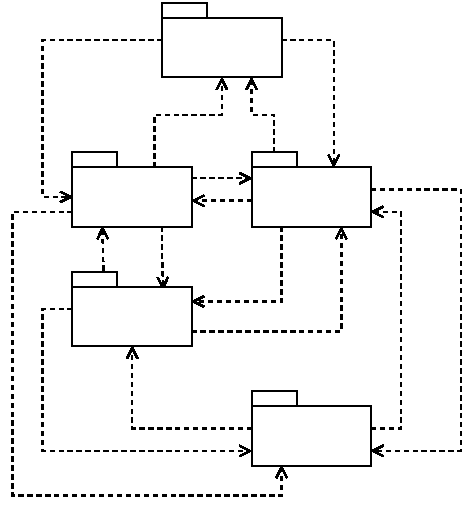
\includegraphics[width=.5\linewidth]{spaghetticode}
    \caption{Als code-onderdelen allemaal afhankelijk van elkaar zijn, 
    is het erg lastig om een onderdeel op zichzelf te wijzigen. 
    Dan spreekt men ook wel van spaghetticode.}
    \label{fig:spaghetticode}
    \index{spaghetticode}
\end{figure}

Natuurlijk kan de interne structuur 
van de software ook gevolgen hebben voor de gebruiker!
Denk bijvoorbeeld aan het tempo waarmee nieuwe features
kunnen worden uitgerold, de prestaties kunnen worden geoptimalizeerd 
of fouten kunnen worden opgespoord en hersteld. 
Het is makkelijker om de software te begrijpen, te veranderen 
of te verbeteren wanneer deze onderhoudbaar is ingericht. 
In projecten met een hoge structurele kwaliteit
zijn concepten duidelijk van elkaar gescheiden en zitten alleen die dingen
bij elkaar in een methode, klasse of package die bij elkaar horen.
Aan de andere kant wordt in dergelijke projecten flexibiliteit behouden
door de software samen te stellen uit verwisselbare onderdelen.
Vaak wordt daarbij gebruik gemaakt van bestaande oplossingen
zoals design patterns, libraries en frameworks, zodat de 
software meer gericht is op het oplossen van het 
daadwerkelijke probleem dan op de details van de uitvoerende technologie.

Het kan ook voorkomen dat een bepaalde nette structuur
minder efficiënt werkt of om een andere reden niet bij de oplossing past. 
In dat soort gevallen kan een ontwikkelaar ervoor kiezen, 
na de precieze impact te meten en de risico's af te wegen, om
op bepaalde plekken in de software voorrang te geven aan de prestaties tegenover 
de structuur. Het verdient aanbeveling om te beginnen met een nette structuur
en dan pas te optimaliseren, omdat binnen een geordende structuur het probleem
makkelijker op te sporen en te verbeteren is. Andersom
is het lastig om bijvoorbeeld performance-gerichte code meer onderhoudbaar te maken.

De beroemde computerwetenschapper 
Donald Knuth wees al decennia geleden op de gevaren van
voortijdige optimalisatie:
\blockquote{
The real problem is that programmers have spent
far too much time worrying about efficiency in the
wrong places and at the wrong times; premature
optimization is the root of all evil (or at least most of it)
in programming.
}{\cite{Knuth1974}, p. 671}

Ook wanneer maar één iemand aan de software werkt, 
is het van belang om aandacht te besteden aan de structuur. 
Het blijkt vaak erg lastig om code van een paar maanden geleden
nog goed te begrijpen! 
Veel developers vragen zich,
in totale verwarring, op enig punt in hun carrière af:
``Waar dacht ik in vredesnaam aan toen ik dit stuk code schreef?!''
Om nog maar te zwijgen over andermans code\ldots

Dit soort verbijstering zal minder plaatsvinden binnen
een georganiseerd project met duidelijke, betekenisvolle
abstracties, overzichtelijk georganiseerd en zonder verrassingen. 
Het is de kunst van een software developer om dit te bereiken!
Vakmannen en -vrouwen willen een doelbewust ontworpen oplossing, gerealiseerd met 
een geschikt gebruik van de programmeertaal volgens best practices, 
principles en patterns gecombineerd met nuttige comments, documentatie en tests.

We hebben nu in grote lijnen een idee gekregen van wat
structurele kwaliteit is. Hoe kunnen we de structuur van software beoordelen?
Hoe kunnen we onze software `netjes' inrichten? Het antwoord is te vinden
in de drie C's van structurele kwaliteit: 
separation of concerns, high cohesion en loose coupling.

\section{Separation of concerns}
\index{seperation of concerns}
Een onderhoudbaar systeem begint bij een systeem dat 
makkelijk te begrijpen is. Het zou mooi zijn als we 
terug kunnen vinden waar wat in ons systeem gebeurt!
Hoe doen we dat in het dagelijks leven?

Neem bijvoorbeeld de inrichting van een lade waar we bestek in doen.
Deze willen we optimaliseren voor het snel kunnen terugvinden
van het juiste bestek: vorken, messen en lepels in allerlei soorten en maten.
Om die reden hebben besteklades vaak een logische indeling, zodat 
het dekken van de tafel (of het opruimen na een afwas) minder tijd en moeite kost.
Het feit dat er een besteklade is waar we het bestek kunnen terugvinden
is natuurlijk ook al handig. Zo hoeven we niet door de hele keuken of eetkamer
te lopen om al het bestek bij elkaar te sprokkelen. 
Sterker nog: we hebben bepaalde voorwerpen (kookgerei, borden, bestek, etcetera) 
in de keuken en eetkamer gezet zodat we niet voor elke maaltijd het hele huis hoeven 
te doorzoeken! Er zijn natuurlijk uitzonderingen, maar we verdelen een huis 
in kamers op basis van de activiteiten die daarin plaatsvinden. 
Als we nog een stap uitzoomen, zie je dat een gemeente vaak ook een doelmatige
indeling heeft op basis van een bestemmingsplan. 
Industrie, woningen, winkelstraten: er zit een logische verdeling in!

Software kunnen we op eenzelfde manier benaderen.
Er zijn verschillende plekken in een softwaresysteem 
waar dingen gebeuren, maar we hoeven niet overal tegelijkertijd te zijn. 
We kunnen terugvinden waar wat precies gebeurt als we 
alle programmaonderdelen voorspelbaar indelen op basis van welke activiteiten
erin gebeuren. Het is dus niet erg om veel doelgerichte 
klassen en packages aan te maken,
mits de indeling en naamgeving bijdraagt 
aan de begrijpelijkheid en vindbaarheid.

Edsger Dijkstra, een van de (Nederlandse) grondleggers van 
softwareontwikkeling als zelfstandig studiegebied, zei het als volgt 
(onze cursivering):
\blockquote{
    Let me try to explain to you, what to my taste is characteristic for all intelligent thinking. 
    It is, that one is willing to study in depth an aspect of one's subject matter 
    \emph{in isolation} for the sake of its own consistency, 
    all the time knowing that one is occupying oneself only with \emph{one of the aspects}. 
    \newline\newline
    (...)
    \newline\newline
    It is what I sometimes have called "the separation of concerns", which, even if not perfectly possible, 
    is yet the only available technique for effective ordering of one's thoughts, 
    that I know of. This is what I mean by "focussing one's attention upon some aspect": 
    it does not mean ignoring the other aspects, it is just doing justice to the fact that 
    from this aspect's point of view, the other is irrelevant. 
    It is being one- and multiple-track minded simultaneously.
}{\cite{Dijkstra1982}, EWD447}

We willen ons systeem zó inrichten dat we verschillende aspecten
in verschillende onderdelen samenbrengen en we ons steeds maar met een
beperkt aantal onderdelen tegelijkertijd hoeven bezig te houden,
wanneer we de code schrijven, testen, verbeteren, 
uitbreiden, verwijderen en vervangen.

\subsection{Modules}
\index{module}
Een groepering van programmaonderdelen noemen we ook wel een \emph{module}.
In klasse-gebaseerde object-georiënteerde talen zoals Java en C\# 
zijn klassen en objecten de meest fundamentele modules. 
Hierin worden toestand en gedrag samengebracht in \emph{fields} en \emph{methods}:
de elementaire delen van een programmastructuur. 
Idealiter ziet een klasse moet op één aspect van functionaliteit 
en zijn de klasse en diens fields en methods voorzien van logische, menselijke namen.

\index{interface}
\emph{Interfaces} zijn andere fundamentele modules. 
Hiermee kan je bepaald gedrag van een subklasse afdwingen.
De publieke methoden van de implementerende klassen 
(diens \emph{application programming interface} of \emph{API}) moeten 
voldoen aan de in de interface opgenomen specificatie.
De methodenamen en parameter- en returntypes moeten overeenkomen met wat 
in de interface wordt afgedwongen.

\index{enumeration}
In veel programmeertalen heb je \emph{enumerations} (enums) 
om een beperkte set aan mogelijkheden aan te geven. Denk bijvoorbeeld aan 
de vier seizoenen van het jaar, de planeten van ons melkwegstelsel 
of de classificatiecodes van films. Met een beetje goede wil kan je 
een boolean zien als een enumeration van true en false.

Ten slotte heb je soms objecten nodig die geen gedrag nodig hebben
maar een groepering van een toestand vertegenwoordigen. 
In C\# kan je dit onderbrengen in een \emph{struct}. 
Sinds Java 16 kan je dit met \emph{records} bereiken.

\subsubsection{Packages}
\index{package}
In het \emph{filesystem} kan je bestanden groeperen door directories aan te maken.
Binnen een directory kan een bestandsnaam geen twee keer voorkomen, 
maar een bestandsnaam kan wel vaker voorkomen als de bestanden in verschillende
directories zitten. Met andere woorden: met directories kan je bestanden
bij elkaar brengen die bij elkaar horen, 
maar ook \emph{naming conflicts} (\emph{collisions}) voorkomen.

Dit is precies hoe Java's \emph{packages} en C\#'s \emph{namespaces} ook worden gebruikt:
om modules te groeperen en botsingen in naamgeving te voorkomen.
Net als directories kennen packages een \emph{recursieve} structuur.
Een package kan namelijk klassen, interfaces, enums en records bevatten, 
maar ook (sub)packages!

Packages zijn erg geschikt om aan te geven in welk algemene deelgebied (subdomein) 
van het softwaresysteem we ons begeven, maar ook om wat voor een soort logica het gaat
of om wat voor een specifieke deelfunctionaliteit het gaat.

\section{Structured design}
\index{structured design}
Het op een logische wijze inrichten van modules 
zorgt er over het algemeen voor dat een systeem makkelijker 
te navigeren is.
Dit zegt echter weinig over hoe je tot \emph{onderhoudbare} modules komt.

Dat was het centrale onderwerp 
van de \emph{structured design}-beweging 
in de jaren zeventig. Het doel was om 
de structurele kwaliteit van software te verbeteren.
Er waren veel problemen met het opdelen 
van software in losstaande onderdelen waar zelfstandig
door verschillende developers of teams aan gewerkt kon worden.
Hoewel het toen niet zozeer ging om object-georiënteerde code,
zijn de toen gevonden problemen, ideeën en oplossingen nog steeds relevant!
\blockquote{
(...) [W]e must be able to make a correction to piece A of the
system without introducing any unanticipated side effects in piece B 
- and, of course, that is precisely the problem that plagues 
many maintenance programmers!
\newline\newline
(...)
\newline\newline
Implementation, maintenance, and modification 
generally will be minimized when each piece of the system
corresponds to exactly one small, well-defined piece of the problem, 
and each relationship between a system's pieces corresponds only 
to a relationship between pieces of the problem.
}{\cite{YourdonConstantine1979}, pp. 17--18}

Bij het creëren van modules willen we erop letten dat 
we zaken groeperen die qua functionaliteit bij elkaar horen.  
Modules mogen alleen met elkaar interacteren voor zover dat 
nodig is voor de uitvoering van een bepaalde taak.
Op die manier verkleinen we de kans dat de wijziging in één onderdeel
automatisch gevolgen heeft voor de werking van een ander onderdeel.
Dit komt overeen met wat wordt verstaan onder \emph{modulariteit}, 
\index{modulariteit}
aldus \cite{ISO25010}: 
"[the] degree to which a system or computer program is composed of 
discrete components such that a change to one component has minimal impact
on other components".

De eigenschappen van modulariteit zijn uitvoerig onderzocht door
Yourdon en Constantine in hun werken over structured design.
Nog altijd analyseren software engineers hun werk aan de hand
van onder andere de termen \emph{cohesion} en \emph{coupling}.

\subsection{Cohesion}
\index{cohesion}
\index{samenhang}
Cohesion (of: \emph{samenhang}) ziet op de binnenkant van een module:
in hoeverre hangen de fields en methods binnen een klasse en de 
klassen binnen een package met elkaar samen?
We mogen immers verwachten dat alle interne elementen van een module 
met een duidelijk doel zijn ontworpen!
\blockquote{
Let us imagine (...) that there is some measure of 
functional (problem-defined) relatedness between pairs
of processing elements. In terms of this measure,
the most effectively modular system is the one for which
the sum of functional relatedness between pairs of elements
not in the same module is minimized; among other things, this
tends to minimize the required amount of intermodular connections
and the amount of intermodular coupling.
\newline\newline
(...)
\newline\newline
What we are considering is the \emph{cohesion} of each module
in isolation -- how tightly bound or related its internal elements
are to one another.
}{\cite{YourdonConstantine1979}, p. 95}

Wanneer een klasse heel veel methoden bevat die elk op een ander stuk
functionaliteit zien of een package allerlei klassen bevat die vrij weinig
met elkaar te maken hebben, spreken we van \emph{low cohesion}. Dit is vaak
een teken om de code te herstructureren. Zie Figuur~\ref{fig:cohesion}.
Meestal willen we dan een klasse opsplitsen
of klassen op een meer samenhangende manier verdelen binnen packages.
We willen ons richten op \emph{high cohesion}: de verantwoordelijkheden van een
klasse of package zien op gelijksoortige onderwerpen of functionaliteiten.
Zo wil je alles dat met security te maken heeft, 
waaronder registreren, inloggen, authentication en authorization,
in een andere module stoppen dan alles dat met het 
opnemen of storten van chips te maken heeft.

\begin{figure}[H]
    \centering
    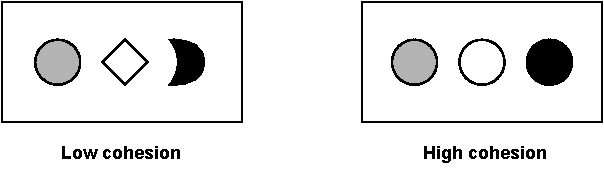
\includegraphics[width=.7\linewidth]{cohesion}
    \caption{Low cohesion versus high cohesion.
    Een samenhangende module brengt verschillende gerelateerde zaken samen 
    en ziet niet op teveel aspecten tegelijkertijd.}
    \label{fig:cohesion}
\end{figure}

Stel je een systeem voor waarin regelmatig een bestand moet worden uitgelezen
en opgeslagen worden van het bestandssysteem. In plaats van dat je op elke plek 
opnieuw op de details van het bestandssysteem in gaat, zou je een toegewijd systeemonderdeel kunnen 
ontwerpen dat enkel verantwoordelijk is voor het lezen en schrijven van bepaalde data.
Op die manier is er één duidelijk punt waarin bestanden worden uitgelezen en weggeschreven.

\subsection{Coupling}
\index{coupling}
\index{koppeling}
Coupling (\emph{koppeling}) ziet op de relaties tussen modules.
In hoeverre is een bepaalde module \emph{afhankelijk} van een andere module?
\blockquote{
The measure that we are seeking is known as \emph{coupling};
it is a measure of the \emph{strength} of interconnection. 
Thus, ``highly coupled'' modules are joined by strong 
interconnections; ``loosely coupled'' modules are joined by
weak interconnections; ``uncoupled'' or ``decoupled'' modules 
have \emph{no} interconnections and are, thus, \emph{independent}
(...). 
\newline\newline
Obviously, what we are striving for is loosely coupled systems
-- that is, systems in which one can study (or debug, or maintain)
any one module without having to know very much about any other
modules in the system.
}{\cite{YourdonConstantine1979}, p. 76}

We willen werken in losgekoppelde systemen. In dat soort systemen
hebben wijzigingen in de ene module slechts een beperkte impact 
op een andere module. Dat komt omdat er spaarzaam wordt omgegaan 
met de afhankelijkheden tussen modules. Er is dan sprake van
\emph{loose coupling}. In de meeste gevallen willen we 
\emph{tight coupling} vermijden. Zie Figuur~\ref{fig:coupling}.

\begin{figure}[H]
    \centering
    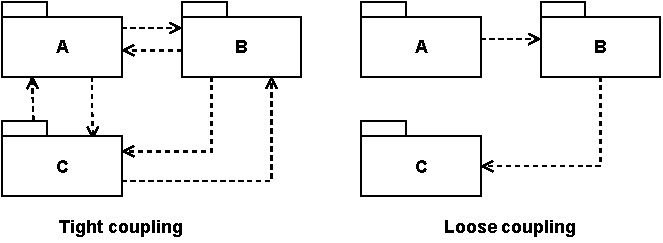
\includegraphics[width=.7\linewidth]{coupling}
    \caption{Tight coupling versus loose coupling.
    In een losgekoppeld systeem wordt er doelbewust omgegaan 
    met afhankelijkheden.}
    \label{fig:coupling}
\end{figure}

\index{afhankelijkheid}
\index{dependency} 
Een andere manier om over coupling na te denken is door te kijken naar hoeveel 
de ene module weet van een andere module. Hierin kan je verschillende gradaties
herkennen: kent de ene module de andere niet, kent deze slechts een publieke methode 
of is deze bekend met alle details die zich binnen de andere module afspelen?
Dat maakt nogal een verschil!

Zie nogmaals het voorbeeld van het bestandssysteem. In plaats van dat we op 
verschillende plekken bezig moeten zijn met de details van opslag, hebben we 
een module gemaakt die verantwoordelijk is voor het uitlezen en wegschrijven 
van bestanden. Gebruikers van die klasse hoeven alleen maar bekend te zijn met de 
diesnten die door die module worden geboden en niet met alle details van bestandsafhandeling.
Op die manier wordt de coupling beperkt.

Een klasse kan op een aantal manieren gekoppeld zijn aan een andere
klasse. Zo kan een object van een bepaalde klasse bijvoorbeeld de publieke methoden
aanroepen van een andere klasse, kan een object zijn opgebouwd uit andere
klassen (\emph{associatie}) of kan er sprake zijn van
overerving (\emph{generalization}) of implementatie (\emph{realisatie}).

Hoewel cohesion (de samenhang binnen een module) 
en coupling (de relatie tussen modules) 
twee verschillende begrippen zijn, is er in de praktijk 
een verband te bespeuren tussen de twee.
\blockquote{
Clearly, cohesion and coupling are interrelated. The greater
the cohesion of individual modules in the system, the lower
the coupling between modules will be. In actual practice,
these two measures are correlated; that is, on the average,
as one increases, the other decreases; but the correlation is 
not perfect.
}{\cite{YourdonConstantine1979}, p. 96}

Over het algemeen kunnen we dus zeggen dat de mate van koppeling
tussen modules kleiner is wanneer modules meer interne samenhang vertonen.
Modules hoeven dan immers minder informatie met elkaar te delen.

\section{Samenvatting}
In dit hoofdstuk hebben we onderzocht wat we kunnen verstaan onder
structurele kwaliteit en hoe we dit over het algemeen kunnen bereiken.

\begin{defbox}{Structurele kwaliteit}
    Structurele kwaliteit ziet vooral op de onderhoudbaarheid
    van een softwareproject.
    \newline\newline
    Een softwareproject heeft in algemene zin 
    een goede structuur als deze is opgedeeld in kleine,
    opzichzelf staande modules die intern veel samenhang 
    en met elkaar beperkt koppeling vertonen.
    \newline\newline
    Met andere woorden, we willen modulariteit dankzij:
    \begin{enumerate}
        \item Separation of concerns
        \item High cohesion
        \item Loose coupling
    \end{enumerate}
\end{defbox}



\chapter{Object-georiënteerd programmeren in Java}
In voorgaande cursussen is er al meer aandacht besteed aan 
object-georiënteerd programmeren in Java, maar het kan nooit kwaad 
om hier nogmaals het een en ander te herhalen. 

We gaan eerst kort in op Java en de Java Virtual Machine (JVM) om
vervolgens nader in te gaan op allerlei aspecten die je tegenkomt 
wanneer je in Java programmeert.

\section{Java}
Java is een veelgebruikte programmeertaal
waarmee allerlei verschillende soorten applicaties kunnen
worden gemaakt. De taal is in 1995 uitgebracht en is oorspronkelijk
ontworpen door James Gosling bij Sun Microsystems (later overgenomen door
Oracle). 

De kracht van Java zit hem in de JVM, 
een manier om Java (en andere programmeertalen die JVM-compatible zijn) 
te kunnen uitvoeren op verschillende soorten apparaten.

\section{De Java Virtual Machine (JVM)}
De CPU (\textit{Central Processing Unit} of \textit{processor}) 
in onze computer kan alleen machinecode lezen 
die hoort bij de betreffende CPU-architectuur.
Omdat machinecode lastig is te lezen, schrijven en organiseren
voor mensen, zijn er hogere programmeertalen 
uitgevonden (\textit{high-level languages}). 
Dit zijn talen die in meer of mindere mate verder verwijderd zijn van 
de concrete hardware en dus op een hoger abstractie niveau werken.
Er zijn talen die relatief dicht op de hardware zitten (zoals C en C++)
en er zijn talen waarbij de gebruiker vrijwel geen besef hoeft te hebben 
van de onderliggende hardware (zoals Python en JavaScript).
Talen als Java en C# zitten er een beetje tussenin.

\subsection{Compilatie}
Er zijn programmeertalen die eerst door de gebruiker moeten worden 
omgezet om te kunnen uitgevoerd. Dit noemen we \textit{compilatie}.
Een \textit{compiler} leest broncode van de ene taal en zet het om naar code
in de andere taal. Vaak gaat het hier om omzetting van een hogere taal 
(zoals C of C++) naar een lagere taal (zoals een assembly-taal of machinecode).
Zie Figuur~\ref{fig:compiler}.
Compilers zijn vaak erg knap geprogrammeerd. Niet alleen ondersteunen ze 
veel CPU-architecturen als uitvoer, vaak worden er tijdens compilatie 
allerlei optimalisaties aangebracht om de code sneller te laten draaien.
Hierdoor duurt het compileren mogelijk wat langer, maar de eindgebruiker
heeft er later profijt van!

\begin{figure}[H]
    \centering
    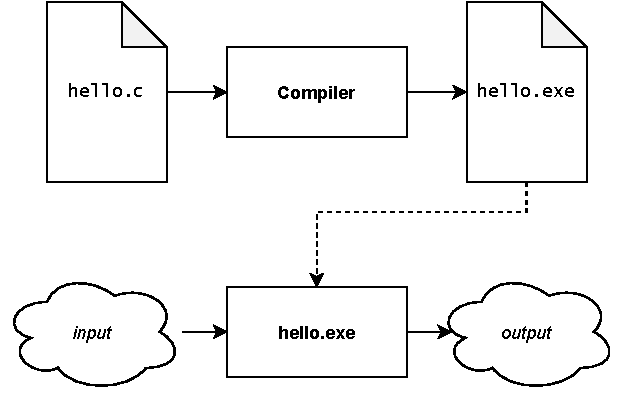
\includegraphics[width=.7\linewidth]{compilation}
    \caption{Compilatie, versimpeld weergegeven.}
    \label{fig:compiler}
    \index{compiler}
\end{figure}

Vaak moet de programmeur op de een of andere manier aan de compiler duidelijk 
maken welke bestanden allemaal samen moeten worden gevoegd in het uitvoerbestand.
Het kan soms een hele klus zijn om compilers met de hand in te stellen, 
hiervoor kunnen \textit{build tools} en 
\textit{integrated development environments (IDEs)}
uitkomst bieden. Dit soort tools zorgen ervoor dat programmeurs 
makkerlijker met de broncode kunnen werken.

\subsection{Interpretatie}
Een andere aanpak om hogere talen om te zetten naar machinetaal is door 
gebruik te maken van een \textit{interpreter}. Dit is een programma dat 
de hogere taal inleest en het rechtstreeks omzet naar uitvoering op de 
CPU. Zie Figuur~\ref{fig:interpreter}. Dit heeft als voordeel dat er geen compilatiestap meer nodig is, 
maar als nadeel dat er minder tussentijdse optimalisaties uitgevoerd worden.

\begin{figure}[H]
    \centering
    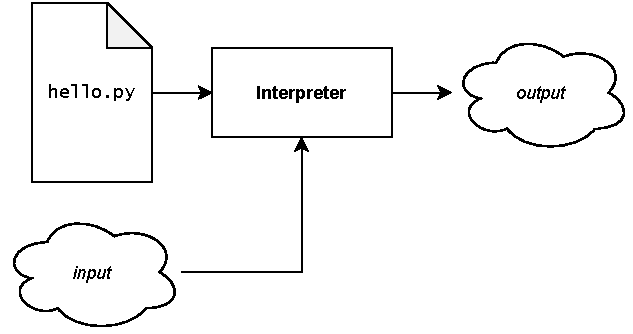
\includegraphics[width=.7\linewidth]{interpretation}
    \caption{Interpretatie, versimpeld weergegeven.}
    \label{fig:interpreter}
    \index{interpreter}
\end{figure}

Python en JavaScript zijn voorbeelden van geïnterpreteerde talen. Web browsers
hebben een ingebouwde JavaScript-interpreter om gebruikersinteractie te verwezelijken.

\subsection{Tussentalen}
Hogere programmeertalen zijn wat syntax en grammatica betreft vaak 
erg complex. Daarnaast compilers en interpreters veel CPU-architecturen 
ondersteunen met elk een eigen soort machinecode als uitvoerformaat.
Om deze complexiteit op te splitsen in beheersbare onderdelen, 
werken sommige talen met een soort "algemene" tussentaal. Deze algemene,
simpelere tussentaal wordt dan uitgelezen door een soort interpreter 
die dit weet uit te voeren voor verschillende CPU-architecturen.
Dit soort talen werken dus met een combinatie van een compiler en 
een interpreter, zie Figuur~\ref{fig:tussentaal}.

\begin{figure}[H]
    \centering
    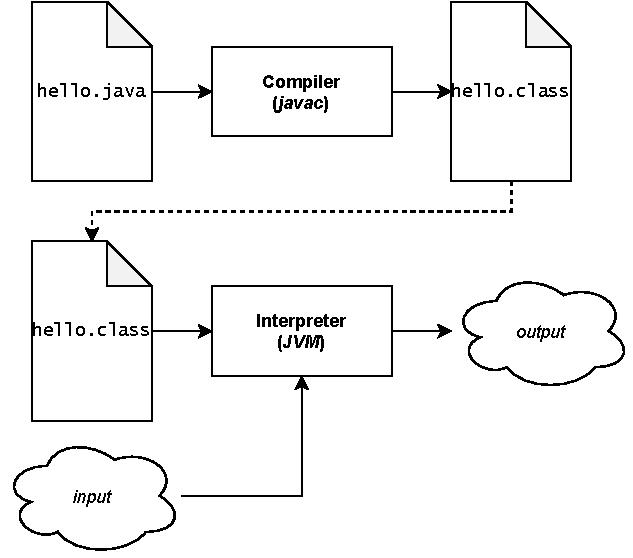
\includegraphics[width=.7\linewidth]{tussentaal}
    \caption{Tussentaal, versimpeld weergegeven.}
    \label{fig:tussentaal}
    \index{tussentaal}
\end{figure}

Java is een voorbeeld van een taal waarvan 
de broncode (\textit{Java-code}) eerst wordt 
omgezet in een tussentaal (\textit{bytecode}),
welke vervolgens wordt uitgevoerd door de \textit{Java Virtual Machine (JVM)}.
Nieuwere talen zoals \textit{Kotlin}, \textit{Clojure} en \textit{Scala} 
compileren ook naar bytecode en zijn dus ook uitvoerbaar door de JVM!

Een ander voorbeeld van een taal die met een tussentaal werkt is C\#.
Daarin wordt C\#-code eerst omgezet naar een 
\textit{intermediate representation (IR)} om vervolgens te worden uitgevoerd
door de \textit{Common Language Runtime (CLR)}.

\section{Typesysteem}
Voor een CPU is alle data binair: het bestaat uit enen en nullen.
In werkelijkheid zit er betekenis achter deze bits. 
De ene keer gaat het om een heel getal, de andere keer om een kommagetal
en weer een andere keer om een tekst of een lijst van getallen.

In een hogere programmeertaal maken we dit onderscheid middels \textit{data types}.
Het data type bepaalt wat je allemaal met een stuk data kunt doen en in hoeverre het 
compatibel is met een ander data type.

\subsection{Sterk en statisch getypeerd}
Er zijn programmeertalen die heel vergevingsgezind zijn ten aanzien van de types
die de programmeur gebruikt. Sommige talen, zoals Python, converteren waar mogelijk 
stilzwijgend data van het ene type naar dat van een ander type. Dat zie je veel 
in \textit{zwak getypeerde} talen.
Java is niet zo'n taal, maar is \textit{sterk getypeerd}. 
Dit houdt in dat de programmeur zijn datatypes nadrukkelijk moet aangeven
en de compiler klopt of de juiste types worden gebruikt. Hoewel dit erg 
wennen is als je nog wat minder bekend bent met de verschillende types,
voorkomt dit een aantal programmeerfouten en kan de compiler gemakkelijker
bepaalde optimalisaties uitvoeren.

In Java wordt \textit{type checking} in de compiler uitgevoerd. Er wordt 
puur op basis van de broncode gekeken of de gedeclareerde types en de beschreven 
operaties kloppen. Wanneer de types voor de compiler moeten worden aangegeven in 
een programmeertaal, noem je deze taal \textit{statisch getypeerd}. Talen waarin 
je het typesysteem vooral tijdens runtime tegenkomt (dus na compileren, bij uitvoering) 
zijn \textit{dynamisch getypeerde} talen als JavaScript en Python.

\subsection{Value types versus reference types}
In Java kennen we \textit{value types} en \textit{reference types}.
Value types zijn types die in het geheugen worden opgeslagen (in de \textit{stack}) 
op basis van hun waarde. 
Zo staat de integer 42 altijd op dezelfde plek in het geheugen voor een bepaalde 
methode-aanroep, onafhankelijk van welke variabele ernaar wijst. 

Reference types worden in het geheugen opgeslagen (in de \textit{heap}) 
op basis van hun instantie, hun identiteit.
Twee objecten worden op verschillende geheugenadressen opgeslagen, zelfs als hun 
waarden hetzelfde zijn!

Anders dan in bijvoorbeeld C++ wordt er in Java geen onderscheid gemaakt naar 
\textit{pass-by-value} of \textit{pass-by-reference}. We hoeven dus geen rekening 
te houden met pointer-logica. Alle method calls in Java werken 
volgens het principe van \textit{pass-by-value}, ook wanneer er een reference
type wordt meegegeven. De reference wordt dan als waarde meegegeven middels een
parameter. Je kan de reference zelf niet aanpassen, slechts de waarden waarnaar 
wordt gerefereerd. Je kan bijvoorbeeld een referentie naar een object meegeven 
als een parameter van een methode. 
Dat object kan je aanpassen via die referentie -- mits de publieke methodes dat toelaten binnen 
de methode. Je kan er niet voor zorgen dat er ineens een ander object op dezelfde plek in 
het geheugen komt. Dit kan in sommige andere talen wel, 
waar het voor enige verwarring kan zorgen onder developers.

\subsection{Primitive types}
\textit{Primitive types} zijn basale standaardtypen die door Java worden geboden.
Er zijn 8 verschillende primitive types in Java.
Zie Tabel~\ref{table:primitive-types}. 

\begin{table}[H]
    \centering
    \begin{tabularx}{\textwidth}{
        |>{\raggedright}l|>{\raggedright}X|>{\raggedright\arraybackslash}X|
    }
    \hline
    \textbf{Type} & \textbf{Betekenis} & \textbf{Voorbeeld} \\ \hline
        \textit{boolean}
        & een binaire waarheidswaarde van \texttt{true} of \texttt{false}
        & \texttt{boolean isGood = true;} \\ \hline
        \textit{byte}
        & een geheel getal met een grootte van 8 bits \newline 
        (van \(-128\, (-2^7)\) t/m \(127\, (2^7 - 1)\))
        & \texttt{// Base 10: 5} \newline \texttt{byte bits = 0b101;} \\ \hline
        \textit{short}
        & een geheel getal met een grootte van 16 bits \newline
        (van \(-32.768\, (-2^{15})\) t/m \(32.767\, (2^{15} - 1)\))
        & \texttt{short smallNumber = 1021;} \\ \hline
        \textit{integer}
        & een geheel getal met een grootte van 32 bits \newline
        (van \(-2.147.483.648\, (-2^{31})\) t/m \(2.147.483.647\, (2^{31} - 1)\))
        & \texttt{int largeNumber = 2312121;} \\ \hline
        \textit{long}
        & een geheel getal met een grootte van 64 bits \newline
        (van \(-2^{63}\) t/m \(2^{63} - 1\))
        & \texttt{long largerNumber = 323121211L;} \\ \hline
        \textit{float}
        & een komma-getal met een grootte van 32 bits \newline
        (van \(-2^{31}\) t/m \(2^{31} - 1\))
        & \texttt{float pi = 3.14F;} \\ \hline
        \textit{double}
        & een komma-getal met een grootte van 64 bits \newline
        (van \(-2^{31}\) t/m \(2^{31} - 1\))
        & \texttt{double pi = 3.1415D;} \\ \hline
        \textit{char}
        & een tekstteken met een grootte van 16 bits
        & \texttt{char letterX = `X`;} \\ \hline
    \end{tabularx}
    \caption{Java's primitive types}
    \label{table:primitive-types}
    \centering
\end{table}

Primitive types zijn value types, ze zijn dus ook immutable. Je kan ze wel 
overschrijven, maar niet (gedeeltelijk) aanpassen. 
In Java kunnen primitive types aangegeven worden met een kleine letter of een 
grote letter. Met een kleine letter (bijvoorbeeld \texttt{int}) 
verwijs je naar een \textit{unboxed type}. 
Dit zijn rauwe types zonder methodes; het zijn geen objecten.
Begint het type met een hoofdletter (bijvoorbeeld \texttt{Integer}), d
an is het een \textit{boxed type} en 
gedraagt het zich wel als een object. De JVM zorgt op veel plekken voor 
autoboxing. Dat betekent dat het op veel plekken niet zoveel uitmaakt of je 
verwijst naar de boxed of de unboxed variant. 

Wil je een methode aanroepen op 
een object, maar gaat het om de unboxed variant? Dan kan je het eerst omzetten 
door de waarde aan de constructor mee te geven. In de praktijk is het handig om 
zoveel mogelijk boxed types te gebruiken.

\subsection{Strings}
Strings zijn bedoeld om reeksen van teksttekens aan te geven.
Een string is geen primitive type in Java. Je kan er dus alleen 
naar verwijzen via \texttt{String}, een object van het type String. 
Omdat ze zoveel voorkomend zijn hebben ze een bijzonder karakter in Java. 
Zo kan je met een \textit{string literal} een String aanmaken:
\texttt{String text = "Hello world!"}. 

Net als primitive types zijn Strings ontworpen met het idee van 
immutability. Dat wil zeggen dat, hoewel het reference types zijn, hun waarde 
niet deels kunnen worden aangepast. Deze kan slechts in zijn geheel worden 
overschreven.

\section{Objecten en klassen}
Java is ontworpen met het idee van object-oriëntatie:
objecten zijn de centrale abstracties waarmee we ons werk doen.
Dit leidt tot een aantal voordelen, maar vereist ook wat denkwerk
bij het ontwerpen en realiseren van objecten. Hierover in een ander hoofdstuk meer.

We duiken in een aantal van Java's belangrijkste object-georiënteerde mogelijkheden
aan de hand van het domein van tweedimensionale geometrische vormen, zie Figuur~\ref{fig:shapes}.
\begin{figure}[H]
    \centering
    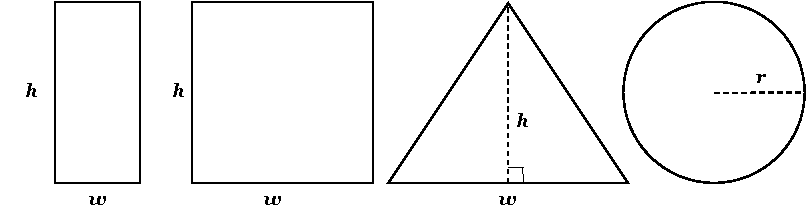
\includegraphics[width=.7\linewidth]{shapes}
    \caption{Geometrische vormen en hun dimensies.}
    \label{fig:shapes}
\end{figure}

Java is een \emph{klasse-gebaseerde} object-georiënteerde programmeertaal.
Dit betekent dat de programmeur nieuwe objecten kan definiëren door hiervoor 
nieuwe klassen aan te maken. Een klasse (\textit{class}) is een soort 
blauwdruk van een object en bepaalt het type van het object.
Zie bijvoorbeeld de \texttt{Rectangle}-klasse die ten grondslag kan 
liggen aan verschillende rechthoek-instanties met verschillende configuraties.
Zie Voorbeeld~\ref{code:rectangle}.

\begin{listing}[H]
\begin{minted}[linenos]{java}
public class Rectangle implements Shape2D {
    private Integer height;
    private Integer width;

    public Rectangle(Integer height, Integer width) {
        this.height = height;
        this.width = width;
    }

    public Double calculateArea() {
        return (double) (this.height * this.width);
    }

    public Boolean isLargerThan(Shape2D other) {
        return this.calculateArea() > other.calculateArea();
    }
}
\end{minted}
\caption{Een klasse voor een rechthoek.}
\label{code:rectangle}
\end{listing}

In \ref{code:rectangle} zien we dat \texttt{Rectangle} een klasse is
die een interface implementeert met de naam \texttt{Shape2D} 
(een tweedimensionale geometrische vorm). De klasse heeft 
dus het type \texttt{Rectangle} en als supertype \texttt{Shape2D}. Dit betekent 
dat we een object-instantie van het type \texttt{Rectangle} kunnen invullen 
waar om een \texttt{Shape2D} wordt gevraagd. Dat is een voorbeeld van polymorfisme.
Over interfaces en polymorfisme later meer, maar het is van belang om in te zien dat 
we verschillende implementaties kunnen maken van \texttt{Shape2D}. Zie Figuur~\ref{fig:uml-shapes}.

\begin{figure}[H]
    \centering
    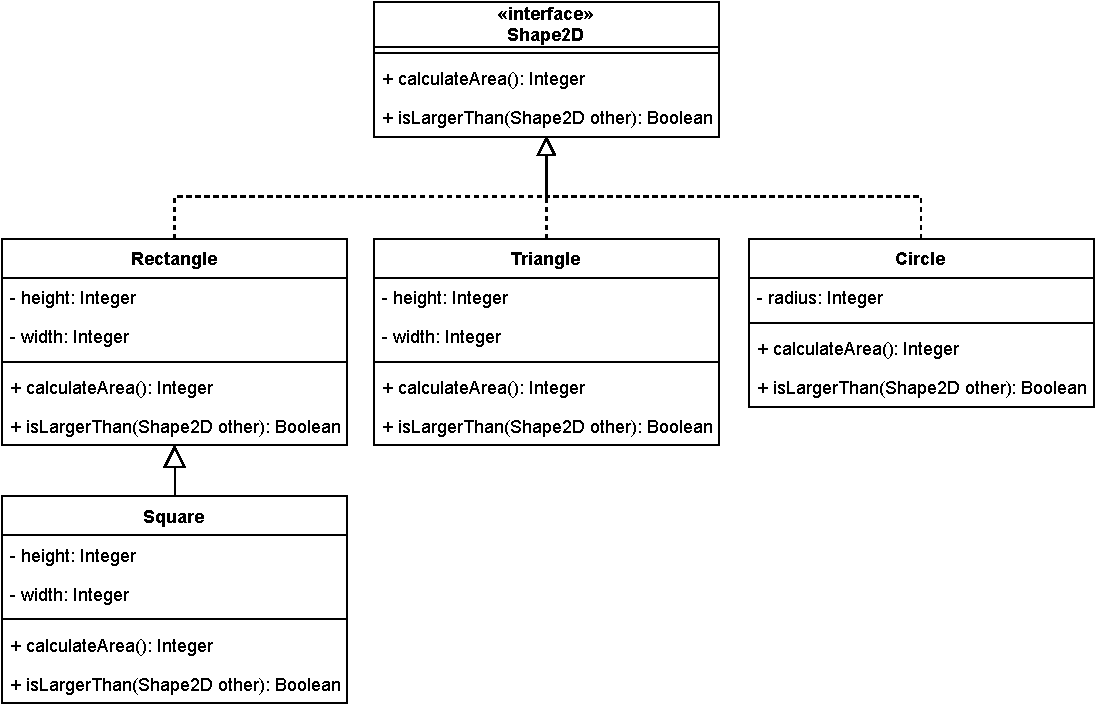
\includegraphics[width=.9\linewidth]{uml-shapes}
    \caption{Een UML klassendiagram van de verschillende shapes, inclusief realisatie en overerving.}
    \label{fig:uml-shapes}
\end{figure}

Objecten brengen toestand (\textit{fields}) en gedrag (\textit{methods}) onder 
in één eenheid, waarmee we kunnen praten via publieke methodes. 
Op die manier verbergt het object de interne complexiteit en wordt het onmogelijk
om van buiten het object afhankelijk te worden van hoe het object intern te werk gaat:
de implementatiedetails zijn verborgen.

\subsection{Fields}
De toestand van een object wordt bijgehouden in \textit{fields}
(velden, soms ook: \textit{attributes} of \textit{properties}).
In Voorbeeld~\ref{code:rectangle} kan je zien dat de fields zijn opgenomen in regels
2 en 3, namelijk de width (breedte) en height (hoogte), beide van het type Integer.

Het declareren van fields doen we vaak bovenin de klasse. Meestal beschrijf je een 
aantal modifiers (zie hierna), het type van de field en vervolgens 
de naam van het field. Het is belangrijk om een leesbare, menselijke naam te gebruiken 
die past bij het domein van ons systeem. 

We kunnen binnen een objectinstantie toegang krijgen tot 
een field door ernaar te verwijzen via \texttt{this}, bijvoorbeeld: \texttt{this.width}.

\subsection{Methods}
Met \textit{methods} (methodes) kunnen we gedrag toekennen aan een object.
We declareren een methode door deze in een klasse op te nemen. Een dergelijke 
declaratie (een \textit{method signature}) heeft de volgende onderdelen:
\begin{enumerate}
    \item \textit{modifiers}: geven bijzonderheden van de methode aan, 
    zoals bijvoorbeeld de zichtbaarheid vanuit andere klassen (zie hierna)
    \item \textit{return-type}: geeft aan wat voor een type er terug wordt gegeven 
    na het aanroepen van de methode
    \item \textit{parameter-types en -namen}: als er parameters zijn, 
    geef je deze aan met een type en een naam (zie: Voorbeeld~\ref{code:rectangle}, regels 14-16)
    \item \textit{checked exceptions die gegooid kunnen worden}: 
    als er checked exceptions (fouten die afgehandeld moeten worden) gegooid kunnen worden
    die niet in de methode worden afgehandeld, dien je deze te specificeren door \texttt{throws} 
    met daarachter de te gooien exception types
\end{enumerate}

Een voorbeeld is te vinden in Voorbeeld~\ref{code:rectangle}, regels 10-12 en regels 14-16.
Op deze manier hebben we de mogelijkheid toegevoegd om van een bestaande rechthoek
de oppervlakte te berekenen en de grootte te vergelijken met een ander tweedimensionale vorm.

Merk trouwens op dat we de oppervlakte omzetten van een integer naar een double. Dat doen we met de 
\textit{type cast} \texttt{(double)}. Java past hier autoboxing toe door de uiteindelijke
\texttt{double} automatisch om te zetten naar de in de return type aangegeven \texttt{Double}.

Methodes zijn, zoals je ziet, een krachtige manier om betekenis toe te voegen aan een project:
door de namen en typen van klassen en velden te lezen zien we met welke data we te maken hebben,
door de namen, return-typen en parameter-typen van methodes te lezen zien we wat we allemaal 
met een object kunnen doen.

Vaak kunnen we methods onderscheiden in \textit{queries}, die een waarde teruggeven
zonder iets aan te passen of een (externe) actie uit te voeren, en 
\textit{commands}, die iets aanpassen of iets anders doen en niet per se een 
waarde hoeven terug te geven. Het type \texttt{void} is gelijkwaardig aan \texttt{null}
(de afwezigheid van een waarde), maar geeft aan dat er geen intentie is dat de methode 
iets teruggeeft. Een query kan per definitie geen void als return type hebben. Er kan wel 
\texttt{null} terugkomen, wat aangeeft dat er geen waarde `gevonden' kon worden. 
In plaats van null is het overigens het overwegen waard om Optional te gebruiken.

We roepen een methode aan op een objectinstantie door tussen de instantie en de methode 
een punt te zetten en er haakjes achter te zetten. Moeten we argumenten meegeven voor 
de parameters, dan vullen we deze in de haakjes in. Zie Voorbeeld~\ref{code:method-call},
regel 4.

\begin{listing}[H]
\begin{minted}[linenos]{java}
Shape2D rectangleA = new Rectangle(10, 20);
Shape2D rectangleB = new Rectangle(20, 30);

if (rectangleB.isLargerThan(rectangleA)) {
    System.out.println("B is larger than A");
}

\end{minted}
\caption{We maken twee rechthoeken aan en kijken 
of rechthoek B groter is dan rechthoek A.}
\label{code:method-call}
\end{listing}

\subsubsection{Constructor}
In Voorbeeld~\ref{code:rectangle}, regels 5-7, zien we de constructor
van onze rechthoek. Het is een bijzonder soort methode die een objectinstantie
van een klasse maakt. We zien in Voorbeeld~\ref{code:method-call}, regels 1 en 2,
hoe we zo'n constructor in een andere klasse kunnen aanroepen. We kennen de instantie 
toe aan een variabele. Deze wijst nu naar een plekje in het geheugen waar de 
\texttt{Rectangle}-instantie is opgeslagen tijdens de duur van de applicatie.

Merk op dat we bij het declareren van de variabele het supertype hebben aangegeven.
Op deze manier zouden we ook de constructor van een andere klasse kunnen aanroepen 
en aan de variabele toekennen, mits deze ook \texttt{Shape2D} implementeert.

Onze IDE kan op basis van de aanwezige fields gemakkelijk een constructor genereren.
In IntelliJ kan je hiervoor op Windows en Linux de hotkeys \texttt{Alt + Insert} gebruiken, 
op MacOS \texttt{Command + N}.

\subsubsection{Getters en setters}
Op dit moment zijn de enige waardes die we uit ons object kunnen krijgen 
de oppervlakte (omgezet naar een double) en of het object groter is dan een ander object (Boolean).
De hoogte en breedte van een rechthoek kunnen we niet uit de objectinstantie opvragen.

Hoewel we hiermee voorzichtig moeten zijn omdat we zo koppeling op de 
implementatiedetails van het object mogelijk maken, kunnen we getters 
(of: \textit{accessors}) toevoegen 
om bij verborgen (\textit{private}) fields te kunnen.

Ook kunnen we de Rectangle van buitenaf niet aanpassen, als we eenmaal een instantie.
Een beetje zoals een \textit{value type}, moeten we een nieuwe Rectangle maken 
als we deze willen 'aanpassen'. Dit maakt code over het algemeen een stuk makkelijker 
te begrijpen (en en te parallelliseren). Vinden we dit wat minder belangrijk
(en vinden we koppeling op de interne toestand toelaatbaar), dan kunnen we 
ervoor kiezen om setters (ook: \textit{mutators}) toe te voegen. 
Zie Voorbeeld~\ref{code:accessors}.

\begin{listing}[ht]
\begin{minted}[linenos]{java}
public class Rectangle implements Shape2D {
    private Integer height;
    private Integer width;

    public Rectangle(Integer height, Integer width) {
        this.height = height;
        this.width = width;
    }

    // Other methods...

    public Integer getHeight() {
        return this.height;
    }

    public Integer getWidth() {
        return this.width;
    }

    public void setHeight(Integer height) {
        this.height = height;
    }

    public void setWidth(Integer width) {
        this.width = width;
    }
}
\end{minted}
\caption{Met getters kunnen we toegang krijgen tot fields en met setters kunnen we ze wijzigen.
Omdat de interne toestand niet meer is afgeschermd, 
brengt dit wel risico's mee ten aanzien van koppeling.}
\label{code:getters-setters}
\end{listing}

Ook dit is eenvoudig te genereren door je IDE op basis van de aanwezige fields.
In IntelliJ kan je hiervoor op Windows en Linux de hotkeys \texttt{Alt + Insert} gebruiken, 
op MacOS \texttt{Command + N}.

\subsubsection{Gelijkwaardigheid: \texttt{equals()} en \texttt{hashCode()}}
Omdat objecten reference types zijn, wordt de \texttt{equals}-methode standaard gebaseerd 
op het geheugenadres van de instanties. Alleen als deze gelijk zijn is sprake van 
hetzelfde object, zie Voorbeeld~\ref{code:identity-equality}.

\begin{listing}[H]
\begin{minted}[linenos]{java}
Shape2D rectangleC = new Rectangle(20, 30);
Shape2D rectangleD = new Rectangle(20, 30);

// Prints: false
System.out.println(rectangleC.equals(rectangleD));

Set<Shape2D> shapes = new HashSet<>();
shapes.add(rectangleC);

// Prints: false
System.out.println(shapes.has(rectangleD));

\end{minted}
\caption{Standaard \texttt{equals}- en \texttt{hashCode}-methodes: 
gelijkwaardigheid op basis van identiteit.}
\label{code:identity-equality}
\end{listing}

Dit is niet altijd wat we willen. Soms willen we gelijkwaardigheid
vaststellen op basis van waardes, in plaats van identiteit. Daarvoor kunnen we 
de \texttt{equals}-methode overschrijven.

De \texttt{hashCode}-methode is vergelijkbaar, maar ziet op hoe objecten 
efficient kunnen worden bewaard in 
een \texttt{HashMap}, \texttt{HashSet} of \texttt{HashTable}.
Normaliter wordt dat ook op basis van geheugenadres gedaan. Ook dat is te overschrijven.

\begin{listing}[H]
\begin{minted}[linenos]{java}
public class Rectangle implements Shape2D {
    private Integer height;
    private Integer width;

    // Constructor + other methods...

    @Override
    public boolean equals(Object o) {
        if (this == o) return true;
        if (o == null || getClass() != o.getClass()) return false;
        Rectangle rectangle = (Rectangle) o;
        return Objects.equals(height, rectangle.height) 
            && Objects.equals(width, rectangle.width);
    }

    @Override
    public int hashCode() {
        return Objects.hash(height, width);
    }
}
\end{minted}
\caption{Door IDE gegenereerde \texttt{equals}- en \texttt{hashCode}-methodes.}
\label{code:hashcode-equals}
\end{listing}

Beide methodes zijn te genereren door onze IDE, zie Voorbeeld~\ref{code:hashcode-equals}
Je zult zien dat onze IDE zelfs een aantal randgevallen afdekt in de \texttt{equals}-methode!
In IntelliJ kan je hiervoor op Windows en Linux wederom 
de hotkeys \texttt{Alt + Insert} gebruiken, op MacOS \texttt{Command + N}.
Na deze toevoegingen printen beide gevallen uit Voorbeeld~\ref{code:identity-equality}
\texttt{true}!

\subsection{Inheritance}
Inheritance (\textit{overerving}) is een veelgebruikt maar controversieel mechanisme in Java 
om aan te geven dat een subklasse (ook: \textit{child}) is afgeleid van 
een superklasse (ook: \textit{parent}) en dat deze subklasse  
fields en methods overneemt van deze superklasse.

Dit is te zien in Voorbeeld~\ref{code:inheritance}. Een vierkant is een 
specifiek soort rechthoek, namelijk een rechthoek met gelijke zijden.
Daarom roepen we in de constructor van Square de constructor aan van 
de superklasse, Rectangle, middels de \texttt{super}-methode en we vullen 
de size voor zowel de height als de width in.

\begin{listing}[H]
\begin{minted}[linenos]{java}
public class Square extends Rectangle {
    public Square(Integer size) {
        super(size, size);
    }
}
\end{minted}
\caption{Een Square is een specifiek soort Rectangle.}
\label{code:inheritance}
\end{listing}

Wanneer we een Square-instantie hebben kunnen we daarop dezelfde 
niet-private methodes aanroepen als die op Rectangle zijn gedeclareerd.
Dan kan onze Square-klasse zo klein blijven!
Merk op dat een Square ook de Shape2D interface implementeert 
-- namelijk via diens superklasse.

\subsubsection{Interface inheritance versus implementation inheritance}
Soms beschouwt men het implementeren van een interface
als een onderdeel van inheritance. Wanneer men specifiek 
die vorm van overerving bedoelt, spreekt men van \textit{interface inheritance}
of \textit{realisatie}.

\textit{Implementation inheritance} is de meer klassieke vorm van overerving.
Implementation inheritance wordt veel gebruikt om bepaalde stukken code gemakkelijk te delen tussen klassen,
maar daarin zit gelijk ook het gevaar: je koppelt de super- en subklassen aan elkaar.
Wanneer een superklasse meerdere subklassen heeft, ontstaat het gevaar dat subklassen indirect 
aan elkaar gekoppeld raken. Veranderingen in een superklasse ten behoeve van één subklasse 
komen al gauw terecht in alle subklassen. Dit kan een risico vormen voor de onderhoudbaarheid.
Probeer implementation inheritance zoveel mogelijk te beperken tot gevallen van ware inheritance 
of slechts tot het overerven van een \textit{abstracte} klasse (zie hierna).

Het is in Java niet mogelijk dat een klasse van meerdere klassen overerft, 
terwijl het wel mogelijk is dat een klasse meerdere interfaces implementeert.

\subsection{Modifiers}
In de declaratie van fields en methodes kunnen we met behulp van keywords modifiers toevoegen.
Er zijn verschillende modifiers beschikbaar in Java, wij behandelen de belangrijkste. 

\subsubsection{Access modifiers: \texttt{public}, \texttt{protected} en \texttt{private}}
Met access modifiers (of \textit{visibility modifiers}) kunnen we 
beperken welke andere klassen allemaal bij een bepaalde field of method kunnen komen.
Een \texttt{public} field of method is door elke klasse benaderbaar, 
een \texttt{private} field of method is enkel door de eigen klasse benaderbaar.
Daarnaast hebben we nog \texttt{protected}. Een field of method met die modifier 
is alleen niet benaderbaar door de buitenwereld, maar wel bijvoorbeeld door 
subklassen, door klassen binnen dezelfde package en de eigen klasse. 
Wanneer we geen modifier toevoegen, is er sprake van een \textit{package-private}
field of method: deze zijn alleen zichtbaar voor de eigen klasse en binnen
dezelfde package. Zie Tabel~\ref{table:access-modifiers}.

Klassen zelf kunnen ook als \texttt{public} (iedereen kan erbij) 
of \textit{package-private} (geen modifier; alleen iedereen binnen package kan erbij).

\begin{table}[H]
    \centering
    \begin{tabularx}{\textwidth}{
        |>{\raggedright}l|>{\raggedright}X|>{\raggedright}X|>{\raggedright}X|>{\raggedright\arraybackslash}X|
    }
    \hline
    \textbf{Access modifier} & \textbf{Class} & \textbf{Package} & \textbf{Subclass} & \textbf{Outside} \\ \hline
        \texttt{public} & Y & Y & Y & Y \\ \hline
        \texttt{protected} & Y & Y & Y & N \\ \hline
        \textit{(no modifier)} & Y & Y & N & N \\ \hline
        \texttt{private} & Y & N & N & N \\ \hline
    \end{tabularx}
    \caption{Java's access modifiers}
    \label{table:access-modifiers}
    \centering
\end{table}

Access modifiers zijn een erg krachtig wapen in de strijd tegen koppeling. 
Door gebruik te maken van 
strikte access modifiers kan je namelijk bepaalde zaken afschermen voor de buitenwereld, 
zodat er minder afhankelijkheid kan bestaan
op de interne implementatiedetails van een klasse.

\subsubsection{De \texttt{final}-modifier}
Met de \texttt{final}-modifier kan je ervoor zorgen dat 
een field of variabele binnen een methode niet opnieuw toegekend 
kan worden. 

Wanneer de \texttt{final}-modifier wordt gebruik voor een 
klasse-, field- of methodedeclaratie betekent dit ook dat deze niet 
overschreven kan worden door een subklasse.

Final kan als erg beperkend worden opgevat: velden kunnen niet makkelijk 
overschreven worden. Het voordeel daarvan is echter dat het gebruik van je code 
voorspelbaarder wordt omdat je er zeker van kan zijn dat iets niet wordt aangepast.
Daarom wordt soms aanbevolen om fields en klassen standaard 
final te maken en alleen final weg te halen wanneer je overschrijfbaarheid
en implementation inheritance wil toelaten. 
Als uitbreidbaarheid je doel is, is het vaak 
een goed idee om in plaats van implementation inheritance eerst  
naar een compositie-gebaseerde oplossing te zoeken.

\subsubsection{De \texttt{abstract}-modifier}
Met de \texttt{abstract}-modifier geef je aan dat de klasse of 
methode niet op zichzelf kan bestaan, maar moet worden ingevuld
door een subklasse. Vaak voeg je voor de naam van de abstracte klasse
het voorvoegsel \texttt{Base} toe.

Met de \texttt{abstract}-modifier móet je dus altijd een subklasse hebben
om het als abstract aangemerkte element in te vullen.
Je zal dan ook nooit een \texttt{abstract}-modifier combineren met 
een \texttt{final}-modifier voor dezelfde declaratie.

\subsubsection{De \texttt{static}-modifier}
Tot dusver hebben we methods en fields alleen maar gedeclareerd op 
\emph{objecten}, instanties.
We kunnen ook methodes maken die op de \emph{klasse} worden aangeroepen.
Er zijn namelijk fields die we in het algemeen willen kunnen bijhouden
of methods die we onafhankelijk van enige instantie willen aanroepen.
Daarvoor is de \texttt{static}-modifier uitgevonden.

Een typische reden om een static field te maken is voor
het declareren van een constante. Omdat een constante per definitie
niet gewijzigd hoort te worden, kunnen we de \texttt{static}-modifier combineren 
met de \texttt{final}-modifier. Zo kunnen we een klasse voorzien van een vaste waarde 
en het een duidelijke naam geven! 
Dit ziet er dan bijvoorbeeld uit, zoals in Voorbeeld~\ref{code:circle}.
In de praktijk is het overigens een beter idee om gebruik te maken van
de ingebouwde \texttt{Math.PI} constante.

\begin{listing}[H]
\begin{minted}[linenos]{java}
public class Circle implements Shape2D {
    private static final float PI = 3.14159265359f;

    private Integer radius;

    public Circle(Integer radius) {
        this.radius = radius;
    }

    public Double calculateArea() {
        return 2 * PI * this.radius;
    }

    public Boolean isLargerThan(Shape2D other) {
        return this.calculateArea() > other.calculateArea();
    }
}
\end{minted}
\caption{Een Circle-klasse met PI als static final methode.}
\label{code:circle}
\end{listing}

Static methods worden veel gebruikt in plaats van dat een klasse voorzien is van 
verschillende constructors voor verschillende creatie-wijzen.
In Java kan een methode vaker worden gedeclareerd met andere parameters, zo kan 
het gedrag variëren gebaseerd op het type van het argument dat aan een methode wordt meegegeven.
Dit noem je \textit{method overloading}. Het is echter vaak wenselijk om expliciet 
aan te geven wat je wil bereiken met een methode, zodat foutjes kunnen worden voorkomen.
Hiervoor zou je met behulp van static methods een \textit{named constructor} kunnen maken.

Stel dat we een Circle willen kunnen instantiëren op basis van een Rectangle, waarbij we 
de kortste zijde van het rechthoek pakken als straal (radius). Dan ziet dat eruit als 
in Voorbeeld~\ref{code:named-constructor}.

\begin{listing}[H]
\begin{minted}[linenos]{java}
public class Circle implements Shape2D {
    private static final float PI = 3.14159265359f;

    private Integer radius;

    public Circle(Integer radius) {
        this.radius = radius;
    }

    public static Circle fromRectangle(Rectangle rectangle) {
        Integer radius = rectangle.determineShortestSide();
        return new Circle(radius);
    }

   // Other methods...
}

// In Rectangle:
public class Rectangle implements Shape2D {
    // All other fields and methods ...
    
    public Integer determineShortestSide() {
        return Math.min(this.width, this.height);
    }
}
\end{minted}
\caption{Een named constructor: een statische methode die werkt als een constructor.}
\label{code:named-constructor}
\end{listing}

Merk op dat we in Rectangle de methode \texttt{determineShortestSide} hebben opgenomen,
waarin we de ingebouwde static method \texttt{Math.min} gebruiken om het minimum 
(de kleinste) van twee waarden te bepalen. 

Om een Circle aan te maken op basis van een Rectangle, roepen we de methode 
\texttt{fromRectangle} aan op de \emph{Circle-klasse} (niet een object-instantie).
\begin{listing}[H]
\begin{minted}[linenos]{java}
Shape2D rectangleE = new Rectangle(10, 20);
Shape2D circleA = Circle.fromRectangle(rectangleE);
\end{minted}
\caption{Het aanroepen van een named constructor als statische methode op de Circle-klasse.}
\label{code:named-constructor-invocation}
\end{listing}

\section{Enumerations (enums)}
Stel dat onze geometrische vormen voorzien kunnen worden van 
één van de volgende drie kleuren: \textit{red}, \textit{green}, \textit{blue}.
Hoe zouden we deze beperkte set aan mogelijkheden als field kunnen declareren?

Een eerste gedachte is misschien om met strings te werken de kleur te bepalen 
op basis van de waarde van de string. Maar wat doen we wanneer er sprake is van een
string die niet correct is gespeld of als iemand \textit{yellow} invult?
Het aantal mogelijke strings is oneindig. We zouden natuurlijk bij het invoeren 
een (runtime) check kunnen uitvoeren of de invoer klopt met de verwachte red, green of blue.

We zouden ook kunnen werken met drie booleans: isRed, isGreen en isBlue. 
Maar wat doen we als we een extra kleur willen ondersteunen in de toekomst?
En hoe zit het als we (per ongeluk) twee booleans true maken?

Het is moge duidelijk zijn: we hebben een oplossing nodig om een beperkte set
aan mogelijkheden te modelleren als een soort keuzemenu van constantes. 
De oplossing kan gevonden worden in enums. Een enum is in Java een speciaal soort 
klasse. Een enum draagt ook een type. 
We kunnen de enum aanmaken als onderdeel van een klasse of, overzichtelijk, in zijn eigen .java-bestand.
Zie Voorbeeld~\ref{code:enums}.

\begin{listing}[H]
\begin{minted}[linenos]{java}
public enum Color {
    RED,
    GREEN,
    BLUE
}
\end{minted}
\caption{Enums zijn handig om keuzemogelijkheden mee te modelleren.}
\label{code:enums}
\end{listing}

Stel nu dat we een Rectangle van een kleur willen voorzien, dan kunnen we 
de enum als een field opnemen en de keuzevrijheid bieden bij het instantiëren
van een object (het aanroepen van de constructor), zie Voorbeeld~\ref{code:enum-rectangle}.

\begin{listing}[H]
\begin{minted}[linenos]{java}
public class Rectangle implements Shape2D {
    private Integer height;
    private Integer width;
    private Color color;

    public Rectangle(Integer height, Integer width, Color color) {
        this.height = height;
        this.width = width;
        this.color = color;
    }
}

// Usage:
public class Main {
    public static void main(String[] args) {
        Shape2D redRectangle = new Rectangle(20, 10, Color.RED);
    }
}

\end{minted}
\caption{Je kunt naar het type van een enum verwijzen in de declaratie van een field, net zoals bij reguliere klassen.}
\label{code:enum-rectangle}
\end{listing}

Enums gebruik je om het aantal mogelijkheden te beperken. Het grote voordeel hiervan is dat je 
een minder strikt hoeft te valideren, zoals bij een string of een integer. Hier kan je IDE ook 
handig gebruik van maken. Deze kan een waarschuwing geven wanneer je in een switch-statement niet 
alle takken van een enum hebt afgedekt. Je kan zelfs alle takken automatisch laten genereren!

Een ander voordeel van enums is dat je kan loopen over de mogelijke waarden. Dit kan erg handig zijn 
als je alle permutaties ergens van wil weergeven.

\section{Interfaces}
Als we terugkijken naar Figuur~\ref{fig:uml-shapes} en de verschillende codevoorbeelden uit dit hoofdstuk,
zien we dat onze klassen de Shape2D-interface implementeren. Maar hoe ziet deze interface eruit?
Dit zien we in Voorbeeld~\ref{code:interface}.

\begin{listing}[H]
\begin{minted}[linenos]{java}
public interface Shape2D {
    Double calculateArea();
    Boolean isLargerThan(Shape2D other);
}
\end{minted}
\caption{Een interface legt vast welk gedrag implementaties moeten bieden.}
\label{code:interface}
\end{listing}

Via een interface kan je vastleggen welk gedrag je verwacht van een implementatie van
de interface. Sommige mensen vergelijken een interface een contract, maar het kan helpen 
om het eerder te zien als een soort wet. Een Shape2D is alleen geldig als het voorziet in 
het berekenen van de oppervlakte (en een Double teruggeeft) en als het kan bepalen of het 
groter is dan een andere Shape2D (en een Boolean teruggeeft).

Interfaces zijn van groot belang om flexibele software te bouwen, omdat je ermee afhankelijkheden 
kunt reguleren. Een interface biedt een soort garantie: als een klasse afhankelijk is van een 
Shape2D en deze wordt ingevuld met een Rectangle, dan kan deze altijd worden vervangen met een 
andere Shape2D. Op deze manier kan je dus ook nieuwe shapes ondersteunen zonder bestaande 
shapes aan te passen! Laten we bijvoorbeeld een Triangle maken. Zie Voorbeeld~\ref{code:triangle}.

\begin{listing}[H]
\begin{minted}[linenos]{java}
class Triangle implements Shape2D {
    private Integer height;
    private Integer width;

    public Triangle(Integer height, Integer width) {
        this.height = height;
        this.width = width;
    }

    public Double calculateArea() {
        return 0.5 * (this.height * this.width);
    }

    public Boolean isLargerThan(Shape2D other) {
        return this.calculateArea() > other.calculateArea();
    }
}
\end{minted}
\caption{Een Triangle is een Shape2D.}
\label{code:triangle}
\end{listing}

Een Java-klasse kan meerdere interface implementeren.

\section{Generics}
Wat nu als we een soort container type hebben, waarbij we 
ook het type willen kunnen variëren van de elementen in die container?
Dat is waar \textit{generics} voor zijn bedoeld: \textit{parameterized types}, 
hogere abstracties waarbij het type van de 
opgenomen elementen later kan worden ingevuld dankzij een \textit{type argument}.
Dit is een feature die sinds JDK 1.5 in Java is opgenomen.

\subsection{Collections}
Dit zie je veel bij verzamelingstypen (\textit{collections}), zoals een List, Set of Map.
Zie Figuur~\ref{fig:java-collections} voor een overzicht van allerlei klassen en interfaces
om verzamelingen te modelleren.

\begin{figure}[H]
    \centering
    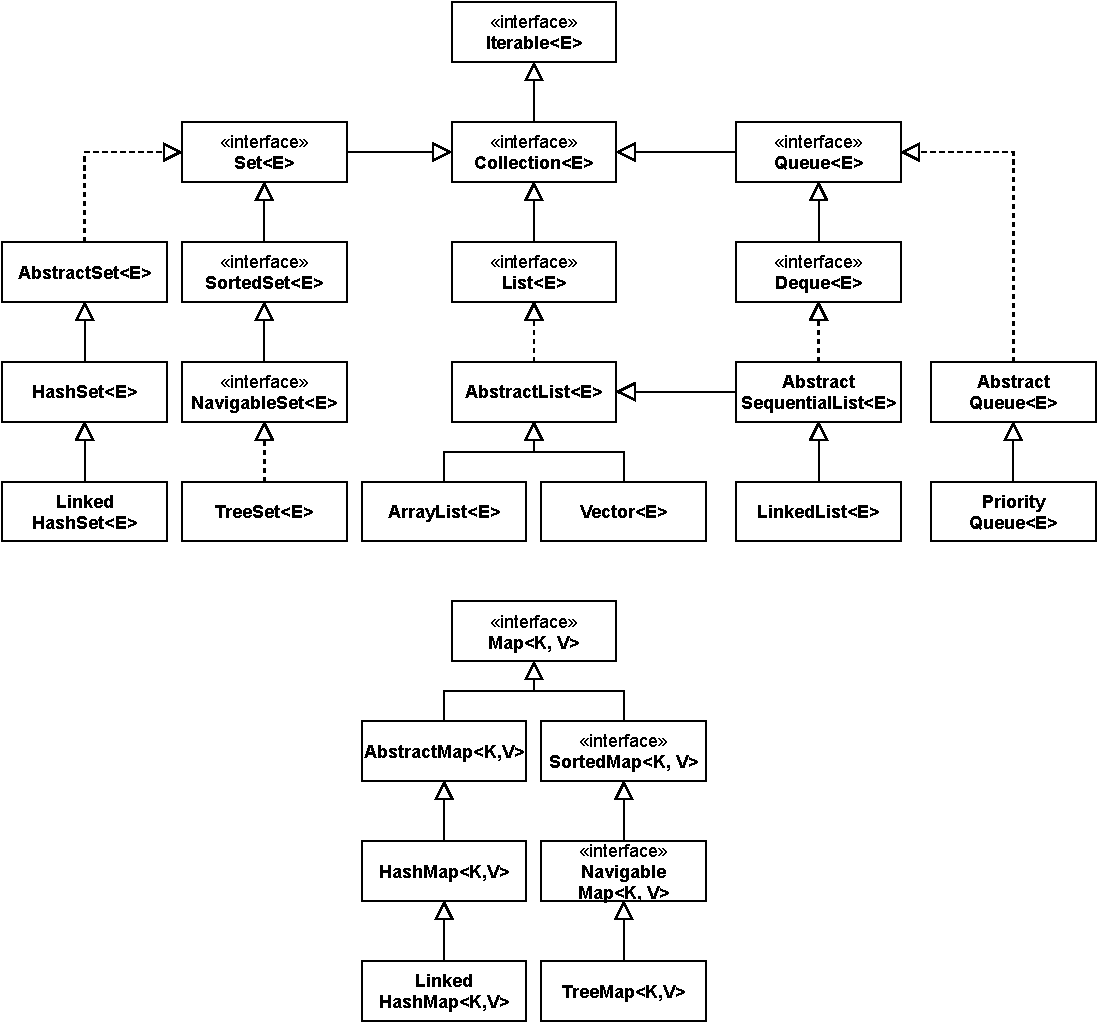
\includegraphics[width=.9\linewidth]{java-collections}
    \caption{Allerlei verschillende generic collection interfaces en classes van de Java Collections API.}
    \label{fig:java-collections}
\end{figure}

Elke soort collectie heeft zijn eigen doel. 
Om bijvoorbeeld een lijst van shapes aan te geven, 
kan je verwijzen naar \texttt{List<Shape2D>} (\textit{a list of shapes})
en deze invullen met een ArrayList<Shape2D> implementatie.
Waar lijsten echter vooral zijn bedoeld om elementen aan te bieden op een bepaalde volgorde,
gebruiken we sets vooral om bij te houden of we iets gezien hebben of niet. Een element 
kan maar één keer in een set zitten en een set bevat handige operaties om set logica 
uit te voeren. Een set van namen kan bijvoorbeeld weergegeven worden als 
\texttt{Set<Name>} (\textit{a set of names}).
Een map is bedoeld als een doorzoekbaar register (een dictionary),
waarbij een \textit{key} van een bepaald type kan verwijzen naar 
een \textit{value} van een bepaald ander type. Stel dat we bijvoorbeeld
willen bijhouden hoe vaak een bepaalde naam voorkomt in een groep,
dan kunnen we een \texttt{Map<Name, Integer>} (\textit{a map of names to integers})
bijhouden.

In dit geval zijn de List, Set en Map allemaal generic interfaces en
worden de type arguments ingevuld door Shape2D, Name en Integer.
Maar hoe definieer je een generic type? Laten we eens kijken naar de 
een deel van de Map-interface, zoals deze in Java is gedefinieerd,
zie Voorbeeld~\ref{code:map-generic}.

\begin{listing}[H]
\begin{minted}[linenos]{java}
public interface Map<K, V> {
    V put(K key, V value);
    V get(Object key);
    // Much more methods...
}
\end{minted}
\caption{Een deel van de generic Map-interface zoals deze is opgenomen in Java.}
\label{code:map-generic}
\end{listing}

In Voorbeeld~\ref{code:map-generic} zien we dat twee type arguments:
K en V. Deze types kunnen later worden ingevuld voor de elementen die 
als respectievelijk \textit{key} en \textit{value} worden opgenomen in de Map.
Je kan in een map dus een object van het ene type laten wijzen naar een 
object van het andere type 
(bijvoorbeeld een String naar een Integer, of een FullName naar een Address).

\subsection{Functional interfaces, streams, lambda expressions}
Sinds Java 8 kunnen we functies gebruiken als object. Dit zijn speciale objecten 
die een \textit{functional interface} implementeren. Je kan 
een functie declareren als variabele, teruggeven uit een methode of gebruiken 
als parameter. Dit maakt het makkelijker om bepaald gedrag mee te geven en 
te variëren aan een bestaande datastructuur. Dit klinkt nogal ingewikkeld en het 
is even wennen, maar je kan er een boel mee!

Een plek waar dit soort functies met name veel gebruikt worden is door een 
specifieke operatie uit te voeren op de elementen in een verzameling, bijvoorbeeld
het berekenen van de som van alle getallen in een lijst 
het aanpassen van alle waarden in een set of 
het filteren van bepaalde element uit een verzameling.
Hiervoor kan je sinds Java 8 gebruik maken van de \textit{Streams API}.
Op een verzameling in Java kan je \texttt{.stream()} aanroepen en vervolgens 
een methode die een functional interface verwacht. Een \texttt{Stream<T>} is 
een generiek type waarbij de elementen worden aangeboden als een reeks waarden over tijd.

Neem bijvoorbeeld een methode om uit een lijst van namen (\texttt{List<String>}),
de namen te verzamelen die beginnen met een bepaalde letter of reeks letters.
Met een for-loop zouden we dat bijvoorbeeld als volgt doen (Figuur~\ref{code:filter-loop}):

\begin{listing}[H]
\begin{minted}[linenos]{java}
public class FriendsList {
    private List<String> names = 
        List.of("Alex", "Bert", "Arnold", "Anton");

    public List<String> selectNamesByPrefix(String prefix) {
        List<String> selection = new ArrayList<>();

        for (String name : names) {
            String lowerCaseName = name.toLowerCase();
            if (lowerCaseName.startsWith(prefix)) {
                selection.add(name);
            }
        }

        return selection;
    }
}
\end{minted}
\caption{Het selecteren van namen op basis van een bepaalde prefix met behulp van een loop.}
\label{code:filter-loop}
\end{listing}

Als we gebruik maken van de Streams API ziet dezelfde method eruit als in Figuur~\ref{code:filter-streams}.

\begin{listing}[H]
\begin{minted}[linenos]{java}
public class FriendsList {
    private List<String> names = 
        List.of("Alex", "Bert", "Arnold", "Anton");

    public List<String> selectNamesByPrefix(String prefix) {
        return names.stream()
            .map(name -> name.toLowerCase())
            .filter(name -> name.startsWith(prefix))
            .collect(Collectors.toList());
    }
}
\end{minted}
\caption{Het selecteren van namen op basis van een bepaalde prefix met behulp van de Streams API.}
\label{code:filter-loop}
\end{listing}

Met \texttt{.stream()} veranderen we de lijst in een stream, zodat we er 
stream-operaties op kunnen uitvoeren.
Aan de \texttt{map} en \texttt{filter} methodes kunnen we een functie meegeven.
In het geval van de map-methode is het een functie die een String transformeert 
naar een andere String (\texttt{Function<String, String>}). In het geval 
van de filter-methode is geven we een predicate mee (\texttt{Predicate<String>}). 
Dit is een functie die een boolean teruggeeft op basis van een bepaalde invoer, in ons geval een String.
De filter-methode selecteert elementen op basis van de meegegeven predicate function.
Ten slotte moeten we de Stream weer omzetten naar een lijst, dat doen we met een \texttt{Collector}.

De pijlfunctie die we meegeven aan een stream-operatie noem je een \textit{lambda expressie} of \textit{arrow function}.
Dit een verkorte manier om een functie te declareren. De compiler check wel of het een verwachte en kloppende
implementatie oplevert van een functional interface.
Soms kan, in plaats van een lambda expressie, ook verwijzen naar een methode op een bepaalde instantie door naar diens naam 
op de klasse te wijzen. In het voorbeeld zouden we \texttt{name -> name.toLowerCase()} kunnen vervangen 
met \texttt{String::toLowerCase}.

Er zijn een boel verschillende stream-operaties en hoop verschillende soorten functional interfaces.
Het is ook mogelijk om zelf functional interfaces te declareren. Dat gaat te ver voor nu.

\subsection{Optionals}
In Java 8 is het generieke type van de \textit{Optional<T>} toegevoegd aan de taal.
De \texttt{T} is een \textit{type argument} dat door de developer zelf ingevuld kan worden.
Optionals zijn bedoeld als alternatief voor \texttt{null} en het voorkomen van 
\texttt{NullPointerException}s. Deze foutmelding krijg je bijvoorbeeld wanneer 
je een methode of veld op \texttt{null} probeert aan te roepen. Vaak gebeurt dit 
wanneer je uit een opslag iets probeert op te vragen dat er niet is. De standaardoplossing
hiervoor is om overal waar je \texttt{null} kan verwachten te checken of 
er sprake is van \texttt{null} of niet. Helaas kan onze compiler niet goed statisch (tijdens compilatie)
bepalen of we voldoende hebben gecheckt of we null terug kunnen krijgen.
Optional probeert daarbij te helpen en voegt daarnaast
wat methoden toe die de code simpeler kunnen maken.

Stel we hebben een methode die \texttt{Optional<User>} teruggeeft. Dan krijgen we 
een Optional-object terug, waarin een User \textit{kan} zitten. Dat hoeft niet zo 
te zijn. Door Optional als type te gebruiken (in plaats van \texttt{null} terug te geven),
kunnen compiler en IDE gemakkelijker waarschuwen als we vergeten om te checken of 
er wel daadwerkelijk een waarde terug wordt gegeven.

Het handige aan Optionals zijn de methodes die code een stukje simpeler kunnen maken.
Voor \texttt{Optional<User>} kunnen we de methodes aanroepen als in Tabel~\ref{table:optional-methods}.

\begin{table}[H]
    \centering
    \begin{tabularx}{\textwidth}{
        |>{\raggedright}l|>{\raggedright}X|>{\raggedright\arraybackslash}X|
    }
    \hline
    \textbf{Methode} 
    & \textbf{Return type} 
    & \textbf{Beschrijving} 
    \\ \hline
        
    \texttt{isPresent}
    & \texttt{boolean}
    & Geeft terug of er een waarde in de optional zit of niet.
    \\ \hline

    \texttt{ifPresent}
    & \texttt{void}
    & Voert de meegeven \textit{consumer function} uit als er een waarde inzit, maar 
    doet niets als deze leeg is.
    \\ \hline

    \texttt{orElse}
    & \texttt{User}
    & Geeft de ingesloten User terug of de aangegeven default User als de optional leeg is.
    \\ \hline

    \texttt{orElseThrow}
    & \texttt{User}
    & Geeft de ingesloten User terug of gooit een exception als de optional leeg is.
    \\ \hline

    \texttt{get}
    & \texttt{User} (gooit een \texttt{NoSuchElementException} als leeg)
    & Met deze methode kan je de waarde uit de Optional halen. 
    Dit kan je eigenlijk alleen doen als je weet dat de Optional een waarde bevat. 
    \\ \hline

    \end{tabularx}
    \caption{Een aantal methods voor \texttt{Optional<User>}, in variabele \texttt{optionalUser}.
    Dit is generiek toepasbaar op elk soort \texttt{Optional<T>}.}
    \label{table:optional-methods}
    \centering
\end{table}

Een voorbeeld van het gebruik van \texttt{Optional} is te vinden in de ChipsService
die aan de ChipsRepository het aantal Chips voor de gebruiker opvraagt. Zie Voorbeeld~\ref{code:chips-optional}
Als er geen chips voor de gebruiker gevonden kunnen worden, wordt standaard een Chips-object teruggegeven met een waarde van 0.
Afhankelijk van hoe strikt je je foutafhandeling wil inrichten,
zou je hier als alternatief een exception kunnen gooien met \texttt{.orThrow}.

\begin{listing}[H]
\begin{minted}[linenos]{java}
public Chips findChipsByUsername(String username) {
    return this.chipsRepository
            .findByUsername(username)
            .orElse(new Chips(username, 0L));
}
\end{minted}
\caption{We gebruiken een Optional om 0 chips terug te geven als er geen chips voor de gebruiker gevonden kunnen worden.}
\label{code:chips-optional}
\end{listing}

\section{Annotations}
Sinds JDK 1.6 kennen we \textit{annotaties} in Java. 
Dit is een manier om metadata toe te voegen aan klassen,
methodes, velden en parameters. Met annotaties kan je 
data of gedrag toevoegen aan een element door deze erboven te 
zetten. Een annotatie ziet eruit als een klassenaam met een apenstaartje ervoor.

Annotations worden erg veel gebruikt in frameworks. Bijvoorbeeld
om een datamodel te declareren met Hibernate (\texttt{@Entity})
of om aan te geven dat een bepaalde klasse als een injecteerbare 
service moet worden gezien in Spring (\texttt{@Service}).

Een annotatie kan ook een instructie aan de compiler zijn.
Bij het implementeren van een interface of het overerven van een klasse 
kan je in de subklasse boven de overschreven of geïmplementeerde methode 
de annotatie \texttt{@Override}. De compiler checkt dan of de betreffende
methode wel daadwerkelijk een overschrijving is van een bestaande methode,
dus op de parent(s) aanwezig was. Dit biedt een extra laag bescherming tegen 
programmeerfouten.

\section{Exceptions}
\textit{Exceptions} zijn bedoeld om de reguliere programmaflow
te doorbreken in het geval van een fout. Zodra de fout plaatsvindt, 
stopt de uitvoering van een bepaalde functie en moet de fout worden afgehandeld.
Gebeurt dat niet in de methode waar de exception gegooid wordt, dan wordt gekeken 
of het in de methode gebeurt die die methode aanroept. Is er geen methode waarin 
de exception wordt afgehandeld, dan crasht het programma en laat Java een 
\textit{stack trace} zien.

\subsection{Try, throw en catch}
Om aan te geven dat er iets gebeurt dat niet mag of niet verwacht wordt, kunnen we een
exception \textit{gooien} (\texttt{throw}). Zie Voorbeeld~\ref{code:chips-throw}.
Bij het opnemen van Chips in ons casinoproject willen we niet dat iemand 
een negatief getal kan opnemen of teveel chips kan opnemen. Daarom gooien we in 
het Chips-object een exception als niet aan de voorwaarden wordt voldaan! 

\begin{listing}[H]
\begin{minted}[linenos]{java}
public void withdraw(Long amountToWithdraw) {
    if (amountToWithdraw < 0) {
        throw new NegativeNumberException(
            "Cannot withdraw a negative amount: " + amountToWithdraw
        );
    }

    long newAmount = this.amount - amountToWithdraw;
    if (newAmount < 0) {
        throw new NotEnoughChipsException(
                String.format(
                        "Cannot withdraw %d chips: %d chips remaining",
                        amountToWithdraw,
                        this.amount
                )
        );
    }

    this.amount = newAmount;
}
\end{minted}
\caption{We gooien een exception in het Chips-object als iemand een negatief aantal chips 
wil opnemen of als er teveel chips worden opgenomen.}
\label{code:chips-throw}
\end{listing}

De betreffende exception kan op hetzelfde 
of op een hoger niveau worden \textit{opgevangen} (\texttt{catch}) en worden afgehandeld.
Het gedeelte waar we een exception kunnen verwachten, stoppen we in een \texttt{try}-blok,
wat we afsluiten met een \texttt{catch}-aanduiding.

In het geval van de Chips wordt deze foutmelding niet in het Chips-object,
niet in de ChipsService, maar in de ChipsController afgehandeld en omzet naar 
de juiste HTTP-statuscode. Het Spring framework helpt hierbij: 
de \texttt{ResponseStatusException} wordt automatisch omgezet naar een HTTP-response met 
de meegegeven HTTP-statuscode. Status codes zijn voor clients van belang om te bepalen 
met wat voor een soort foutmelding we te maken hebben.

\begin{listing}[H]
\begin{minted}[linenos]{java}
@PostMapping("/withdraw")
public Balance withdraw(
    Authentication authentication, 
    @Validated @RequestBody Withdrawal withdrawal
) {
    UserProfile profile = (UserProfile) authentication.getPrincipal();

    try {
        Balance balance = this.service.withdrawChips(
            profile.getUsername(), 
            withdrawal.amount
        );
        return balance;
    } catch (NotEnoughChipsException exception) {
        throw new ResponseStatusException(
            HttpStatus.PAYMENT_REQUIRED, 
            exception.getMessage()
        );
    } catch (NegativeNumberException exception) {
        throw new ResponseStatusException(
            HttpStatus.BAD_REQUEST, 
            exception.getMessage()
        );
    }
}
\end{minted}
\caption{In de Chips-controller wordt de exception afgehandeld 
en omgezet naar de juiste statuscode met behulp van het Spring framework.}
\label{code:chips-throw}
\end{listing}

Het kan zijn dat we na het afhandelen van de exception nog wat willen uitvoeren,
bijvoorbeeld wanneer er bepaalde operaties moeten worden teruggedraaid of een bestand 
moet worden verwijderd. In dat soort situaties kunnen we \texttt{finally} gebruiken.

\subsection{Checked versus unchecked}
In Java kennen we twee verschillende soorten exceptions: 
checked exceptions en unchecked exceptions.
\textit{Checked exceptions} zijn exceptions waarbij de compiler 
\texit{checkt} of ze in de methode die ze kunnen veroorzaken worden afgehandeld.
Als dat niet zo is, moet in de method signature worden opgenomen dat deze 
een exception kan gooien, door \texttt{throws} op te nemen na de methodelijst.
De methode waarin de `gooiende' methode wordt aangeroepen speelt het vervolgens weer:
afhandelen of aangeven in de method signature. Aan de ene kant geven checked exceptions 
dus wat meer betrouwbaarheid dat fouten daadwerkelijk worden afgehandeld. Aan de andere kant 
zorgt dit voor een boel extra code, terwijl je vaak de foutafhandeling wil verplaatsen 
naar de randen van je applicatie als je niet meteen van de fout kan herstellen. 
In dat soort situaties gaat het meestal om de omzetting van een onduidelijke exception 
naar een voor programmeurs (en gebruikers) leesbare foutmelding. Zodat helder is 
wat er precies fout is gegaan en of het aan de gebruiker of de software ligt.

Bij \textit{unchecked exceptions} voert de compiler niet zo'n controle uit.
Dan is het dus aan de programmeur om goed na te denken hoe met een dergelijke 
fout wordt omgegaan. In frameworks, zoals Spring, wordt een algemene exception handler 
gebruikt. Als een gebruiker een fout in de uitvoering veroorzaakt en de programmeur heeft 
dit niet afgehandeld, dan wordt dit standaard afgehandeld door Spring. In plaats van dat 
de hele applicatie crasht, krijgt alleen het specifieke verzoek van deze gebruiker een foutmelding
terug. In termen van het web zal dit standaard een \texttt{500 Server Error} zijn.

\subsection{Custom exceptions}
Natuurlijk kent Java een aantal standaardexceptions om verschillende foutscenario's aan te geven.
Het is echter vaak handig om eigen exceptions te definiëren. Op die manier kan je net wat meer 
context meegeven en kan je in de code duidelijk zien om welke foutmelding het gaat. 

In het geval van het opnemen van Chips hebben we twee custom exceptions gemaakt: 
\texttt{NegativeNumberException} en \texttt{NotEnoughChipsException}. 
Dit zijn subtypes van RuntimeException, de basisexception voor alle 
unchecked exceptions in Java. We hebben slechts één constructor gemaakt, 
waarin de message wordt doorgegeven naar de superklasse. 
Zie Voorbeeld~\ref{code:chips-custom-exception}.
Natuurlijk kan je veel meer methodes toevoegen. Soms loont het om een named constructor 
op te nemen die in detail beschrijft wat er precies is fout gegaan.

\begin{listing}[H]
\begin{minted}[linenos]{java}
// NotEnoughChipsException.java
public class NotEnoughChipsException extends RuntimeException {
    public NotEnoughChipsException(String message) {
        super(message);
    }
}

// NegativeNumberException.java
public class NegativeNumberException extends RuntimeException {
    public NegativeNumberException(String message) {
        super(message);
    }
}
\end{minted}
\caption{We maken custom exceptions door een exception-klasse van Java te extenden.}
\label{code:chips-custom-exception}
\end{listing}

\chapter{Object-oriëntatie}
We hebben het al gehad over object-georiënteerd programmeren
in Java, maar wat zijn precies de ideeën hierachter?
Hoe kunnen we objecten inzetten om separation of concerns,
loose coupling en high cohesion te bereiken?

Hiervoor is het zinvol om stil te staan bij de algemene eigenschappen 
zijn object-oriëntatie. We sluiten hierbij aan 
bij het objectmodel uit het boek 
Object-Oriented Analysis and Design with Applications 
van object- en UML-pionier Grady Booch en anderen. 
Hierin staan een aantal belangrijke en minder belangrijke 
elementen die in object-georiënteerde projecten voorkomen. 
Deze elementen kan je ook tegenkomen bij andere stijlen van programmeren,
maar wij staan vooral stil bij hoe deze elementen gebruikt kunnen worden 
in een object-georiënteerde taal. Hoe kunnen we deze elementen benutten 
om tot een sterk ontwerp te komen?

\section{Het objectmodel van Booch}
Het objectmodel van Booch onderscheidt vier belangrijke elementen 
die een rol spelen bij het object-georiënteerd modelleren:
\footnote{
    In de praktijk wordt ook wel eens verwezen naar de \texit{4 Pillars of Object Orientation}: 
    abstraction, encapsulation, polymorphism en inheritance. 
    Deze zijn in het objectmodel van Booch inbegrepen.
}
\begin{enumerate}
    \item Abstraction
    \item Encapsulation 
    \item Modularity 
    \item Hierarchy
\end{enumerate}

Deze onderdelen noemen Booch et al. belangrijk omdat je 
zonder deze elementen geen object-georiënteerde taal (OO-taal) kan hebben.
Daarnaast beschrijven zij drie minder belangrijke elementen die je 
bij veel OO-talen tegen kunt komen: typing, persistence en concurrency.

Dit betekent natuurlijk niet dat je deze zaken buiten OO-talen niet tegen zal komen! 

\subsection{Abstraction}
In een object-georiënteerde taal zijn objecten de abstracties 
waarmee we werken. Het is niet de bedoeling van een abstractie 
om de wereld precies na te bootsen.
We willen concepten modelleren voor zover deze van belang zijn 
voor het domein van de applicatie en het betreffende programmaonderdeel.
In een object zijn toestand (fields) en gedrag (methods) samengebracht
om een bepaalde rol binnen een systeem te vervullen.

\blockquote{
    An abstraction denotes the essential characteristics 
    of an object that distinguish it from all other kinds 
    of objects and thus provide crisply defined conceptual
    boundaries, relative to the perspective of the viewer.
}{\cite{Booch2007}, p. 44.}

Een manier om te kijken naar abstractie is door 
het object te beschouwen van de buitenkant. 
We zien manieren om met het object te interacteren,
maar we kunnen niet naar binnen kijken of invloed 
uitoefenen op de interne structuur of hoe het object
precies omgaat met die interactie.
\cite{Abelson1996} noemen dit een \textit{abstraction barrier}
 in hoofdstuk 2 van het invloedrijke boek 
Structure en Interpretation of Computer Programs.
Als gebruiker van een object kunnen we alleen maar 
zien tot de "grens" van een abstractie en niet daar voorbij.
We kunnen alleen interacteren met het protocol (de API) van 
het object: diens publieke method signatures.
In Java en veel andere talen kan je dit protocol afdwingen
met behulp van \textit{interfaces}. De interne implementatie 
van een object is dus verborgen. 
Dit noemt men ook wel \textit{implementation hiding}.

Liskov en Zilles beschreven in hun zoektocht naar 
programmeren met abstracties een dergelijke grens:
\blockquote{
    When a programmer makes use of an abstract data object,
    he is concerned only with the behavior which 
    that object exhibits but not with any details of how that 
    behavior is achieved by means of an implementation.
    The behavior of an object is captured by the set of 
    characterizing operations.
    \newline\newline
    (...)
    \newline\newline
    Implementation information (...)
    is only needed when defining how the characterizing 
    operations are to be implemented.
    The user of the object is not required to know 
    or supply this information.
}{\cite{Liskov1974}, p. 51.}

Het voordeel van het werken met abstracties is dus 
dat we ons niet bezig hoeven te houden met de precieze
interne werking van een object, maar als buitenstaanders 
ons slechts hoeven te concentreren op de aangebode publieke 
methodes. 

Bij een digitaal kaart- of bordspel zou je een abstractie kunnen 
aanmaken voor het spelpotje zelf, zodat de gehele speltoestand 
opgeslagen kan worden. Acties die door de speler(s) op het spel 
kunnen worden uitgevoerd kunnen dan opgenomen worden als methodes
op het spelpotje. De verschillende onderdelen en concepten binnen 
het spel zou je kunnen opnemen als aparte objecten met hun eigen 
velden, methodes en regels. Concepten die in het spel voorkomen 
kunnen gemodelleerd worden als objecten die op hun beurt weer 
van slimme, beschrijvende methodes kunnen worden voorzien. 
Denk bijvoorbeeld aan een object 
waar bepaalde spelregels in zijn opgenomen, aan alles wat je binnen 
een spel met een kaart kan doen of bijvoorbeeld het onderscheid tussen 
een pakje kaarten en een hand met kaarten. Elke abstractie heeft zijn 
eigen toestand en gedrag. Met een beetje goede naamgeving leest 
de code dan ook als een samenvatting van spelacties!

Met abstraction kunnen we cohesion verhogen door zaken 
bij elkaar te stoppen die bij elkaar 
horen en koppeling verminderen door afhankelijk te zijn van de 
API van een object in plaats van diens interne implementatiedetails.

\subsection{Encapsulation}
Encapsulation and abstraction zijn twee kanten van dezelfde 
medaille. Abstraction is een perpectief van buitenaf: 
wat voor interactiemogelijkheden biedt een object 
en hoe gedraagt dit object zich?
\textit{Encapsulation} (of: inkapseling) 
richt zich meer op de binnenkant:
hoe wordt het interne gedrag afgeschermd van de 
buitenwereld? Object-georiënteerde code benut 
encapsulation op koppeling te reduceren.

\blockquote{Encapsulation is the process 
of compartmentalizing the elements of an 
abstraction that constitute its structure and 
behavior; encapsulation serves to separate the
contractual interface of an abstraction and its 
implementation.}{\cite{Booch2007}, p. 52.}

\textit{Information hiding} speelt hierbij een belangrijke 
rol: we willen niet hebben dat elk object bij elkaars 
interne datastructuren kan komen. In plaats daarvan 
willen we controle uitoefenen over de afhankelijkheden.
Door informatie te verbergen kan je namelijk het aantal 
en de ingrijpendheid van afhankelijkheden tussen 
klassen verminderen. Hiervoor gebruiken we in Java
de access modifier \textit{private}.
Het moderne begrip van encapsulation is gebaseerd op 
Parnas-modules, genoemd naar David Parnas.
Hij beschreef afhankelijkheden als \emph{connections}
en vond dat connecties niet teveel informatie mochten prijsgeven.
\blockquote{
    The connections between modules are the assumptions
    which the modules make about each other.
    \newline\newline
    (...)
    \newline\newline
    We ask, ``What changes can be made to one module
    without involving change to other modules?'' 
    We may make only those changes which do not violate
    the module being changed. In other words,
    a single module may be changed only while the `connections'
    still `fit'. Here, too, we have a strong argument for
    for making the connections contain as little information as possible.
}{\cite{Parnas1971}, pp. 339-340}

Encapsulation, in het bijzonder information hiding,
kan dus helpen om het aantal afhankelijkheden te reduceren
en dus koppeling te verlagen. 

We hebben als het ware een \textit{capsule}
waarbinnen de kern van heb object ligt besloten en kunnen alleen met die 
capsule praten via de publieke methoden. Om die reden willen we voorzichtig
zijn met het \texttt{public} maken van fields of het standaard toevoegen van 
getters en setters. Dit vergroot de kans dat buitenstaande objecten gekoppeld 
raken aan de interne structuur van een object. Door alleen te koppelen tegen 
de publieke methodes van een object, is het makkelijker om de interne toestand 
van het object te wijzigen.

\subsubsection{Tell, Don't Ask}
Een algemene vuistregel om het gebruik van getters en setters te verminderen,
is \textit{Tell, don't ask}. Hiermee wordt bedoeld dat je liever tegen een object 
wil zeggen wat het moet doen, in plaats van dat je alle informatie eruit trekt
er wat mee doet en het vervolgens weer terug in het object stopt. 
Dit wordt wat versimpeld weergegeven in Voorbeeld~\ref{code:tell-dont-ask}.
In de echte wereld zou je natuurlijk liever de geboortedatum van de persoon 
opslaan en heb je dit probleem niet.

\begin{listing}[H]
\begin{minted}[linenos]{java}
String name = "Alex";
Integer age = 31;
Person person = new Person(name, age);

// Don't make a "dumb" object...
Integer afterBirthday = person.getAge() + 1;
person.setAge(afterBirthday);

// Rather, let the object do the work!
person.celebrateBirthday();
\end{minted}
\caption{\textit{Tell, don't ask} houdt in dat je het object het werk laat doen.
Bijkomstig voordeel is dat de bedoeling van de actie duidelijk wordt.}
\label{code:tell-dont-ask}
\end{listing}

Op deze manier reduceer je niet alleen de koppeling, 
je maakt een object meer samenhangend omdat de logica 
die hoort bij wat het betreffende object vertegenwoordigt
onderdeel is van het object. Het hoort bij diens verantwoordelijkheid.
Je kan een boel versimpelen door minder met getters en setters te werken!

\subsubsection{Law of Demeter}
De \textit{Law of Demeter} of \textit{the principle of least knowledge} 
is een extra richtlijn om encapsulation in te richten en koppeling te reduceren
(\cite{Lieberherr1989}). In de praktijk wordt dit vaak als volgt samengevat:

\begin{itemize}
    \item Objecten mogen slechts kennis hebben van andere objecten als ze nauw eraan verwant zijn
    \item Objecten mogen alleen praten met vrienden, niet met vreemden
    \item Objecten mogen alleen praten met directe vrienden, niet met vrienden van vrienden
\end{itemize}

Probeer objecten dus alleen met elkaar te laten praten als ze 
structureel met elkaar samenhangen of als ze een duidelijke dienst afnemen.
Als het gaat om een dienst, praat dan met het object dat de dienst verleent 
en ga niet met de objecten praten die dat dienstverlendende object gebruikt om
de dienst te vervullen. 
In andere woorden: koppel niet tegen de interne representatie van een object!

Helaas werken veel object-georiënteerde projecten niet volgens dit principe en 
is de code met getters in elkaar geknoopt. 
Zo koppel je buitenstaande objecten niet alleen op de 
interne toestand van één object, maar op de interne toestanden van 
de objecten die daarin liggen besloten. Zie Voorbeeld~\ref{code:train-wreck}.

\begin{listing}[H]
\begin{minted}[linenos]{java}
// A client class, for example: Main.java
Result result;
Integer player1Score = game.getCurrentRound().getPlayer1().getScore();
Integer player2Score = game.getCurrentRound().getPlayer2().getScore();

if (player1Score > player2Score) {
    result = Result.PLAYER_ONE_WON;
} else if (player2Score > player1Score) {
    result = Result.PLAYER_TWO_WON;
} else {
    result = Result.DRAW;
}
\end{minted}
\caption{Dit is een \textit{train wreck} en een overtreding van \textit{the Law of Demeter}.
We moeten namelijk de innerlijke structuur van \texttt{Game}, \texttt{Round} en \texttt{Player} weten.
Dit introduceert meer coupling dan noodzakelijk!}
\label{code:train-wreck}
\end{listing}

Dit is wat men ook wel een 
\textit{train wreck} noemt, omdat de method calls achterelkaar een soort 
treintje met wagonnetjes vormen (\texttt{game.getCurrentRound().getPlayer1().getScore()}).

Om dit tegen te gaan, kan je \textit{Tell, don't ask} toepassen 
om encapsulation te bereiken en te koppelen tegen de abstractie: 
vertel de objecten wat ze moeten doen, in plaats van alle data eruit te trekken.
De externe coupling is dan kleiner, omdat we de interne cohesie benutten.

\begin{listing}[H]
\begin{minted}[linenos]{java}
// A client class, for example: Main.java
Result result = game.evaluateCurrentRound();

// Inside Game.java:
public Result evaluateCurrentRound() {
    // getCurrentRound is a private method
    Round round = this.getCurrentRound();
    return round.evaluate();
}

// Inside Round.java:
public Result evaluate() {
    if (player1.scoredHigherThan(player2)) {
        return Result.PLAYER_ONE_WON;
    } else if (player2.scoredHigherThan(player1)) {
        return Result.PLAYER_TWO_WON;
    } else {
        return Result.DRAW;
    }
}

// Inside Player.java:
public Boolean scoredHigherThan(Player other) {
    // Note: instances can access private fields of other instances of the same class
    return this.score > other.score;
}

\end{minted}
\caption{We reduceren de coupling van buitenaf door meer gebruik te maken van de 
kracht van samenhangende, doelgerichte objecten.}
\label{code:train-wreck-solution}
\end{listing}

In sommige gevallen ontkom je niet aan het gebruik maken van getters.
Dit is vaak het geval bij \textit{serializatie} van objecten naar een ander formaat.
Denk bijvoorbeeld aan het omzetten van een object naar een JSON-representatie 
of naar een SQL-query. Omdat dit gewoonlijk aan de randen van je applicatie gebeurt,
wordt hiervoor vaak \textit{data transfer objects (DTOs)} voor ingezet.

\subsection{Modularity}
Volgens \cite{Booch2007} zijn object-georiënteerde projecten
onderhoudbaar ingericht dankzij \textit{modularity}.

\blockquote{
    Modularity is the property of a system
    that has been decomposed into a set
    of cohesive and loosely coupled modules.    
}{\cite{Booch2007}, p. 56.}

Klassen, packages en interfaces zijn de belangrijkste modules binnen 
een object-georiënteerd project. Zie hierover uitgebreid het hoofdstuk 
over object-georiënteerd programmeren in Java.

In Java brengen we toestand (fields) en gedrag (methods) samen 
in klassen en kunnen we klassen groeperen middels packages.
Interfaces kunnen helpen om, dankzij polymorfisme, abstractie en 
implementatie van elkaar te scheiden en zodoende programmaonderdelen 
van elkaar los te koppelen. Met enums kunnen we het aantal mogelijkheden 
beperken. Generics helpen ons om (geparameterizeerde) containertypen te 
maken waarvan de interne types kunnen variëren dankzij type arguments.
Deze modules helpen ons een \textit{separation of concerns} te bereiken.

\subsection{Hierarchy}
Hiërarchie is een ander element van het werken met objecten om een 
project onderhoudbaar te houden.

\blockquote{
    Hierarchy is a ranking or ordering of abstractions.
}{\cite{Booch2007}, p. 58.}

Met de juiste naamgeving en een intelligente package structuur 
kunnen we een onderhoudbare \textit{softwarearchitectuur} opzetten, waarin 
packages een rol van betekenis vervullen. We brengen daarmee een 
hiërarchie aan in ons softwareproject: een bewuste rangschikking van waar welke 
packages te vinden zijn.

Binnen het domein kunnen we ook een objecthiërarchie waarnemen:
vaak hebben we één object die verantwoordelijk is voor het uitvoeren van 
de domeinacties. Meestal bestaat dit object weer uit allemaal andere objecten
die elk hun eigen velden, methodes en regels bevatten. Op die manier blijft 
niet alleen de code overzichtelijk en kan je onderdelen uitwisselen, de code 
kan soms lezen als een natuurgetrouwe weergave van acties --- met hier en daar 
wat Java-syntax ertussen.

Laten we wat dieper ingaan op deze objecthiërarchie. 
Objecten en klassen staan namelijk niet op zichzelf.
Ze vertonen allerlei relaties tot elkaar. In de meest algemene 
zin kan een object kan een ander object gebruiken (\textit{afhankelijkheid}).
Dit algemene gebruik kan verder worden gespecifieerd. Een object kan 
bijvoorbeeld zijn opgebouwd uit andere objecten (\textit{associatie, aggregatie, compositie}).
Ook kan een klasse een interface implementeren (\textit{realisatie}) of
van een andere klasse fields en methods overerven (\textit{overerving}).
Laten we deze dependency types nader onderzoeken aan de hand 
van de Unified Modeling Language (UML), zoals genoemd in \cite{Booch1999}.

\subsubsection{Afhankelijkheid (`gebruikt')}
Een \textit{afhankelijkheid} (\textit{dependency}) geeft aan dat 
de werking van een bepaalde module op de een of andere manier afhangt
van een andere module. We zeggen ook wel dat de ene module de andere 
module gebruikt.

\blockquote{
    A dependency is a using relationship that states
    that a change in specification of one thing (...)
    may affect another thing that uses it, 
    but not necessarily the reverse.    
}{\cite{Booch1999}, p. 63.}

Zie bijvoorbeeld de withdrawChips-methode in de ChipsService 
van het chips-component het casinoproject (Voorbeeld~\ref{code:withdraw-chips}). 
We halen een Chips-object op uit de ChipsRepository 
via \texttt{this.findChipsByUsername(username)}).
Onze ChipsService \textit{gebruikt} dus de Chips-klasse!

\begin{listing}[H]
\begin{minted}[linenos]{java}
public Balance withdrawChips(String username, Long amount) {
    Chips chips = this.findChipsByUsername(username);

    chips.withdraw(amount);
    this.chipsRepository.save(chips);

    return this.showBalanceFor(chips);
}
\end{minted}
\caption{De \texttt{withdrawChips}-methode uit de ChipsService.}
\label{code:withdraw-chips}
\end{listing}

In een UML-klassediagram zouden we dat (versimpeld) weergeven 
als in Figuur~\ref{fig:uml-dependency}.

\begin{figure}[H]
    \centering
    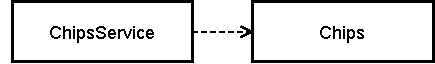
\includegraphics[width=.6\linewidth]{uml-dependency}
    \caption{ChipsService gebruikt de Chips-klasse}
    \label{fig:uml-dependency}
\end{figure}

Je modelleert een relatie als een algemene afhankelijkheid 
als je niet verder kunt of hoeft te specificeren om wat 
voor een soort afhankelijkheid het gaat. Het is vaak wel 
aan te raden om wat dieper te kijken naar het soort relatie
dat de afhankelijkheid vormt.

\subsubsection{Associatie (`zit vast aan')}
Een \textit{associatie} is een algemene manier om te beschrijven dat een 
bepaald object structureel verbonden is met een ander object.
Dit betekent dat het ene object, of een referentie daaraan, 
op de een of andere manier opgenomen is in het andere object.
Dit zie je meestal terug als een \textit{field declaration}
in de klasse. In UML neem je de association echter niet 
op in de klasse, maar wordt deze vertegenwoordigt door een 
lijn of een pijl. Bij een associatie geef je de rolnaam en de 
multipliciteit aan. Een rolnaam komt doorgaans overeen met 
de \textit{field name} en de multipliciteit is een bereik 
van 0 tot 1, 0 tot meer of 1 tot meer. We geven een 
multipliciteitswaarde van "tot meer" aan als het veld is 
gedefinieerd als een collectie.
Een multipliciteitswaarde kan 0 
zijn als de structurele verbinding optioneel is. Dit is het 
geval wanneer het veld conceptueel \texttt{null} mag zijn. 
Naast deze bereiken kan het voorkomen dat een associatie 
exact 1 keer is gevuld.

Een associatie geef je in UML aan met een reguliere pijl om 
de richting aan te geven. Werkt de associatie echter beide kanten op,
dan zijn de pijlhoofden weggelaten. Het betreft dan een streep.
Let ook hier op de rolnamen en multipliciteiten. Deze moeten worden 
opgenomen aan beide kanten!

\blockquote{
    An association is a structural relationship that specifies that objects
    of one thing are connected to objects of another.
}{\cite{Booch1999}, p. 66.}

In Figuur~\ref{fig:uml-association} zien we een voorbeeld van een associatie.
Dit voorbeeld betreft de studentenadministratie van een school.
We kunnen zien dat er een Registration-klasse is waarin een
veld is gedeclareerd van het type \texttt{PaymentMethod} met de naam \texttt{payment}.
Er wordt gebruik gemaakt van een enumeration (enum), 
omdat er in dit voorbeeld maar een beperkt aantal betalingswijzen mogelijk zijn,
 denk aan een maandelijkse overschrijving, of een jaarlijkse automatische incasso.

\begin{figure}[H]
    \centering
    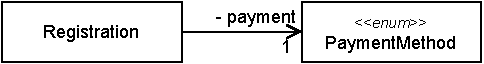
\includegraphics[width=.6\linewidth]{uml-association}
    \caption{Een registratie bevat een betalingswijze.}
    \label{fig:uml-association}
\end{figure}

We gebruiken een associatie om een algemene structurele verbinding aan te 
geven tussen twee klassen.

\subsubsection{Aggregatie (`heeft een')}
Wil je van een associatie specifiek aangeven dat het om een 
deel/geheel-relatie gaat, dan kan je de \textit{aggregatie} gebruiken.

\blockquote{
    Sometimes, you will want to model a "whole/part" relationship,
    in which one class represents a larger thing (the "whole"),
    which consists of smaller things (the "parts"). This kind of
    relationship is called aggregation, which represents a "has-a"
    relationship, meaning that an object of the whole has objects
    of the part.
}{\cite{Booch1999}, p. 67.}

Figuur~\ref{fig:uml-aggregation} laat een voorbeeld van een aggregatie zien.
Een school heeft inschrijvingen.

\begin{figure}[H]
    \centering
    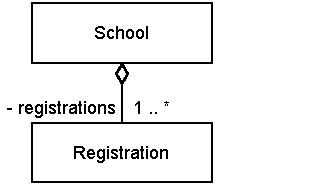
\includegraphics[height=.3\linewidth]{uml-aggregation}
    \caption{Inschrijvingen zijn onderdeel van een school, maar een school kan bestaan zonder inschrijvingen,
    bijvoorbeeld wanneer deze nog in oprichting is.}
    \label{fig:uml-aggregation}
\end{figure}

\subsubsection{Compositie (`is alleen onderdeel van')}
Wil je aangeven van de aggregatie dat het alleen onderdeel
mag zijn van deze klasse en dus niet van andere klassen,
dan geef je dat aan met een \textit{compositie}.
Dat houdt ook in dat de levensduur van de objectinstantie (deel)
gekoppeld is aan de levensduur van de objectinstantie (geheel)
waar het onderdeel van is. Over het algemeen zal een UML compositie 
dus minder snel vervangbaar zijn opgezet dan een UML aggregatie.

\blockquote{
    Composition is a form of aggregation, 
    with strong ownership and coincident lifetime
    as part of the whole. Parts with non-fixed multiplicity 
    may be created after the composite itself,
    but once created they live and die with it. 
    Such parts can also be explicitly removed before the 
    death of a composite.
    \newline\newline
    This means that, in a composite aggregation, 
    an object may be part of only one composite at a time.
    (...) This is in contrast to simple aggregation, 
    in which a part may be shared by several wholes. 
    (...) In addition, in composite aggregation (...) 
    the composite must manage the creation and destruction of its parts.
}{\cite{Booch1999}, p. 147.}

In Figuur~\ref{fig:uml-composition} is een voorbeeld van compositie te zien 
in ons voorbeeld van de schooladministratie. Volgens dit model kan een student 
niet op zichzelf bestaan, maar is altijd onderdeel van een inschrijving. 
In dit model zal het studentnummer dus gekoppeld zijn aan de inschrijving, terwijl 
in de studentklasse misschien persoonlijke informatie is opgenomen, 
zoals geboortedatum, naam, adres en woonplaats. In de praktijk zal dit op een andere
wijze gemodelleerd kunnen worden.

\begin{figure}[H]
    \centering
    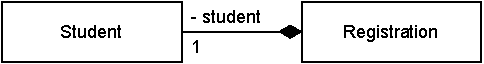
\includegraphics[width=.6\linewidth]{uml-composition}
    \caption{Een inschrijving moet altijd een student betreffen. 
    Een student kan binnen de school niet bestaan zonder inschrijving.}
    \label{fig:uml-composition}
\end{figure}

Volgens de definitie in UML is compositie dus een zeer strikte vorm 
van aggregatie. Deze definitie wordt in de praktijk echter niet zo 
strikt gehanteerd. Dit heeft te maken met het feit dat compositie 
ook een begrip is in bijvoorbeeld niet-object-georiënteerde 
talen, maar ook in wiskunde en de kunsten. In algemene zin betekent
compositie immers `samenstelling'. Dit komt meer overeen met waar 
UML de term `aggregatie' voor gebruikt.

In Figuur~\ref{fig:uml-association-aggregation-composition} zien we 
association, aggregatie en compositie in één model. Het laat zien dat je 
met een relatief eenvoudig diagram complexe ideeën kunt delen.

\begin{figure}[H]
    \centering
    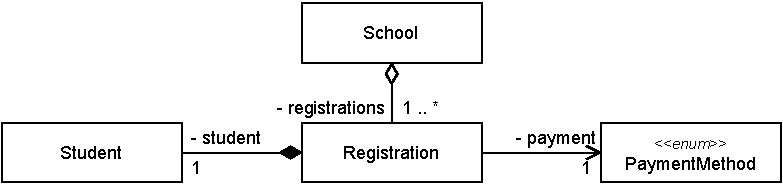
\includegraphics[width=.9\linewidth]{uml-association-aggregation-composition}
    \caption{Association, aggregatie en compositie in één model.}
    \label{fig:uml-association-aggregation-composition}
\end{figure}

\subsubsection{Overerving (`is een soort')}
Overerving (\textit{implementation inheritance}) 
geeft aan dat de subklasse (\textit{child}) een 
specifieke soort is van de superklasse (\textit{parent}) en dat er velden en methodes 
kunnen worden doorgeven van superklasse naar subklassen. 

\blockquote{
    A generalization is a relationship between a general thing (...)
    and a more specific kind of that thing.
    \newline\newline
    (...)
    \newline\newline
    Generalization means that objects of the child may be used
    anywhere the parent may appear, but not the reverse.
}{\cite{Booch1999}, p. 65.}

Binnen een school kan je denken aan verschillende soorten personeel 
\texttt{Staff}: personeel in loondienst (\texttt{SalariedStaff}) en 
personeel niet in loondienst \texttt{FreelanceStaff}, zie Figuur~\ref{fig:uml-inheritance}. 

\begin{figure}[H]
    \centering
    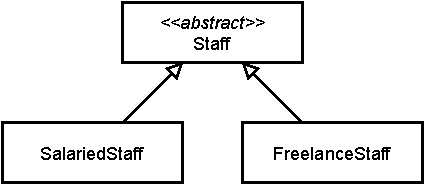
\includegraphics[height=.2\linewidth]{uml-inheritance}
    \caption{We hebben twee soorten staff: in vaste dienst of freelance.}
    \label{fig:uml-inheritance}
\end{figure}

Van \texttt{Staff} kunnen we een abstract class maken 
om bepaald gedrag te hergebruiken dat kenmerkend is voor personeel, zonder 
dat Staff op zichzelf geïnstantieerd kan worden. 
In de subklassen kunnen we dan overschrijven
wat specifiek verschilt in die klassen. Hierbij kan je bijvoorbeeld denken aan 
hoeveel er voor iemand betaald moet worden in loondienst versus als freelancer 
en hoeveel er afgedragen moet worden aan belastingen en sociale zekerheid.

\subsubsection{Realisatie (`implementeert')}
Realisatie of implementatie (\textit{interface inheritance}) geeft ook aan 
dat een subklasse een specifieke soort is van de interface, maar het is 
niet de bedoeling om zaken te overerven van het supertype. De insteek van 
een interface is om uitwisselbaarheid van implementaties te vergroten zonder 
de invulling van parent en child aan elkaar te koppelen.

\blockquote{
    A realization is a semantic relationship between classifiers
    in which one classifier specifies a contract that another
    classifier guarantees to carry out. 
}{\cite{Booch1999}, p. 149.}

Een typisch voorbeeld is de implementatie van een gateway: 
een toegangspoortje naar buiten toe, waarbij de onderliggende 
techniek kan worden uitgewisseld. Denk bijvoorbeeld aan het opslaan 
van cursussen in ons onderwijssysteem. Het feit dat we willen opslaan en uitlezen 
nemen we op in de interface. Hóe dat precies gebeurt vinden we in een implementatie.
In Figuur~\ref{fig:uml-realisation} zien we dit weergegeven: we kunnen ervoor 
kiezen om cursussen op te slaan in het bestandssysteem of in een database.

\begin{figure}[H]
    \centering
    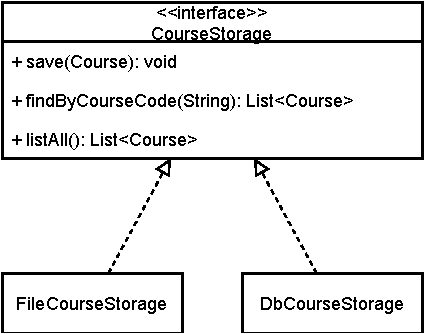
\includegraphics[height=.4\linewidth]{uml-realisation}
    \caption{De interface schrijft voor wat een CourseStorage allemaal moet kunnen. De implementaties moeten daaraan voldoende.}
    \label{fig:uml-realisation}
\end{figure}

Beide klassen zullen de methodes bevatten die worden afgedwongen door de 
interface.

\subsubsection{Subtyping, polymorfisme en dynamic binding}
De werkende principes achter overerving en realisatie zijn te vinden in 
subtyping, polymorfisme en dynamic binding.

\textit{Subtyping} houdt in dat het mogelijk is om een type-hiërarchie te hebben.
In Java is elk object bijvoorbeeld van het type Object, maar zitten er specifiekere
types onder. We kunnen subtypes definiëren door een klasse te extenden of 
een interface te implementeren. In Java kunnen klassen meerdere interfaces implementeren, 
maar slechts 1 klasse tegelijkertijd overerven. Het is wel mogelijk om het subtype verder 
steeds te extenden. Bij het verwijzen naar het type van een subklasse kan je altijd 
verwijzen naar het supertype (de interface of superklasse). Andersom is niet mogelijk.

\textit{Polymorfisme} (\textit{polymorphism}) is uit te leggen 
aan de hand van het woord zelf. Enerzijds herkennen we
het voorvoegsel \textit{poly-} (van het Griekse `πολύς', dat \textit{veel} of betekent), 
anderzijds herkennen we het woord \textit{-morfisme} (van `μορφή', dat \textit{vorm} betekent).
Polymorfisme kan men zien als `veelvormigheid': één abstractie kan verschillende vormen aannemen.
Anders gezegd: één supertype kan verschillende subtypen hebben.
Dit heeft als gevolg dat een methode, gespecificeerd in het supertype, 
in het subtype een andere vorm kan hebben. Het kan immers zijn geïmplementeerd of 
zijn overschreven.

\textit{Dynamic binding} is het mechanisme dat het in Java mogelijk maakt
een scheiding te hebben tussen de statische wereld van klassen tijdens compile time 
en de dynamische wereld van objecten tijdens runtime. Het houdt in dat
object-instanties van klassen \textit{tijdens runtime} met elkaar uitgewisseld 
worden als zij hetzelfde supertype hebben.

\blockquote{
Dynamic binding means that issuing a request doesn't commit you to a particular
implementation until run-time. Consequently, you can write programs that expect an
object with a particular interface, knowing that any object that has the correct interface
will accept the request. Moreover, dynamic binding lets you substitute objects that
have identical interfaces for each other at run-time. This substitutability is known as
\textbf{polymorphism}, and it's a key concept in object-oriented systems. It lets a client object
make few assumptions about other objects beyond supporting a particular interface.
Polymorphism simplifies the definitions of clients, decouples objects from each other,
and lets them vary their relationships to each other at run-time.
}{\cite{Gof1994}}

Subtyping, polymorfisme en dynamic binding zijn dan de sleutels 
tot flexibele object-georiënteerde software: het maakt het gemakkelijk 
om een afbakening aan te geven via interfaces of abstracte klassen 
waarvan de invulling later kan gebeuren of later vervangen kan worden.
De ene interface-implementatie kan uitgewisseld worden voor de andere,
zonder dat dat de rest van het systeem hoeft te verstoren!

\cite{Abelson1996}, paragraaf 2.4.2, noemen dit ook wel \textit{the principle of least commitment}:
subtyping, polymorfisme en dynamic binding geven ons de mogelijkheid om te koppelen tegen een (abstracte)
interface. Op die manier hoeven we ons nog niet vast te pinnen op een bepaalde implementatiekeuze!

\section{Samenvatting}
In dit hoofdstuk hebben we het object-georiënteerd modelleren en ontwerpen 
behandeld aan de hand van de belangrijkste onderdelen van het objectmodel van Booch.

\begin{defbox}{Belangrijkste elementen van het objectmodel van Booch}
    Het objectmodel van Booch onderscheid een aantal zaken
    die ons helpen goed gestructureerde object-georiënteerde software te ontwerpen:
    \begin{enumerate}
        \item \textbf{Abstraction}: klassen en objecten zijn onze kernabstracties waarin we 
        toestand (fields) en gedrag (methods) samenbrengen die bij elkaar horen. Dit verhoogt \textit{cohesion}.
        We kunnen met deze abstracties 
        communiceren via de publieke methoden. De interne werking hoeven we niet te weten (\textit{implementation hiding}).
        \item \textbf{Encapsulation}: hoe een abstractie zijn toestand bijhoudt en zijn 
        gedrag uitvoert wordt afgeschermd van de buitenwereld. Om \textit{information hiding} te bereiken wordt 
        gebruik gemaakt van access modifiers. Dit beperkt \textit{coupling}. Handige vuistregels om hierbij te helpen 
        zijn \textit{Tell, don't ask} en \textit{the Law of Demeter}.
        \item \textbf{Modularity}: klassen zijn modules waarin we toestand en gedrag samenbrengen. Daarnaast kennen 
        we interfaces om bepaald gedrag af te dwingen en enums om mogelijke waarden op te sommen. 
        Packages kunnen we gebruiken om klassen en andere modules te ordenen.
        \item \textbf{Hierarchy}: we kunnen packages onderbrengen in een logische, overzichtelijke ordening. Dat is onderdeel 
        van een softwarearchitectuur. Ook klassen en objecten kunnen in een hiërarchie tot elkaar staan. Er zijn namelijk 
        verschillende afhankelijkheden die tussen klassen kan gelden: \textit{dependency}, \textit{association}, \textit{aggregation},
        \textit{composition}, \textit{inheritance} en \textit{realisation}. Wat betreft inheritance en realisation zorgen 
        \textit{subtyping}, \textit{polymorphism} en \textit{dynamic binding} ervoor dat we een flexibele, uitwisselbare 
        invulling kunnen hebben van bepaalde abstracties. Eén abstractie kan namelijk verschillende vormen aannemen tijdens runtime:
        een subtype kan een implementatie of overschrijving verzorgen van het supertype.
    \end{enumerate}
\end{defbox}
\chapter{Softwarearchitectuur}
We willen modulaire software bereiken aan de hand van 
separation of concerns, cohesion en coupling.
Met object-oriëntatie kunnen we loose coupling en high cohesion bereiken
door een slim ontwerp te maken. 
Laten we kijken naar hoe we de gehele structuur van het project
onderhoudbaar kunnen opzetten.

Een manier om tot een onderhoudbare structuur 
te komen en deze te waarborgen is te vinden 
in \emph{softwarearchitectuur}. \index{softwarearchitectuur}
\blockquote{
    The architecture of a system constitutes what is essential 
    about that system considered in relation to its environment.
    There is no single characterization of what is essential 
    or fundamental to a system; that characterization could pertain to any or all of:
    \begin{itemize}
        \item system constituents or elements;
        \item how system elements are arranged or interrelated; 
        \item principles of the system’s organization or design; and 
        \item principles governing the evolution of the system over its life cycle.
    \end{itemize}
}{\cite{ISO42010}, p. 4}

Softwarearchitectuur draait om het maken van keuzes ten behoeve
van bepaalde kwaliteitsdoeleinden. Deze keuzes worden vormgegeven
door de functionele en non-functionele requirements en zijn vaak lastig
achteraf te wijzigen. Daarom willen we vaak van tevoren nadenken over 
verschillende technische keuzes en hoe we ons project structureren. 

We gaan later in de studie hier uitgebreid aandacht aan besteden.
Voor deze cursus hoef je dit hoofdstuk dan ook niet te kennen, maar moet je
kunnen werken binnen een modulaire, gelaagde architectuur. 
Daarvoor is het voldoende om de voorbeelden uit de opdracht te volgen. 
Mocht je echter nu al wat meer willen weten over softwarearchitectuur, 
lees dan snel verder!

\section{Modulaire architectuur}
\index{modulaire architectuur}
In een \emph{modulaire architectuur} kunnen we packages maken 
die een bepaalde rol van betekenis spelen binnen het systeem. 
Grote softwaresystemen zijn vaak ingedeeld in packages op 
verschillende niveaus die elk een andere rol vertegenwoordigen.
Een bijkomend voordeel is dat elk softwareteam tegelijkertijd 
aan een ander onderdeel kan werken.
\index{packagestructuur}
Een typische packagestructuur is als volgt. Op het hoofdniveau vertegenwoordigt
een package een \emph{component}: een losstaand onderdeel dat ziet op een subdomein van het systeem.
De packages die daaronder hangen kan je vaak beschouwen als \emph{lagen} die zien op een
bepaalde soort logica of abstractieniveau. Ten slotte kan men per laag packages opnemen 
om overzichtelijk specifieke deelgebieden aan functionaliteit te groeperen.
Dit zijn algemene \emph{subsystemen}.
In sommige softwareprojecten zijn lagen en componenten omgedraaid: 
eerst een indeling in lagen en vervolgens een indeling in losstaande componenten.

Maar wat betekenen deze rollen precies?

\subsection{Componenten}
\index{component}
Een component is een opzichzelfstaand onderdeel van een softwaresysteem
dat ziet op een bepaald deelgebied aan functionaliteit, bijvoorbeeld op een 
bepaald subdomein. Met een package diagram kan je aangeven welke 
logische componenten er zijn en hoe de relaties onderling verlopen.
Logische componenten zijn een eerste groepering van 
algemene verantwoordelijkheden op basis van functionaliteit of subdomein. 
In Figuur~\ref{fig:uml-casino-component-packages} is een package diagram opgenomen
dat de logische componenten en de relaties ertussen toont van het casinoproject.

\begin{figure}[H]
    \centering
    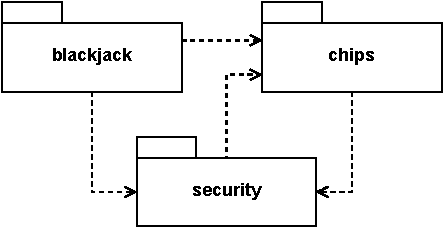
\includegraphics[width=.6\linewidth]{uml-casino-component-packages}
    \caption{Een UML-packagediagram van de logische componenten binnen het casinoproject.}
    \label{fig:uml-casino-component-packages}
\end{figure}

Vaak kun je fysieke componenten aanwijzen op basis van de herkende logische componenten.
Dit zijn componenten die niet alleen logisch samenhangen, maar ook als zodanig 
gerealiseerd (kunnen) worden. Vaak kan een fysieke component (met wat kleine aanpassingen)
aangeboden worden als zelfstandige Java-package, -module of -applicatie.
Een fysieke component biedt een manier aan om ermee te praten 
(een \emph{provided interface}, ook: \emph{componentfacade}).
Dit is een verzameling aan services, exceptions en \emph{data transfer objecten} (\emph{DTOs}) 
om met het component te praten.

Het is de bedoeling dat andere modules binnen het systeem alleen via deze 
provided interface praten met het component en niet de interne klassen rechtstreeks aanspreken.
Dit noemt men de \textit{facade convention}.
Het is een voorbeeld van \emph{implementation hiding} door middel van \emph{abstractie}.
Er is dus een soort inkapseling van klassen binnen de package van een component,
terwijl er alleen met de provided interface (de facade) gepraat wordt.

Om componenten van elkaar los te koppelen, proberen we binnen een component 
dan ook niet afhankelijk te zijn van de (interne) domeinobjecten van een andere component.
We kunnen daarvoor in de applicatie-laag met basistypen of DTOs te werken als vertalingsslag tussen 
het domein en de buitenwereld. Op die manier koppel je niet de buitenwereld aan de 
interne toestand van zo'n component. Als we naar het Chips-component kijken, 
zien we dat de componentfacade bestaat uit de ChipsService en een Balance. De ChipsService biedt 
de use cases aan van de Chips-component, terwijl de Balance een \emph{data transfer object} is 
met primitieve waarden.

De packaging binnen een component vindt plaats op basis van de functionele samenhang,
terwijl de koppeling slechts plaatsvindt tegen de klassen van de provided interface.
Dit kan bijdragen aan het bereiken van \emph{high cohesion} en \emph{loose coupling}.
De provided interface kan aangeroepen worden door een andere component,
een framework of een extern systeem. 
Zoals in Figuur~\ref{fig:uml-chips-component} is te zien,
worden de in de Chips component van het casinoproject de use case-gerichte,
taakspecifieke diensten geboden door (onder andere) de ChipsService.

Soms moet een component ook praten met andere modules of externe systemen. 
Dan biedt een component een \emph{required interface} (ookwel: \emph{componentgateway}) aan.
Dit is vaak een beschrijving van diensten die het component af wil nemen,
bijvoorbeeld van een ander component, een framework of een extern systeem.
In Figuur~\ref{fig:uml-chips-component} kunnen we zien dat de Chips component
diensten nodig heeft die zijn gedefinieerd in de ChipsRepository. Dit zullen diensten
zijn die te maken hebben met het opslaan van Chips. Dit wordt vaak ingevuld door een 
framework of library. In het casinoproject is dat een interface van Spring JPA.

\begin{figure}[H]
    \centering
    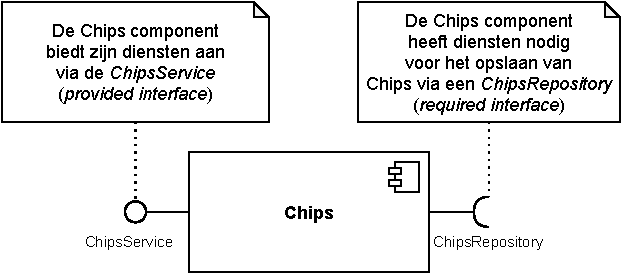
\includegraphics[width=.7\linewidth]{uml-chips-component}
    \caption{Een UML-componentdiagram van de \emph{Chips component}.}
    \label{fig:uml-chips-component}
\end{figure}

\newpage
In Java en andere object-georiënteerde talen 
zal je bij een required interface vaak een interface of abstracte klasse gebruiken.
Deze geeft aan met (abstracte) publieke methoden welke functionaliteiten vereist zijn.
Een implementerende klasse kan, door de interface te implementeren of de abstracte klasse te extenden,
aangeven dat het de benodigde functionaliteit aanbiedt in diens publieke methodes.
Het achterliggende mechanisme hiervoor is \emph{polymorfisme}.
De belofte is dat een component in zijn geheel vervangen kan worden. 
Het vervangend component moet dan wel voorzien in de vereiste functionaliteiten 
(\emph{required interface}).

\subsubsection{Wat zijn de components binnen het casinoproject?}
Hoewel we in dit project minder strikt omgaan met typische regels
voor fysieke componenten,
zou je van de structuur van het casinoproject een UML-componentdiagram kunnen maken 
zoals te zien in Figuur~\ref{fig:uml-casino-components}.
De controllers (\emph{provided interfaces}) zijn bedoeld om door Spring te 
worden aangeroepen wanneer een bepaald web request moet worden afgehandeld,
terwijl de repositories (\emph{required interfaces}) zijn bedoeld om door Spring 
te worden geïmplementeerd op basis van de benodigde opslagbehoeften.
Ook worden er application services aangeboden (\emph{provided interface})
die zowel aangeroepen worden door de controllers van de component zelf als door 
de application services van andere components.

\begin{figure}[H]
    \centering
    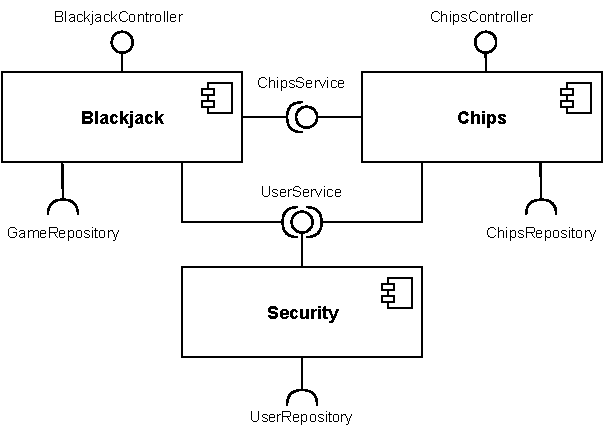
\includegraphics[width=.7\linewidth]{uml-casino-components}
    \caption{Een UML-componentdiagram van het casinoproject.}
    \label{fig:uml-casino-components}
\end{figure}

\newpage
\subsection{Lagen}
\index{gelaagde architectuur}
\index{laag}
Een applicatie, of een deel ervan, is vaak opgedeeld in lagen die 
elk verantwoordelijk zijn voor een ander soort logica binnen het systeem.
Het afhandelen van gebruikersinteractie 
is bijvoorbeeld iets heel anders dan het uitdelen van kaarten in een
kaartspel of het opslaan van een speelronde.
Een gelaagde structuur helpt niet alleen met het terugvinden van
bepaalde klassen op basis van het soort logica dat het betreft. Bij een 
losgekoppeld ontwerp kunnen lagen of onderdelen ervan gemakkelijk uitgewisseld worden.

\begin{figure}[H]
    \centering
    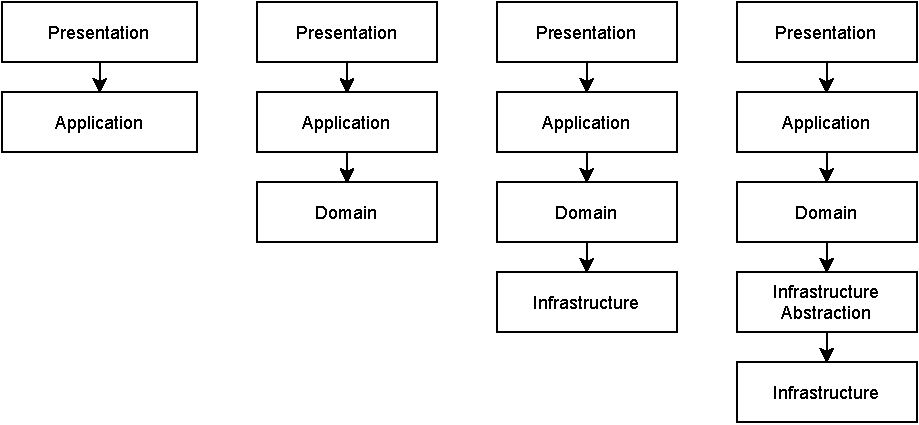
\includegraphics[width=.8\linewidth]{logical-layers}
    \caption{Voorbeelden van logische lagenmodellen met verschillende hoeveelheden lagen, waarin 
    verschillende soorten logica zitten.}
    \label{fig:logical-layers}
\end{figure}

Gelaagde architecturen komen in verschillende soorten en maten. Sommige applicaties 
zijn eerst opgesplitst in componenten en vervolgens ingedeeld in lagen. Andere zijn 
eerst opgesplitst in lagen, waarin vervolgens losse componenten zijn te bespeuren.
Het aantal lagen kan variëren tussen de twee en vijf lagen. Dit hangt af 
van de verschillende soorten logica en de specifieke architecturele eisen
van de onderdelen binnen een project. Hierbij kan je denken aan de soorten 
logica uit Tabel~\ref{table:logica-in-lagen}, gebaseerd op \cite{Pruijt2010}.

\begin{table}[H]
\centering
\begin{tabularx}{\textwidth}{|>{\raggedright}l|>{\raggedright\arraybackslash}X|}
\hline
\textbf{Logicalaag} 
    & \textbf{Verantwoordelijkheid} \\
\hline
\textit{Presentatielogica}
    & Het opbouwen en onderhouden van communicatie 
    met de gebruiker. \\ 
\hline
\textit{Taakspecifieke logica} 
    & Het coördineren van taakuitvoering en 
    het afhandelen van taakspecifieke functionaliteit. 
    In een bijbehorende laag zitten meestal applicatieservices die use cases 
    omzetten naar domeinacties met behulp van infrastructuurabstracties.
    Meestal geeft een applicatieservice een DTO terug. \\
\hline
\textit{Domeingenerieke logica}
    & Het leveren van generieke functionaliteit die te maken heeft 
    met het interessegebied van de business. 
    Domeinconcepten, business rules en entiteiten vind je vaak in lagen 
    met deze verantwoordelijkheid. \\
\hline
\textit{Infrastructuurabstractie logica}
    & Het vertalen van functionele (technologie-onafhankelijke) 
    vragen in technologieafhankelijke vragen aan de infrastructuur. 
    Hierin zitten meestal interfaces of abstracte klassen die door
    infrastructuurklassen moeten worden ingevuld (\emph{gateways}). \\
\hline
\textit{Infrastructuurlogica}
    & Het leveren van breed herbruikbare, niet businessspecifieke diensten, 
    zoals data persistentie, security, logging, deployment, etcetera. \\
\hline
\end{tabularx}
\caption{Typische soorten logica die men in aparte lagen kan aantreffen.}
\label{table:logica-in-lagen}
\index{logica in lagen}
\index{presentatielogica}
\index{taakspecifieke logica}
\index{infrastructuurabstractie logica}
\index{infrastructuurlogica}
\centering
\end{table}

\subsubsection{Regels}
Zoals er voor components geldt dat 
aanroepen naar binnen toe via de \emph{provided interface} moet gebeuren 
en aanroepen naar buiten toe via de \emph{required interface} moet gebeuren,
zo gelden er voor lagen ook vaak regels. In het geval van 
lagen zijn deze gebaseerd op het soort logica of het abstractieniveau.

Een veelvoorkomende regel is dat de afhankelijkheden enkel mogen plaatsvinden 
van hoger gelegen lagen naar lager gelegen lagen en niet andersom. 
\emph{Back calls} zijn niet toegestaan. \index{back call}
Een alternatief voor deze regel is dat afhankelijkheden enkel van buiten naar binnen
mogen lopen: van een flexibele infrastructuur (presentation en persistentie) 
naar een stabiele kern (business logic). Vaak kan je afhankelijkheden omdraaien door 
een interface of abstracte klasse tussen lagen op te nemen.

Een andere regel die je in strict layered architectures tegenkomt is dat 
afhankelijkheden geen lagen mogen overslaan. \index{strict layered architecture}
\emph{Skip calls} zijn dan niet toegestaan: \index{skip call}
tussen een hoger gelegen laag en een lager gelegen laag 
mag er alleen een afhankelijkheid zijn als er in de bedoelde
architectuur geen andere laag tussen hoort te zitten. 
Bij een drielagenarchitectuur (bijvoorbeeld: presentatie, domein, data)
mogen klassen in de presentatielaag dan niet rechtstreeks praten 
met klassen in de datalaag. Daar moet een afhankelijkheid op een
domein-module tussenzitten. Dit is vaak ook op te lossen door een tussenliggende 
interface op te nemen. De reden om dit op deze manier in te richten is om 
de koppeling tussen lagen te reduceren en het makkelijker te maken lagen (of delen daarvan)
makkelijk en flexibel inwisselbaar te maken. In relaxed layered architectures 
kom je deze regel overigens niet tegen. \index{relaxed layered architecture}

\subsubsection{Hoeveel lagen heeft het casinoproject?}
In het casinoproject is binnen components vier soorten logica te onderscheiden, 
aangewezen met packages, zie Figuur~\ref{fig:uml-casino-physical-layers}.

\begin{figure}[H]
    \centering
    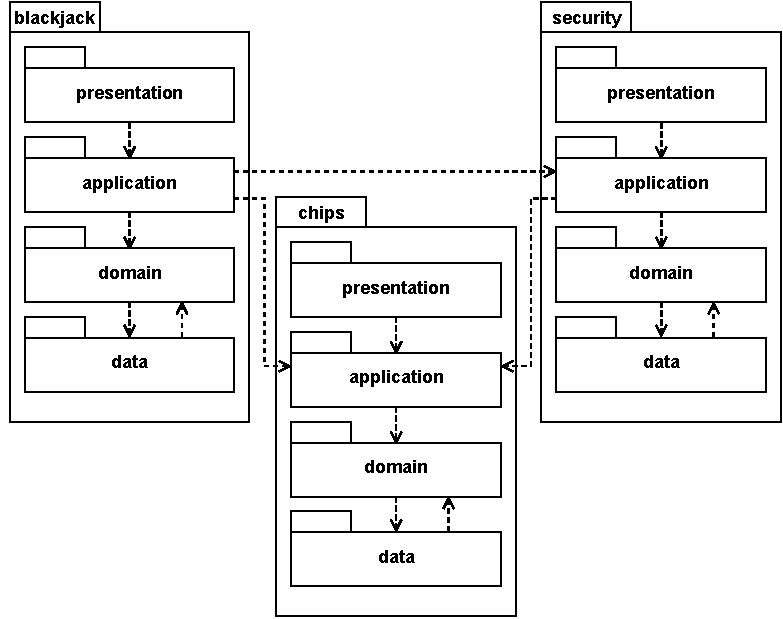
\includegraphics[width=.6\linewidth]{uml-casino-physical-layers}
    \caption{Components en layers kunnen met packages worden aangewezen binnen het casinoproject.}
    \label{fig:uml-casino-physical-layers}
\end{figure}

Deze packages corresponderen met de volgende soorten logica:
\begin{itemize}
    \item \emph{Presentation}: Presentatielogica. In het geval van een back-end API tref
    je hier alles aan dat hoort bij de technische vertaling van web requests naar Java-code. 
    Controllers (web request handlers) worden aangeroepen door het Spring framework 
    zodra een HTTP-request binnenkomt met een gedefinieerde route (HTTP-method + URL).
    \item \emph{Application}: Taakspecifieke logica. Hierin zitten applicatieservices (\emph{facades}) 
    die use cases omzetten naar domeinacties met behulp van infrastructuurabstracties. Een applicatieservices
    ziet vaak op één centraal domeinobject dat is opgebouwd uit of verwijst naar andere domeinobjecten.
    Door een applicatielaag in te richten kan dezelfde logica geboden worden onafhankelijk van de gebruikte 
    technologie in de presentatielaag: command line commando's, GUI's, web controllers of message handlers.
    \item \emph{Domain}: Domeinlogica. Domeinconcepten, business rules en entiteiten vind je vaak in lagen 
    met deze verantwoordelijkheid.
    \item \emph{Data}: Infrastructuurabstractie. Hierin zitten meestal interfaces of abstracte klassen die door
    infrastructuurklassen moeten worden ingevuld (\emph{gateways}). De daadwerkelijke infrastructuurlogica 
    wordt in het casinoproject ingevuld door het Spring framework.
\end{itemize}

Het casinoproject is dus opgezet met vier soorten logica in gedachten. Als je het 
lagenmodel echter strikt zou toepassen op Figuur~\ref{fig:uml-casino-physical-layers}, 
zie je een overtreding in de laatste twee lagen van elk component. 
De datalaag bestaat weliswaar slechts uit interfaces die door 
Spring geïmplementeerd worden, maar ze zijn afhankelijk van entities die
gedefinieerd zijn in het domein. Logisch gezien zou je het project daarom 
eerder beschouwen als een drie-lagen-architectuur. De laatste laag zou dan zowel
domeinlogica als infrastructuurabstracties bevatten. De laatste laag is opgedeeld 
in twee Java packages om de abstracte kern te scheiden van concrete 
aansluiting met infrastructuur. Het casino-project kent verder 
een relaxed layered architecture: je mag lagen overslaan.
Zo mag je in de presentatielaag een domeinobject teruggeven,
zodat het in een HTTP-response kan worden opgenomen.

\begin{figure}[H]
    \centering
    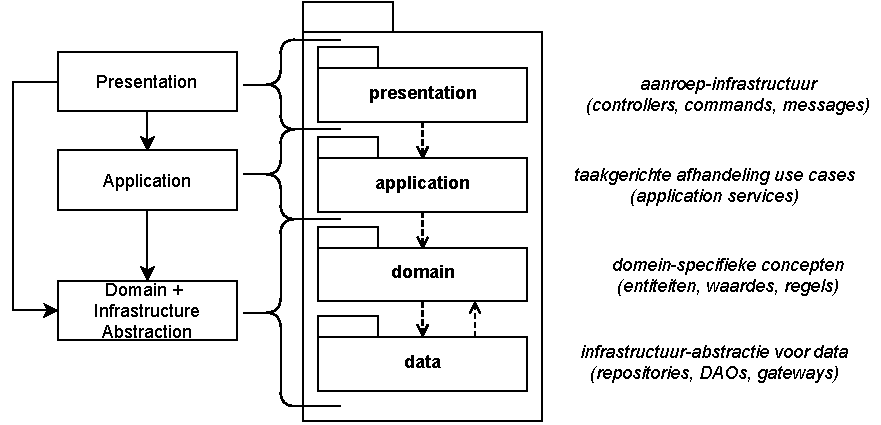
\includegraphics[width=.7\linewidth]{casino-layers}
    \caption{Het logisch en fysiek lagenmodel binnen de componenten van het casinoproject.}
    \label{fig:casino-layers}
\end{figure}

Als je het de realisatie meer wil afstemmen op de laging, zou je de 
entiteiten als losse objecten opnemen in de datalaag (als een soort DTOs) 
en een vertaalslag aanbieden tussen domeinobject en DTO. Als je daarnaast 
wil verbieden dat er lagen worden overgeslagen, zou je ook een vertaalslag 
kunnen toevoegen tussen DTO en domeinobject in de applicatielaag.
Als alternatief zou je de infrastructuur-abstractie
(de repository) kunnen opnemen in het domein en dat \textit{data} package verwijderen.
In ons project passen we deze regels echter niet zo strikt toe:
we accepteren een lichte koppeling op het framework en op ons domein.

\subsection{Subsystemen}
\index{subsysteem}
Binnen een \emph{subsysteem} kan je modules groeperen die binnen 
een laag (of component) bij elkaar horen, maar waar verder geen 
regels voor gelden. Dit is erg handig om grote projecten nog verder 
te organiseren. Je kan ervoor kiezen om subsystemen in te richten op 
basis van de technische rol die een groep modules vervuld, maar het is 
vaak mooier om ook hier aan te sluiten bij stukken samenhangende functionaliteit.
Zo kan je bijvoorbeeld binnen een domein 
(\emph{blackjack}: de logica om een blackjack spel te spelen)
een deelonderwerp aangeven 
(\emph{cards}: alles dat met kaarten te maken heeft).

\section{Packagestructuur in Java}
\index{packagestructuur}
Hiervoor hebben we het vooral over het modelleren van de conceptuele
en fysieke structuur van onze softwaremodules gehad, maar hoe kunnen we 
dit onderbrengen in onze code?

In Java kunnen we modules groeperen door gebruik te maken van 
\emph{packages} (in C\# en andere talen met \emph{namespaces}).
De naam van een Java-package lijkt op een soort omgekeerd webadres
en komt overeen met de onderliggende mappenstructuur.
Het is gebruikelijk om in Java-packages eerst te beginnen met de organisatienaam,
bijvoorbeeld \texttt{nl.hu.bep2}, en vervolgens de projectnaam \texttt{casino}.
Dan kunnen we het project opdelen in componenten, zoals in het casino-project: 
\begin{itemize}
\item \texttt{nl.hu.bep2.casino.chips}
\item \texttt{nl.hu.bep2.casino.security}
\item \texttt{nl.hu.bep2.casino.blackjack}
\end{itemize}

Binnen elke component kan wederom met packages 
onderscheid gemaakt worden naar 
het soort logica volgens een gelaagde aanpak. 
Dat leidt bij het casino-project tot de volgende 
mappen- en packagestructuur onder \texttt{src/main/java}:

\dirtree{%
    .1 nl.hu.bep2.casino.
        .2 chips.
            .3 presentation.
                .4 controller.
                .4 dto.
            .3 application.
            .3 domain.
                .4 exception.
            .3 data.
        .2 security.
            .3 presentation.
                .4 controller.
                .4 dto.
                .4 filter.
            .3 application.
            .3 domain.
            .3 data.
        .2 blackjack.
            .3 (...).
}

Als alternatief zouden we de (fysieke) componenten kunnen samenbrengen in 
modules in de zin van het Java Module System dat in Java 9 is geïntroduceerd.
Daaraan kunnen we extra regels koppelen rondom provided en required interfaces.
Daar is in het casinoproject echter niet mee gewerkt.

\section{Een voorbeeldflow}
Hoe loopt de flow binnen deze lagen? Laten we daarvoor een blik werpen 
op de \emph{deposit use case} van het Chips-component. 
Zie Figuur~\ref{fig:chips-sequence-diagram}.

\begin{figure}[H]
    \centering
    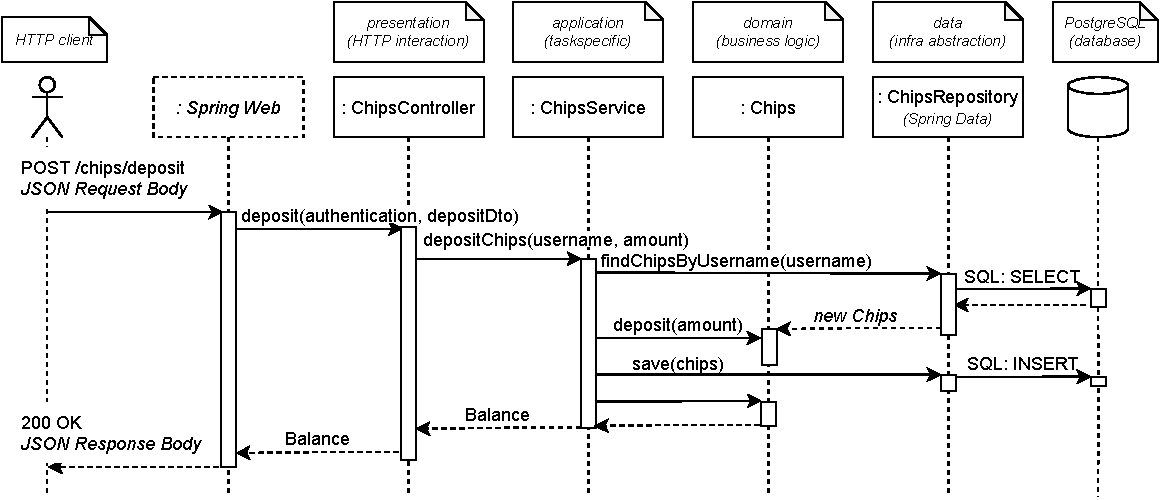
\includegraphics[width=\linewidth]{chips-sequence-diagram}
    \caption{De flow voor de deposit use case van het Chips-component}
    \label{fig:chips-sequence-diagram}
\end{figure}

Allereerst moet een HTTP-client een POST-verzoek doen naar 
\texttt{/chips/deposit}. We willen namelijk een overmaking toevoegen
aan de chips resource voor de huidige gebruiker. In dat POST-verzoek 
wordt de huidige gebruiker meegegeven via een JWT-token in de Authorization header
als deze is ingelogd. Vervolgens zet Spring Web dit verzoek om naar de bijbehorende 
controlleractie op de \emph{ChipsController} in de presentatielaag, met de
nodige informatie over de gebruiker (\emph{Authentication}) en de data die 
in de HTTP JSON Request Body zat (het \emph{Deposit} data transfer object).
De controller haalt de nodige data uit deze objecten en zet dit om naar 
een aanroep op de \emph{ChipsService} in de applicatielaag. Deze ChipsService
bevat allerlei methoden die de use cases van het Chips-component vertegenwoordigen.
De service roept de \emph{ChipsRepository} aan uit de datalaag om de hoeveelheid
\emph{Chips} op te vragen voor de betreffende \emph{User}. Vervolgens roept de 
service \emph{deposit} aan om de Chips om het aantal chips te verhogen met de 
gekozen hoeveelheid en wordt het \emph{Chips} object weer opgeslagen in de \emph{ChipsRepository}.
Ten slotte geeft de service een \emph{Balance} terug door de benodigde data uit het 
\emph{Chips}-object te halen en dit in een nieuw \emph{Balance}-object te stoppen.
De controller geeft ook deze \emph{Balance} terug aan Spring Web, waarop deze de 
\emph{Balance} omzet naar een HTTP JSON Response Body aan de hand van diens getters.

\newpage
\section{Samenvatting}
In dit hoofdstuk hebben we onderzocht op welke manier we een project kunnen 
indelen in modules ten behoeve van de onderhoudbaarheid ervan. We hebben 
kennisgemaakt met softwarearchitectuur en verschillende modulesoorten.

\begin{defbox}{Modulaire architectuur}
    Een modulaire architectuur is opgebouwd uit verschillende modules
    die elk hun eigen rol hebben binnen het gehele project.
    \newline\newline
    Fysieke \emph{componenten} zijn algemene groeperingen van deelfunctionaliteit
    die een \emph{provided interface} of \emph{componentfacade} aanbieden
    waar het component mee aangesproken kan worden. Ook kunnen ze 
    een \emph{required interface} of \emph{componentgateway} verlangen
    waarin de door het component benodigde diensten worden beschreven.
    Een component verbergt diens implementerende klassen. Daarom mag 
    er alleen via de provided interface met het component gepraat worden (\emph{facade convention}).
    \newline\newline
    Componenten kunnen worden ingedeeld in \emph{lagen} naar gelang het 
    soort logica dat daarin een rol speelt en in hoeverre een 
    onderliggende laag hergebruikt kan of moet worden. 
    Andersom kan een architect ervoor kiezen om lagen onder te verdelen in componenten.
    De aanroepen binnen een lagenmodel lopen alleen van boven naar beneden (\emph{back call ban}). 
    In een strikte laging mogen er geen lagen worden overgeslagen (\emph{skip call ban}). 
    \newline\newline
    Binnen componenten en lagen kunnen samenhangende modules in het algemeen worden
    aangegeven met \emph{subsystemen}. Dit is bijvoorbeeld handig voor het aanwijzen 
    van deelgebieden binnen een domein.
    \newline\newline
    Een onderhoudbare packagestructuur is begrijpelijk opgesteld, zodat je zaken kunt 
    terugvinden. Het helpt om aan te sluiten bij de bedoelde architecturele verdeling.
    \newline\newline
    Binnen het casinoproject is gekozen voor een indeling in componenten en lagen, 
    maar worden de regels minder streng gehanteerd. Het is bedoeld om te wennen 
    aan een modulaire opbouw. We accepteren een lichte koppeling op het framework en op ons domein.
\end{defbox}
\chapter{Libraries en frameworks}

We hebben het tot nu toe veel gehad over modules en modulariteit. 
Een groot beoogd voordeel van al deze mooie losse legoblokjes
is dat ze \emph{herbruikbaar} zijn. Maar als modulaire code herbruikbaar is, 
dan is het ook hartstikke logisch dat we modules willen (her)gebruiken die door anderen geschreven zijn.

Uiteraard doen we dit ook al, we gebruiken bijvoorbeeld de "standard library" van onze taal 
(met in Java bijvoorbeeld Math.random, of String.format), maar we hebben ook op andere vlakken andermans 
code gebruikt, om bijv. JSON te genereren. 

We worden dus afhankelijk van deze externe code om de functionaliteit van onze applicatie te implementeren. 
In vakyargon zijn we dus \emph{coupled} aan onze \emph{externe dependencies}. In principe is dit een goede zaak,
als andere mensen mooie herbruikbare code hebben geschreven scheelt ons dat mooi tijd \& moeite. Maar zoals
altijd kan je hier juist teveel, of te weinig gebruik van maken.

Het te weinig gebruik maakt van externe dependencies noemt men wel het "Not invented here"-syndroom. 
Je wantrouwt alle code die niet uit je eigen bedrijf komt. Dit heeft als grote nadeel dat je heel veel extra
code zelf zal moeten schrijven. En aangezien het niet je kerntaak is om bijv. een JSON-serializer te schrijven
zal je er veel minder tijd aan kunnen besteden, en is de kans dat de kwaliteit hieronder lijdt erg groot.

Aan de andere extreme kant is er het verhaal van \href{https://en.wikipedia.org/wiki/Npm_left-pad_incident}{Leftpad Incident}.
Leftpad was een vrij eenvoudige dependency die simpelweg spaties aan een string toevoegde. Iets dat je in relatief
korte tijd ook zelf nog wel uittypt, maar niet zo snel als dat je het als externe code van de plank kan trekken.
Je bent echter gekoppeld aan je dependencies, dus als die dependencies ineens verdwijnen, of onverwachte wijzigingen doorvoeren,
dan heb je mogelijk een groot probleem. 

Kortom we moeten altijd op zoek gaan naar de juiste balans hierin. De stabiliteit van de dependency is hierin
de belangrijkste eigenschap. Daarmee bedoelen we hoe vaak, en/of hoe groot de wijzigingen zijn die je verwacht
te moeten kunnen accepteren. Hoe stabieler de dependency, hoe minder nadelig het zal zijn om er aan gecoupled te zijn.

Nu zou je kunnen denken "Maar ik hoef toch niet te updaten? Ik kan toch gewoon de oude versie blijven gebruiken?",
en soms is dat ook zo. Echter in veel gevallen zal er vroeg of laat een kritieke bug, of beveiligingslek ontdekt 
worden, die je wel dwingt om te upgraden. Al je dependencies goed up-to-date houden is dus een goede gewoonte.

Binnen deze externe dependencies willen we wel eens onderscheid maken tussen libraries en frameworks. 
Dit is geen super-scherp onderscheid, maar het is nuttig om verschillende perspectieven te hebben. 
Het verschil zit in de 'flow of control', hoe kun je een lijn van acties door je broncode heen trekken. 

\section{Libraries}

Libraries zijn vaak wat kleinere pakketjes code, die één gericht probleem voor je oplossen. Bijvoorbeeld het 
maken van HTTP requests (Requests, Python), het genereren van JSON (Jackson, Java), het uitvullen van Strings (Leftpad, Javascript),
of het maken van complexere berekeningen zoals Annuïteiten (Finmath-lib, Java).

Het belangrijke is dat een library namens jouw code een probleem oplost of makkelijker maakt. Maar uiteindelijk is jouw applicatie nog
nog steeds \emph{de baas}.

Bij het omgaan met libraries is het belangrijk om te beslissen hoe sterk je gecoupled wil zijn aan de library.
Als je rechtstreeks vanuit jouw code een library aanroept, en je doet dat op meerdere plekken 
(stel je een Python applicatie voor die op meerdere plekken Requests gebruikt om APIs aan te roepen), dan zul je 
op al die plaatsen wijzigingen moeten doorvoeren als de library een onverwachte update uitbrengt. Dan is het een
goed idee om in plaats daarvan een eigen class te schrijven, die zelf de library aanroept, zodat je later maar
op één plek evt. dependency-problemen hoeft op te lossen.

Verder is het ook van belang om na te denken wat die library precies vertegenwoordigt. Veel libraries omvatten
de interactie met een extern systeem (zoals een database, een web-API, een barcodescanner, een webcam, etc.). Juist 
dit soort externe systemen wil je vaak extra in de gaten houden, of in (Unit-)tests kunnen vervangen door iets 
dat prettiger te testen is. Hier is het dus ook handig om een eigen class (en evt. een interface) ertussen te schuiven
zodat je flexibel blijft in hoe je applicatie met deze externe systemen omgaat.

\section{Frameworks}

Frameworks zijn ook andermans code. Maar in dit geval kiezen we ervoor om de algemene opzet en structuur van 
onze applicatie aan het framework over te laten. Denk bijvoorbeeld aan Java Servlets (BEP1, jaar 1).
Je definiëert een class, zet die op een speciale plek neer, en override de \emph{doGet} methode. En voilá je code
wordt uitgevoerd als er een HTTP-request binnen komt op een bepaald adres.

Je hebt als programmeur totaal geen zicht op de 'applicatie eromheen', alleen op jouw kleine onderdeeltje dat je er 
in hebt geschoven.

Dit is de grote kracht van frameworks, en dat zorgt er voor dat je als beginnende programmeur al direct alle soorten
applicaties ter wereld kan bouwen. Als het werkt tenminste. Als het niet werkt is het verdraaid lastig om er achter 
te komen waarom nou niet.

Het cruciale verschil met een library is dus dat het framework de baas is. De belangrijkste code in de applicatie, 
de code die jij schrijft om de requirements te implementeren, is \emph{niet} de hoofdapplicatie, maar slechts een
handig ingeschoven legoblokje dat aangeroepen wordt door het framework. Dit noemt men in vakyargon \textbf{Inversion of Control}.

\section{Spring \& Spring Boot}

Spring is een bekend Java framework uit 2004. 
In de kern is het een \textbf{Dependency Injection Container}, maar wat dat precies is komen we later op terug.

Spring is het best te zien als een soort universele kapstok voor Java code. Wat voor Java code je ook hebt
(van GUI-applicaties, Webservices en Commandline applicaties tot Database libraries en Crypto-miners) ergens in Spring
is wel een ideaal haakje om die code aan op te hangen. 

Spring Boot (2014) is een framework om je te helpen met die code ophangen. Het probleem van zo'n universele kapstok
werd namelijk (in de jaren tussen 2004 en 2014) dat het steeds ingewikkelder werd om te configureren wat nou precies
waar moest hangen, en hoe.

Spring Boot is een framework bovenop Spring die je helpt met standaard instellingen en zogeheten "Auto-configurations".
Deze Auto-configurations kun je voorstellen als dat Spring Boot automatisch bepaalde stukken code alvast voor je ophangt.
Als je bijv. ergens op een class een \emph{@RestController} annotatie plakt, dan concludeert Spring Boot automatisch dat
je kennelijk een webapplicatie wil maken (en start een webserver), en hangt die class dan op de juiste plek in die server.

Één van de meest eenvoudige zaken om mee te beginnen is een zogeheten CommandLineRunner (met @Component erop geplakt). 
Dat is het Spring equivalent van de oude \emph{public static void main}.

\subsection{Entry Point}

Ook al is het framework in principe de baas hoe de applicatie draait. Er is altijd een baas boven baas. 
We zullen helemaal aan het begin de controle aan het framework moeten geven. Met Spring Boot doen we dat zo:

\begin{listing}[H]
    \begin{minted}[linenos]{java}
    @SpringBootApplication
    public class DemoApplication {
        public static void main(String[] args){
            SpringApplication.run(DemoApplication.class, args);
        }
    }
    \end{minted}
    \caption{Minimale opstartcode voor een Spring Boot applicatie.}
    \label{code:springstart}
\end{listing}

Let er op dat deze class netjes in een (named)package zit. Spring gaat er vanuit dat 
al\footnote[]{Ok, bijna al je code, maar deze randgevallen wil je echt niet opzoeken, geloof me.} 
je code in een named package zit, en dat alle andere code in hetzelfde package, of een subpackage zit.
In iets nettere bewoording: Spring Boot doet een \emph{Component Scan} startend met het package waar 
de @SpringBootApplication class in zit en al diens subpackages.

\section{Maven}
\chapter{Services en dependency injection}

\section{Services}
\subsection{Services in Spring Boot}

\section{Dependency injection}
\subsection{Dependency injection in Spring Boot}
\chapter{Web development}

\section{HyperText Transfer Protocol (HTTP)}
\subsection{Client en server}
\subsection{Request en response}
\subsection{Requests}
\subsubsection{Methods}
\subsubsection{Responses}
\subsubsection{Statuscodes}
\subsection{Content negotiation}

\section{Representational State Transfer (REST)}
\subsubsection{Resources}
\subsubsection{Representations}
\subsubsection{Uniform Resource Locators (URLs)}
\subsubsection{HATEOAS}

\section{Webapplicaties in Spring Boot}
\subsection{Controllers (request handlers)}
\subsection{Error handling}

\subsection{Security}
\subsubsection{Authenticatie}
\subsubsection{Authorisatie}
\subsubsection{JSON Web Tokens (JWT)}

\subsection{HATEOAS met ModelAssemblers}


\chapter{Persistentie}

Een webapplicatie is standaard (/idealiter) stateless. Dat betekent dat (wat de backend betreft) elk request helemaal
uit het niets komt. Alle informatie die nodig is om dat request af te handelen moet in dat request zitten.

Als een webapplicatie echt stateless is, betekent dit dat we op elk moment de applicatie zouden moeten
kunnen herstarten, en dat we dan gewoon verder kunnen waar we gebleven waren (er was immers geen toestand
in het geheugen die door de herstart verloren is gegaan).

Dit is voor webapplicaties van belang, omdat we vaak in het echt een beetje willen kunnen sjoemelen
met het opstarten en afsluiten van applicaties. Het internet is namelijk 24/7 open, en iedereen kan 
bij elke website. Als het druk is willen we misschien alle requests over meerdere servers opsplitsen, 
en als we een update uitvoeren willen we de applicatie even afsluiten, updaten, opstarten, en dan direct weer door.

Toch willen we in onze webapplicatie met data om kunnen gaan. Een applicatie die altijd alles vergeet 
heb je niet zo gek veel aan. We willen dus dat na een herstart belangrijke data opgeslagen is geweest.
We willen dat die data blijvend (persistent) is. Meestal gebruiken we een database hiervoor. En meestal 
is dat een "relationele database", zoals bijv. PostGres.

\section{Domeinmodel versus datamodel}



% \subsection{Entity-Relationship Diagrams (ERDs)} ... geen zin in
\subsection{Object-relation impedance mismatch}

\section{Spring JPA en Hibernate}
\subsection{Entities}

\subsubsection*{Ids}

\subsection{Relaties}

\subsubsection*{Cascades}

\subsection{Repositories}

\subsection{Transacties en het belang van goed doortrekken}



\part{De opdracht}
\chapter{Opdrachtbeschrijving}

De eindopdracht van deze cursus bestaat uit een Java-project met een mondeling assessment.

HU-land Casino is een aanbieder van online kansspelen. 
Spelers kunnen met speelgeld (\textit{chips}) hun favoriete spelletjes spelen. 
Mogelijk dat HU-land Casino in de toekomst een betaalde variant op de markt wil zetten, 
maar voor nu wil het bedrijf naamsbekendheid verwerven, advertenties aanbieden en ervaring opdoen. 

Voor hun spelletjessite wil HU-land Casino een variant van het bekende \textit{blackjack} aanbieden. 
Het deel om in te loggen is overgenomen van een bestaande component (\textit{security}). 
Ook is er al enige functionaliteit om chips toe te voegen wanneer de speler deze niet meer heeft. 
Omdat nog onduidelijk is op welke technologieën wordt ingezet en met welke andere systemen gecommuniceerd zal worden, 
is het van groot belang dat deze backend onderhoudbaar en flexibel wordt opgezet. 
Het bedrijf heeft al een aantal Java-applicaties draaien met behulp van het Spring Boot framework. 
Daarom is gekozen om ook deze applicatie met Java en Spring Boot op te zetten. 
HU-land Casino heeft aangegeven waarde te hechten aan standardisatie. 
Daarom is gevraagd extra aandacht te besteden aan object oriëntatie, design principles, design patterns en REST-principes.

Er is gekozen voor een back-end applicatie om centrale controle 
te houden op het spel, terwijl met HTTP en REST compatibiliteit wordt 
geboden met verschillende front-ends, 
waaronder desktop, mobile en web apps.

Aan jou de taak om jouw ontwerp- en programmeervaardigheden in te zetten om 
een losgekoppelde, maar geïntegreerde, backend API voor het blackjackspel aan te bieden!

\newpage

\section{Het spel}
Blackjack is het bekendste kaartspel dat in casino's te vinden is.
Het spel wordt gespeeld met 1 of meer decks met 52 standaard speelkaarten.

Elke speelkaart vertegenwoordigt een bepaalde waarde gebaseerd 
op de rang (\textit{rank}) die op de kaart staat. 
De kleur (\textit{suit}) is niet van belang voor de regels 
van het spel, maar natuurlijk wel voor het weergeven van het spel.

De speler probeert de dealer te verslaan door met de score van de kaarten 
in de hand dichter bij de 21 te komen dan de dealer, 
zonder boven de 21 uit te komen.

In onze variant is er sprake van 1-speler-blackjack. Er kunnen wel 
meerdere potjes tegelijk gespeeld worden door verschillende en dezelfde 
speler. Spelers mogen niet aan elkaars spel meedoen.

\subsection{Het spelverloop}
Laten we het spelverloop van blackjack bestuderen.
Let wel\: voor een web-applicatie kan het zijn dat sommige stappen
anders kunnen verlopen, bijvoorbeeld ten behoeve van de onderhoudbaarheid
of efficiëntie. Sommige stappen worden immers volledig geautomatiseerd. 
Om dezelfde reden kunnen sommige stappen worden samengevoegd. 
Op die manier beperken we bijvoorbeeld ook de hoeveelheid netwerkcommunicatie.

Het algemene spelverloop is als volgt:
\begin{enumerate}
    \item \textit{Start game}: de speler start het spel door chips in te zetten (\textit{bet})
    \item \textit{Shuffle deck}: de dealer pakt een of meer decks van 52 speelkaarten en schudt deze 
    \item \textit{Deal cards}: de dealer deelt 1 kaart uit aan de speler, dan 1 aan zichzelf, dan 1 aan de speler en dan 1 aan zichzelf.
        \begin{itemize}
            \item De speler ziet beide kaarten in diens \textit{hand}.
            \item De speler ziet één kaart van de dealer wel (\textit{up card}) en één kaart niet (\textit{hole card}).
        \end{itemize}
    \item \textit{Check blackjack}: als de speler met twee kaarten in de hand een score heeft van precies 21
        dan eindigt het spel en:
        \begin{itemize}
            \item wint de speler $1.5\times$ diens inleg als de dealer niet ook een handscore van 21 heeft (\textit{blackjack})
            \item krijgt de speler diens inleg terug als de dealer ook een handscore van 21 heeft (gelijkspel: \textit{push})
        \end{itemize}
    \item \textit{Select move}: als het spel nog niet geëindigd is, kan de speler een move kiezen totdat deze af 
    (handscore > 21: \textit{bust}) is of het spel beëindigt
        \begin{itemize}
            \item \textit{Hit}: nog een kaart vragen; hierna volgen dezelfde opties als het de speler niet over de 21 is gegaan
            \item \textit{Stand}: met deze hand uitkomen; de dealer blijft hitten zolang zijn handwaarde onder de 17 is
            \item \textit{Double down}: de inleg verdubbelen, nog een kaart vragen en meteen uitkomen 
            \item \textit{Surrender}: opgeven en de helft van de inleg terugvragen 
        \end{itemize}
\end{enumerate}

% Het spelverloop is in kaart gebracht in Figuur~\ref{fig:conceptual-flow-blackjack}.
% Let op dat dit in onze applicatie opgebroken moet worden in use cases en dat dit 
% gevolgen heeft voor hoe onze web API eruit komt te zien.

% \begin{figure}[H]
%     \centering
%     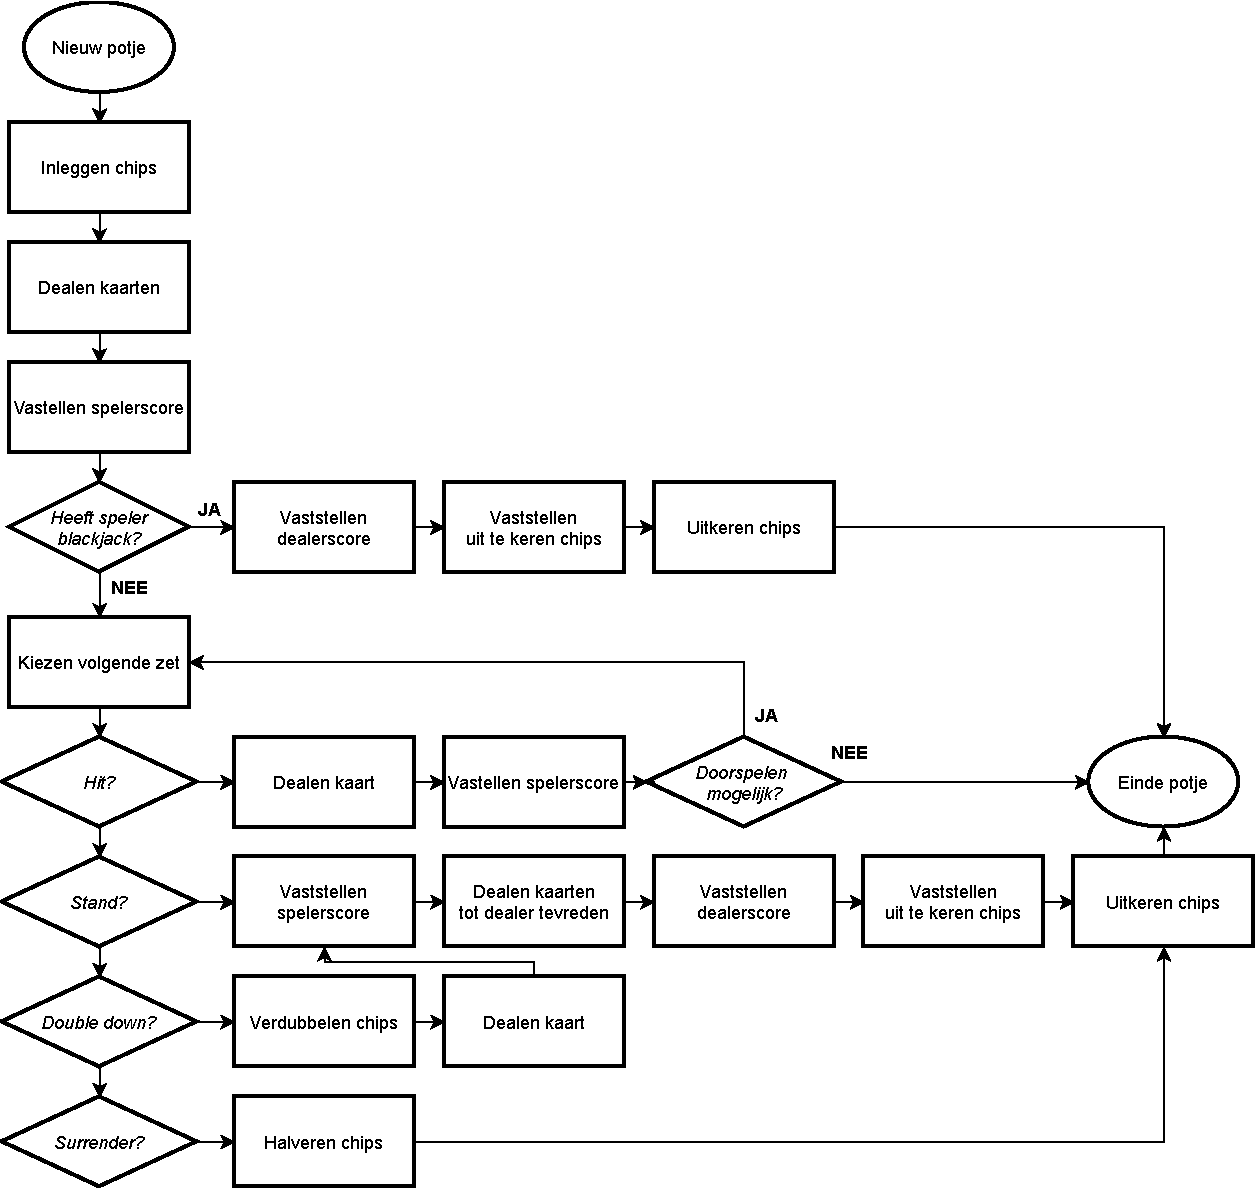
\includegraphics[width=\linewidth]{conceptual-flow-blackjack}
%     \caption{Conceptuele flowchart voor blackjack. 
%     Binnen een web-applicatie zal het er anders uitzien in verband met technische keuzes, efficiëntie en onderhoudbaarheid.}
%     \label{fig:conceptual-flow-blackjack}
% \end{figure}

\subsection{Kaart- en handscore}
Per kaart wordt de score bepaald op basis van de rang (\textit{rank}) van de kaart:

\begin{itemize}
    \item \textbf{Getallen (2 - 10)}: de waarde die erop staat
    \item \textbf{Plaatjes (Jack, Queen, King)}: de waarde 10
    \item \textbf{Aas (Ace): 1 of 11}
\end{itemize}

De handscore wordt bepaald door deze scores bij elkaar op te tellen, 
zie Tabel \ref{table:handscores}.

\begin{table}[H]
    \centering
    \begin{tabularx}{0.4\textwidth}{|l|X|}
        \hline
        \textbf{Kaarten} & \textbf{Handscore} \\ \hline
        $\heartsuit 2, \clubsuit 3$ & 5 \\ \hline
        $\clubsuit 10, \diamondsuit 5, \heartsuit 3, \spadesuit2$ & 20 \\ \hline
        $\heartsuit 10, \clubsuit K$  & 20                 \\ \hline
        $\spadesuit A, \diamondsuit 4$ & 15 (of: 5)         \\ \hline
        $\clubsuit A, \diamondsuit K$ & 21 (of: 11)         \\ \hline
        $\clubsuit A, \heartsuit A$ & 12                 \\ \hline
    \end{tabularx}
    \caption{Voorbeelden van handscores.}
    \label{table:handscores}
    \centering
\end{table}

Merk op dat de aas ertoe leidt dat de speler kan kiezen om 
met de hogere aas-score uit te komen of te hopen op betere kaarten 
met de lagere aas-score. Als de hogere aas-score boven de 21 uitkomt,
hoeven we alleen nog maar te kijken naar de lagere aas-score.

\newpage

\subsection{Speltoestanden}
Er zijn een aantal toestanden waar het spel zich in kan bevinden:
\begin{itemize}
    \item \textit{Waiting}: het spel is aangemaakt, maar nog niet gestart (optioneel)
    \item \textit{Playing}: het spel is gestart en moves kunnen worden geselecteerd
    \item \textit{Bust}: speler heeft een handscore >21 en kan niet meer verder spelen
    \item \textit{Lost}: speler heeft een lagere eindscore dan de dealer
    \item \textit{Surrendered}: speler heeft het opgegeven
    \item \textit{Push}: speler heeft dezelfde handscore als de dealer of beiden hebben een handscore van 21 in de eerste beurt
    \item \textit{Blackjack}: speler heeft een handscore van 21 in de eerste beurt en de dealer niet
    \item \textit{Won}: speler heeft een hogere handscore dan de dealer of de dealer heeft >21
\end{itemize}

\subsection{Uitbetaling}
Het uitbetalen van chips is gebaseerd op de eindtoestand (rond af naar hele chips).
Het spel eindigt alleen bij de volgende speltoestanden:

\begin{itemize}
    \item \textit{Bust}: speler krijgt niets terug
    \item \textit{Lost}: speler krijgt niets terug
    \item \textit{Surrendered}: speler krijgt $0.5\times$ zijn inleg terug
    \item \textit{Push}: speler krijgt $1\times$ zijn inleg terug
    \item \textit{Blackjack}: speler krijgt $1.5\times$ zijn inleg terug
    \item \textit{Won}: speler krijgt $2\times$ zijn inleg terug
\end{itemize}

\newpage

\section{Beoordeling}
Het gaat er bij dit vak om dat je een werkende en structureel goede back-end kan bouwen.
De snelste of kortste oplossing is voor deze cursus (en in de praktijk) niet altijd de beste oplossing!

\subsection{Assessment}
We willen ook dat je je project kunt toelichten 
aan de hand van de voor de leerdoelen relevante behandelde stof.
Dit wordt getoetst aan de hand van een project met bijbehorend interview.

Het is verstandig om je project kort te presenteren met behulp van slides.
Sta daarbij alvast stil bij de theoretische onderbouwing.

\subsubsection{Voorbeeldvragen}
Vragen die je kunt verwachten zijn gebaseerd op de leerdoelen van de cursus.
Je kan denken aan de volgende soort vragen:
\begin{itemize}
    \item Op welke manier heb je \textit{separation of concerns, loose coupling en high cohesion} bereikt?
    \item Wat houdt \textit{<object model element, design principle, design pattern>} in?
    \item Op welke manier heb je \textit{<design principle>} toegepast?
    \item Waarom zou je \textit{<object model element, design principle, design pattern, dependency injection>} gebruiken?
    \item Hoe heb je \textit{<design pattern>} in dit project uitgevoerd?
    \item Welk \textit{<design pattern>} zou je op \textit{<projectonderdeel>} kunnen toepassen?
    \item Op welke manier voldoe je aan \textit{<REST principe>}?
    \item Wat is de verantwoordelijkheid van \textit{<laag X>}?
\end{itemize}

\section{Rubric}
Zie Canvas voor de rubric van het project. Heb je alle punten gehaald, dan haal je een 10.
Mocht je wat minder scoren op bepaalde onderdelen, dan wil dat niet zeggen dat je een onvoldoende hebt!
Hier kan je natuurlijk rekening mee houden wanneer je met een planning bezig gaat.
\chapter{Opdracht 1: Projectopzet en analyse}

\section{Stap 1: Zet het project op}
Gebruik voor het project \textit{Java}, versie 11 of hoger.

Verder gebruiken we \textit{Maven}, een tool waarmee je Java-projecten kan opzetten
en gemakkelijk third-party dependencies, zoals frameworks en libraries, kunt 
gebruiken in je project. Zie hiervoor de pom.xml. Maven hoef je niet per se te 
installeren. We kunnen hiervoor onze Integrated Development Environment (IDE) gebruiken.
Ook is er een wrapper (mvnw) opgenomen in het project mocht je de commandline willen gebruiken (aanrader!). 

\subsection{Clone het project}
Clone het GitHub-project via de link die op Canvas wordt aangeboden.
We gebruik hiervoor private repositories binnen GitHub Education.
Zorg dat je een clone krijgt binnen GitHub om je werk in te leveren 
en op je machine om te werken. Open de root-directory van het project
via IntelliJ.

\subsection{Neem de opdrachtbeschrijving door}
Neem de opdrachtbeschrijving en de opdracht op Canvas door. 
Kan je (voor jezelf) antwoord geven op de volgende vragen?

\begin{enumerate}
    \item Wat moeten we precies maken?
    \item Waarom is er gekozen voor een web-applicatie?
    \item Hoe werkt blackjack ongeveer?
    \item Wat ga je ongeveer leren met deze cursus?
    \item Waar word je op beoordeeld?
    \item Waar krijg je de meeste punten voor?
    \item Wat moet je doen voor een voldoende?
\end{enumerate}

In het verleden is gebleken dat veel studenten erg laat beginnen 
en daarmee in de knoop komen met andere cursussen. Probeer dat te 
voorkomen door regelmatig je werk in te leveren, zodat je continu feedback 
kunt krijgen. Het is dus handig om voor jezelf een planning te maken.
De opdracht is om die reden opgedeeld in 6 stappen die ongeveer gelijk lopen 
met de inhoudelijke invulling van de werkcolleges.
Maak je je op enig punt tijdens de cursus zorgen over de planning,
geef het aan!

\subsection{Extra informatie: de projectstructuur}
Studenten hebben aangegeven meer informatie te willen ontvangen over hoe het 
systeem is opgezet. Daar is dit onderdeel voor bedoeld. Het is niet 
erg als je nog niet alles helemaal begrijpt of dat je niet overtuigd 
bent van deze opzet. Het gaat erom dat je in hoofdlijnen doorhebt 
waar wat te vinden is. Tijdens deze cursus gaan we er dieper op in.

Laten we eens kijken naar hoe het project is opgezet.
Onder src/main/java zien we onze packagestructuur.
Met behulp van packages kunnen we ons systeem op een logische manier 
ordenen. Dit is een belangrijke stap in het bereiken van 
\textit{separation of concerns, high cohesion en loose coupling}!

Structurele kwaliteit ziet immers op de onderhoudbaarheid
van een softwareproject. Een softwareproject heeft in algemene zin 
een goede structuur als deze is opgedeeld in kleine,
opzichzelf staande modules die intern veel samenhang 
en met elkaar beperkt koppeling vertonen.

\subsubsection{Packagestructuur in Java}
In Java kunnen we modules groeperen door gebruik te maken van 
\emph{packages} (in C\# en andere talen met \emph{namespaces}).
De naam van een Java-package lijkt op een soort omgekeerd webadres
en komt overeen met de onderliggende mappenstructuur.
Het is gebruikelijk om in Java-packages eerst te beginnen met de organisatienaam,
bijvoorbeeld \texttt{nl.hu.bep2}, en vervolgens de projectnaam \texttt{casino}.
Dan kunnen we het project opdelen in componenten, zoals in het casino-project: 
\begin{itemize}
\item \texttt{nl.hu.bep2.casino.chips}
\item \texttt{nl.hu.bep2.casino.blackjack}
\item \texttt{nl.hu.bep2.casino.security} (later)
\end{itemize}

Binnen elk component kan met packages 
onderscheid gemaakt worden naar het soort logica volgens een gelaagde aanpak. 
Dat leidt bij het casino-project tot de volgende 
mappen- en packagestructuur onder \texttt{src/main/java}:

\dirtree{%
    .1 nl.hu.bep2.casino.
        .2 chips.
            .3 application.
            .3 domain.
                .4 exception.
        .2 blackjack.
            .3 (...).
}

Het project is dus eerst opgedeeld in verschillende componenten en vervolgens in 
lagen. Voor nu is de splitsing in lagen gebaseerd op een 'application'-laag waarin 
we expliciet de verschillende usecases een plekje geven, en een 'domein'-laag waar 
we een domeinmodel realiseren (de ingrediënten van de usecases, zeg maar).

\subsection{Voorbeeld: Use cases van het chips-component}
Het chips-component biedt al een aantal use cases aan binnen ons systeem.
Deze zijn opgesomd in de ChipsService en laten zich gemakkelijk in een 
use case diagram vatten, zie: Figuur~\ref{fig:chips-use-cases}.
Kijk in de code of je dit kunt herkennen!

\begin{figure}[H]
    \centering
    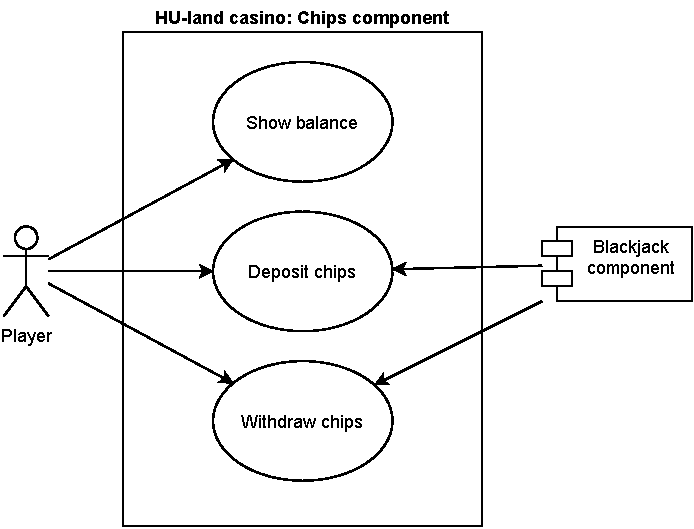
\includegraphics[height=0.4\linewidth]{chips-use-cases}
    \caption{De use cases van het chips-component}
    \label{fig:chips-use-cases}
\end{figure}

Zoals je ziet, willen we onze blackjack-component straks 
ook gebruik laten maken van de de chips-component!

\section{Stap 1: Analyseer de use cases van blackjack}
We hebben de opdracht doorgenomen en weten wat de opdrachtgever van ons verwacht.

We moeten ons voorstellen hoe blackjack precies werkt in de echte wereld.
Daarvan willen we een model maken in diagrammen en code, maar ook in ons hoofd!

Laten we een use case diagram maken, zodat de acties die door het systeem
aangeboden moeten worden voldoende duidelijk zijn. Hiervoor kan je het use case 
diagram van Figuur~\ref{fig:chips-use-cases} als inspiratie nemen.

\begin{figure}[H]
    \centering
    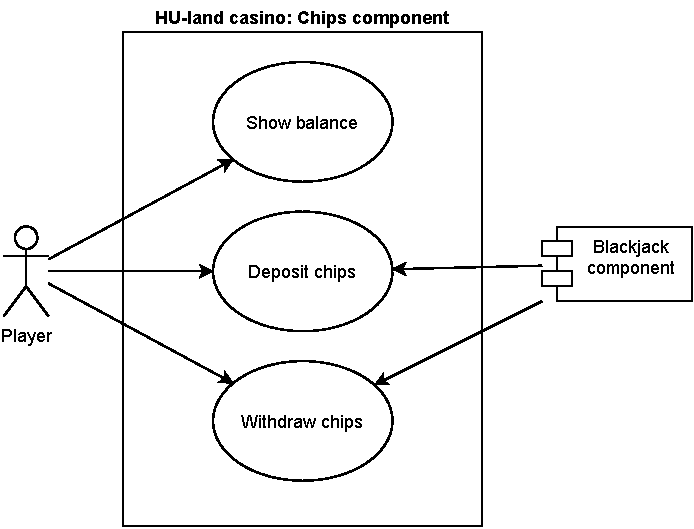
\includegraphics[height=0.4\linewidth]{chips-use-cases}
    \caption{De use cases van het chips-component}
    \label{fig:chips-use-cases}
\end{figure}

Neem de opdrachtbeschrijving door en denk na over de volgende zaken:
\begin{enumerate}
    \item Welke actors zijn er? Geautomatiseerde actors hoef je niet op te nemen.
    \item Wat wordt er binnen het component allemaal afgehandeld? Dit zijn geen use cases!
    \item Welke use cases moeten er naar buiten toe aangeboden worden om blackjack te kunnen spelen?
\end{enumerate}

Gebruik een tool als \textit{diagrams.net}, \textit{software ideas modeler} of \textit{visual paradigm},
sla het ontwerp op en exporteer het als \textit{.png} of \textit{.jpg}. 
Neem dit op in je projectdirectory (bijvoorbeeld onder een mapje \textit{diagrams}),
zodat je docent er naar kan kijken en er feedback op kan geven.

Commit je wijzigingen met een duidelijke naam, 
bijvoorbeeld: "Add use case diagram for blackjack". 
Push de wijzigingen naar je remote GitHub repository.

\section{Het objectmodel}
Wanneer je werkt met objecten, is het goed om het objectmodel van Booch in 
het achterhoofd te houden.\footnote{
    In de praktijk wordt ook wel eens verwezen naar de \textit{4 Pillars of Object Orientation}: 
    abstraction, encapsulation, polymorphism en inheritance. 
    Deze zijn in het objectmodel van Booch inbegrepen.
}

Het objectmodel van Booch onderscheidt vier belangrijke elementen 
die een rol spelen bij het object-georiënteerd modelleren:
\begin{enumerate}
    \item Abstraction
    \item Encapsulation 
    \item Modularity 
    \item Hierarchy
\end{enumerate}

Deze onderdelen noemen Booch et al. belangrijk omdat je 
zonder deze elementen geen object-georiënteerde taal (OO-taal) kan hebben.
Daarnaast beschrijven zij drie minder belangrijke elementen die je 
bij veel OO-talen tegen kunt komen: typing, persistence en concurrency.

Dit betekent natuurlijk niet dat je deze zaken buiten OO-talen niet tegen zal komen! 
Het objectmodel van Booch onderscheid een aantal zaken
die ons helpen goed gestructureerde object-georiënteerde software te ontwerpen.

Dit komt tijdens de colleges aan bod, maar kunnen we als volgt samenvatten:
\begin{enumerate}
    \item \textbf{Abstraction}: klassen en objecten zijn onze kernabstracties waarin we 
    toestand (fields) en gedrag (methods) samenbrengen die bij elkaar horen. Dit verhoogt \textit{cohesion}.
    We kunnen met deze abstracties communiceren via de publieke methoden. 
    De interne werking hoeven we dan niet te weten (\textit{implementation hiding}).
    \item \textbf{Encapsulation}: hoe een abstractie zijn toestand bijhoudt en zijn 
    gedrag uitvoert wordt afgeschermd van de buitenwereld. Om \textit{information hiding} te bereiken wordt 
    gebruik gemaakt van access modifiers (bijvoorbeeld: \textit{private}). 
    Dit beperkt \textit{coupling}. Wees spaarzaam met getters en setters (\textit{Tell, don't Ask}) 
    en wees niet afhankelijk van de onderdelen binnen een klasse \textit(\textit{Law of Demeter}).
    \item \textbf{Modularity}: klassen zijn modules waarin we toestand en gedrag samenbrengen. Daarnaast kennen 
    we interfaces om bepaald gedrag af te dwingen en enums om mogelijke waarden op te sommen. 
    Packages kunnen we gebruiken om klassen en andere modules te ordenen.
    \item \textbf{Hierarchy}: we kunnen packages onderbrengen in een logische, overzichtelijke ordening. Dat is onderdeel 
    van een softwarearchitectuur. Ook klassen en objecten kunnen in een hiërarchie tot elkaar staan. Er zijn namelijk 
    verschillende afhankelijkheden die tussen klassen kan gelden: \textit{dependency}, \textit{association}, \textit{aggregation},
    \textit{composition}, \textit{inheritance} en \textit{realisation}. Wat betreft inheritance en realisation zorgen 
    \textit{subtyping}, \textit{polymorphism} en \textit{dynamic binding} ervoor dat we een flexibele, uitwisselbare 
    invulling kunnen hebben van bepaalde abstracties. Eén abstractie kan namelijk verschillende vormen aannemen tijdens runtime:
    een subtype kan een implementatie of overschrijving verzorgen van het supertype.
\end{enumerate}

\section{Stap 2: Ontwerp een globaal domeinmodel}
Zodra je hebt nagedacht over de use cases en hier een model van hebt gemaakt,
kunnen we een overzicht maken van de concepten die we nodig hebben in ons blackjack-component.

Hiervoor kunnen we een versimpeld domeinmodel maken. 
Methods, attributes, rolnamen en multipliciteiten mag je achterwege laten.
Wees niet bang om veel concepten te modelleren!

Loop nogmaals door de opdrachtbeschrijving en verwerk de volgende zaken in je 
domeinmodel:
\begin{enumerate}
    \item Welke concepten leven er in de wereld van blackjack? 
    \item Wat zijn goede kandidaten voor klassen en enums?
    \item Wat zijn de relaties tussen deze concepten? Geef dit aan met de juiste pijlen.
    \item Welk concept kunnen we als centraal aanspreekpunt aanmerken waar we andere concepten aan kunnen hangen?
\end{enumerate}

Probeer hier niet teveel tijd aan te besteden.
Dit is een eerste opzet om het domein te structureren.
Tijdens het programmeren leren we meer over het domein, de functionaliteit en de structuur
en gaan we dit nader invullen en aanpassen!

Gebruik een tool als \textit{diagrams.net}, \textit{software ideas modeler} of \textit{visual paradigm},
sla het ontwerp op en exporteer het als \textit{.png} of \textit{.jpg}. 
Neem dit op in je projectdirectory (bijvoorbeeld onder een mapje \textit{diagrams}),
zodat je docent er naar kan kijken en er feedback op kan geven.

Commit je wijzigingen met een duidelijke naam, 
bijvoorbeeld: "Design initial domain model for blackjack". 
Push de wijzigingen naar je remote GitHub repository.

De docent geeft algemene of specifieke feedback
op basis waarvan je je domeinmodel kunt verbeteren.
Wat we alvast kunnen weggeven is dat je een spelpotje 
als centrale domeinklasse kan nemen.

\chapter{Opdracht 2: Use cases en domeinmodel}

\section{Stap 1: Analyseer de use cases van blackjack}
We hebben de opdracht doorgenomen en weten wat de opdrachtgever van ons verwacht.

We moeten ons voorstellen hoe blackjack precies werkt in de echte wereld.
Daarvan willen we een model maken in diagrammen en code, maar ook in ons hoofd!

Laten we een use case diagram maken, zodat de acties die door het systeem
aangeboden moeten worden voldoende duidelijk zijn. Hiervoor kan je het use case 
diagram van Figuur~\ref{fig:chips-use-cases} als inspiratie nemen.

\begin{figure}[H]
    \centering
    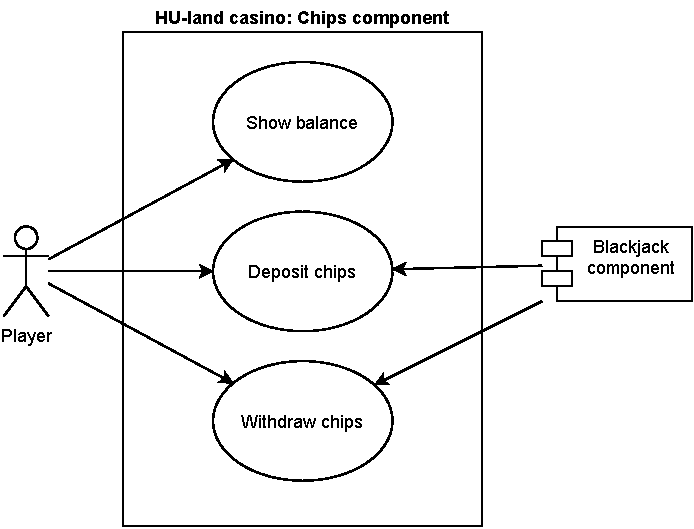
\includegraphics[height=0.4\linewidth]{chips-use-cases}
    \caption{De use cases van het chips-component}
    \label{fig:chips-use-cases}
\end{figure}

Neem de opdrachtbeschrijving door en denk na over de volgende zaken:
\begin{enumerate}
    \item Welke actors zijn er? Geautomatiseerde actors hoef je niet op te nemen.
    \item Wat wordt er binnen het component allemaal afgehandeld? Dit zijn geen use cases!
    \item Welke use cases moeten er naar buiten toe aangeboden worden om blackjack te kunnen spelen?
\end{enumerate}

Gebruik een tool als \textit{diagrams.net}, \textit{software ideas modeler} of \textit{visual paradigm},
sla het ontwerp op en exporteer het als \textit{.png} of \textit{.jpg}. 
Neem dit op in je projectdirectory (bijvoorbeeld onder een mapje \textit{diagrams}),
zodat je docent er naar kan kijken en er feedback op kan geven.

Commit je wijzigingen met een duidelijke naam, 
bijvoorbeeld: "Add use case diagram for blackjack". 
Push de wijzigingen naar je remote GitHub repository.

\section{Het objectmodel}
Wanneer je werkt met objecten, is het goed om het objectmodel van Booch in 
het achterhoofd te houden.\footnote{
    In de praktijk wordt ook wel eens verwezen naar de \textit{4 Pillars of Object Orientation}: 
    abstraction, encapsulation, polymorphism en inheritance. 
    Deze zijn in het objectmodel van Booch inbegrepen.
}

Het objectmodel van Booch onderscheidt vier belangrijke elementen 
die een rol spelen bij het object-georiënteerd modelleren:
\begin{enumerate}
    \item Abstraction
    \item Encapsulation 
    \item Modularity 
    \item Hierarchy
\end{enumerate}

Deze onderdelen noemen Booch et al. belangrijk omdat je 
zonder deze elementen geen object-georiënteerde taal (OO-taal) kan hebben.
Daarnaast beschrijven zij drie minder belangrijke elementen die je 
bij veel OO-talen tegen kunt komen: typing, persistence en concurrency.

Dit betekent natuurlijk niet dat je deze zaken buiten OO-talen niet tegen zal komen! 

\newpage
Het objectmodel van Booch onderscheid een aantal zaken
die ons helpen goed gestructureerde object-georiënteerde software te ontwerpen.

Dit komt tijdens de colleges aan bod, maar kunnen we als volgt samenvatten:
\begin{enumerate}
    \item \textbf{Abstraction}: klassen en objecten zijn onze kernabstracties waarin we 
    toestand (fields) en gedrag (methods) samenbrengen die bij elkaar horen. Dit verhoogt \textit{cohesion}.
    We kunnen met deze abstracties communiceren via de publieke methoden. 
    De interne werking hoeven we dan niet te weten (\textit{implementation hiding}).
    \item \textbf{Encapsulation}: hoe een abstractie zijn toestand bijhoudt en zijn 
    gedrag uitvoert wordt afgeschermd van de buitenwereld. Om \textit{information hiding} te bereiken wordt 
    gebruik gemaakt van access modifiers (bijvoorbeeld: \textit{private}). 
    Dit beperkt \textit{coupling}. Wees spaarzaam met getters en setters (\textit{Tell, don't Ask}) 
    en wees niet afhankelijk van de onderdelen binnen een klasse \textit(\textit{Law of Demeter}).
    \item \textbf{Modularity}: klassen zijn modules waarin we toestand en gedrag samenbrengen. Daarnaast kennen 
    we interfaces om bepaald gedrag af te dwingen en enums om mogelijke waarden op te sommen. 
    Packages kunnen we gebruiken om klassen en andere modules te ordenen.
    \item \textbf{Hierarchy}: we kunnen packages onderbrengen in een logische, overzichtelijke ordening. Dat is onderdeel 
    van een softwarearchitectuur. Ook klassen en objecten kunnen in een hiërarchie tot elkaar staan. Er zijn namelijk 
    verschillende afhankelijkheden die tussen klassen kan gelden: \textit{dependency}, \textit{association}, \textit{aggregation},
    \textit{composition}, \textit{inheritance} en \textit{realisation}. Wat betreft inheritance en realisation zorgen 
    \textit{subtyping}, \textit{polymorphism} en \textit{dynamic binding} ervoor dat we een flexibele, uitwisselbare 
    invulling kunnen hebben van bepaalde abstracties. Eén abstractie kan namelijk verschillende vormen aannemen tijdens runtime:
    een subtype kan een implementatie of overschrijving verzorgen van het supertype.
\end{enumerate}

\newpage
\section{Stap 2: Ontwerp een globaal domeinmodel}
Zodra je hebt nagedacht over de use cases en hier een model van hebt gemaakt,
kunnen we een overzicht maken van de concepten die we nodig hebben in ons blackjack-component.

Hiervoor kunnen we een versimpeld domeinmodel maken. 
Methods, attributes, rolnamen en multipliciteiten mag je achterwege laten.
Wees niet bang om veel concepten te modelleren!

Loop nogmaals door de opdrachtbeschrijving en verwerk de volgende zaken in je 
domeinmodel:
\begin{enumerate}
    \item Welke concepten leven er in de wereld van blackjack? 
    \item Wat zijn goede kandidaten voor klassen en enums?
    \item Wat zijn de relaties tussen deze concepten? Geef dit aan met de juiste pijlen.
    \item Welk concept kunnen we als centraal aanspreekpunt aanmerken waar we andere concepten aan kunnen hangen?
\end{enumerate}

Probeer hier niet teveel tijd aan te besteden.
Dit is een eerste opzet om het domein te structureren.
Tijdens het programmeren leren we meer over het domein, de functionaliteit en de structuur
en gaan we dit nader invullen en aanpassen!

Gebruik een tool als \textit{diagrams.net}, \textit{software ideas modeler} of \textit{visual paradigm},
sla het ontwerp op en exporteer het als \textit{.png} of \textit{.jpg}. 
Neem dit op in je projectdirectory (bijvoorbeeld onder een mapje \textit{diagrams}),
zodat je docent er naar kan kijken en er feedback op kan geven.

Commit je wijzigingen met een duidelijke naam, 
bijvoorbeeld: "Design initial domain model for blackjack". 
Push de wijzigingen naar je remote GitHub repository.

De docent geeft algemene of specifieke feedback
op basis waarvan je je domeinmodel kunt verbeteren.
Wat we alvast kunnen weggeven is dat je een spelpotje 
als centrale domeinklasse kan nemen.

\newpage
\section{Stap 3: Realiseer eerste domeinconcepten}
Het kan handig zijn om met deze stap te beginnen als je al wat feedback hebt 
gehad op je domeinmodel, maar je kan natuurlijk alvast beginnen en het na 
de feedback verbeteren.

We gaan de basis van ons domein leggen door alvast wat klassen aan te maken.
De methodes kunnen we nu al toevoegen, maar dit kunnen we ook later doen. 
Alvast een tip: probeer nog geen getters of setters te maken. 
Setters heb je meestal niet nodig en getters maken we pas aan wanneer
we de data daadwerkelijk uit een object moeten halen. Dit is eigenlijk alleen 
het geval wanneer je een soort vertaalslag moet uitvoeren, bijvoorbeeld tussen 
lagen of tussen ons systeem en de buitenwereld.

Laten we eerst weer de IDE induiken en beginnen met packages aan te maken!
Deze packages hebben een betekenisvolle rol in onze architectuur: 
we willen separation of concerns, high cohesion en loose coupling.

\subsection{Maak packages}
In IntelliJ kan je packages aanmaken door met de rechtermuisknop op de package
in het projectoverzicht (links) te klikken waar je iets nieuws wil toevoegen
en dan naar \texttt{New > Package} te gaan 
(je kan ook `package' typen of de pijltjestoetsen gebruiken). 
Als alternatief kan je ook de parent-package selecteren en dan 
het generate-scherm openen met \texttt{ALT + INSERT} (MacOS: \texttt{COMMAND + N}). 

Maak een nieuwe package aan: \texttt{nl.hu.bep2.casino.blackjack}.
Dit is de package voor ons component, ons deelgebied, dat over blackjack zal gaan.
We zijn bezig met het modelleren van het domein. Laten we daarvoor een laag aanmaken.
Ook daarvoor maken we een package: \texttt{nl.hu.bep2.casino.blackjack.domain}.

In deze package zouden we nog subpackages kunnen aanmaken, bijvoorbeeld om zaken te groeperen.
Denk bijvoorbeeld aan concepten die herbruikbaar zijn voor allerlei soorten kaartspellen 
in plaats van alleen voor blackjack. Dan zouden we een package kunnen aanmaken: 
\\ \texttt{nl.hu.bep2.casino.blackjack.domain.cards}. Dit kunnen we ook doen zodra we 
wat verder zijn en bekend is welke concepten er in ons domein leven.

Let op: packagenamen schrijven we in Java altijd met kleine letters,
zonder leestekens!

\subsection{Voeg klassen en enums toe}
Laten we beginnen met één centrale klasse dat ons aanspreekpunt wordt
voor domeinacties. Die klasse wordt ook het uitgangspunt wanneer we het gaan opslaan.

Maak deze centrale klasse aan. Selecteer in het projectoverzicht de 
package waaraan je een klasse wil toevoegen en klik rechtermuisknop, \texttt{New > Class}. 
Ook hier kan je hotkeys gebruiken: \texttt{ALT + INSERT} (MacOS: \texttt{COMMAND + N}).
Laten we het een Engelse naam geven dat spelpotje betekent (bijvoorbeeld: \texttt{Game} of \texttt{Table}).

Let op: klasse-, interface, en enum-namen schrijven we in Java altijd met in Pascal-case 
(\textit{StudlyCaps}), zonder leestekens!

Wat moet een spelpotje allemaal gaan bijhouden? Probeer dit op te nemen in de fields.
We willen bijvoorbeeld het huidige pakje speelkaarten bijhouden voor dit spelpotje.
Zorg dan dat je klasse er als volgt uit ziet. Vraag je af: waarom declareren we dit veld als \textit{private}?

\begin{minted}{java}
    package nl.hu.bep2.casino.blackjack.domain;

    public class Game {
        private Deck deck;
    }
\end{minted}

Als het goed is, is \texttt{Deck} in IntelliJ roodgekleurd 
of voorzien van een waarschuwing. Leer dit soort signalen te herkennen!
Om de \texttt{Deck} aan te maken, kan je met je cursor (of caret) op de het
type gaan staan (\texttt{Deck}) en de klasse laten genereren door de hotkeys
\texttt{ALT + ENTER} (MacOS: \texttt{OPTION + ENTER}) te gebruiken 
(show intention actions). Selecteer `create class' en geef de package aan 
waar je de klasse in wil aanmaken. Druk op \texttt{ENTER}.

\subsection{Vul de rest van de objectboom in}
Voeg vervolgens op deze zelfde manier alle andere velden (en de bijbehorende klassen) toe 
die deze centrale \texttt{Game}-klasse nodig heeft.
Voeg ook de velden toe van de velden van deze klasse en herhaal dit proces totdat
je je objectboom klaar hebt.

Je zou \texttt{Deck} kunnen voorzien van een verzameling van kaarten 
en een kaart weer van een rang en een kleur. Denk na over hoe je rang en kleur en 
handigst in Java kunt programmeren op een leesbare en herbruikbare manier.
Er is een manier die ervoor zorgt dat je nooit een kaart kan maken met een niet-bestaande 
rang of kleur. Er zijn maar 52 mogelijkheden: 4 kleuren en 13 rangen.

Je mag ook al methodes aanmaken, maar het gaat ons nu vooral om een eerste structuur.
We weten pas hoe de methodes precies werken zodra we onze use cases implementeren 
in een applicatie service (zie volgende opdracht).

Commit je wijzigingen met een duidelijke naam, 
bijvoorbeeld: "Structure initial domain concepts". 
Push de wijzigingen naar je remote GitHub repository.

\subsection{Maak constructors aan}
Maak voor elke klasse in ons domein een constructor aan.
Een constructor is een speciaal soort (statische) methode die wordt aangeroepen
om een objectinstantie te maken. Daar kunnen we ook instanties aan meegeven om 
de velden te vullen.

Ook constructors kan je genereren. Zet je cursor op een veld en klik 
rechtermuisknop `Show Context Actions' of gebruik de hotkey \texttt{ALT + ENTER} 
(MacOS: \texttt{OPTION + ENTER}) terwijl je caret op een veld staat. 
Je kan ook willekeurig op een plek in je klasse je caret neerzetten en iets genereren 
met \texttt{ALT + INSERT} (MacOS: \texttt{OPTION + N}).

Nu opent er een scherm om een constructor te genereren op basis van de velden. Je kan 
gemakkelijk alle velden selecteren door \texttt{SHIFT} ingedrukt te houden en 
pijltje naarbeneden te doen totdat je alle velden geselecteerd hebt. Vervolgens kan je 
op \texttt{ENTER} drukken om je keuze te bevestigen. Dan krijg je nog wat opties om de 
constructor aan te passen, maar meestal hoeft dat niet. Druk nogmaals op \texttt{ENTER}.

\begin{minted}{java}
    package nl.hu.bep2.casino.blackjack.domain.cards;

    public class Deck {
        private List<Card> cards;

        public Deck(List<Card> cards) {
            this.cards = cards;
        }
    }
\end{minted}

Je kan ook waarden initialiseren in de velden zelf. Dan hoef je ze niet mee te geven 
in de constructor, maar heeft een veld een bepaalde startwaarde wanneer een object 
geïnitialiseerd wordt. Denk bijvoorbeeld aan een lijst van kaarten, zoals in een Deck.
Als je met een lege Deck wil beginnen kan je het volgende doen:

\begin{minted}{java}
    package nl.hu.bep2.casino.blackjack.domain.cards;

    public class Deck {
        private List<Card> cards = new ArrayList<>();
    }
\end{minted}

Wil je een nieuw veld toevoegen aan een bestaande constructor? Declareer dan eerst het veld
en ga vervolgens met je caret op dit (grijze) veld staan. 
Doe wederom \texttt{ALT + ENTER} (MacOS: \texttt{OPTION + ENTER})
en kies `Add constructor parameter'.

Commit je wijzigingen met een duidelijke naam, 
bijvoorbeeld: ``Add constructors to domain concepts''. 
Push de wijzigingen naar je remote GitHub repository.

\subsection{Tip: een named constructor toevoegen aan Deck}
Beginnen met een lege Deck en van buitenaf allerlei kaarten toevoegen 
(bijvoorbeeld in de constructor of een \texttt{add(Card card)} methode)
is misschien niet de meest praktische oplossing.

Waarschijnlijk willen we elke keer als we een nieuwe Deck maken
deze vullen met kaarten. Daarvoor kunnen we een zogenaamde \textit{named constructor}
maken: een static method op \texttt{Deck} die een \texttt{Deck} teruggeeft 
na alle kaarten toegevoegd te hebben. Om een volle deck terug te geven, zouden 
we een functie met de volgende vorm kunnen aanmaken:

\begin{minted}{java}
public class Deck {
    private List<Card> cards = new ArrayList<>();

    public static Deck full() {
        Deck deck = new Deck();

        // TODO: Creation of all cards and adding them to the deck

        return deck;
    }
}
\end{minted}

Binnen de \texttt{full}-methode kunnen we kaarten toevoegen aan de 
deck-instantie door \texttt{deck.cards.add(card)} te doen. De \texttt{card}
moet je dan wel zelf aanmaken.

Hoe je precies de kaarten moet aanmaken en toevoegen aan de Deck,
laten we nog even aan jou. Afhankelijk van hoe je de kaarten gemodelleerd hebt 
in je spel, kan je dit oplossen zonder alle 52 kaarten met de hand te benoemen!

\subsection{Voeg al wat methods toe}
Het is goed om alvast wat gedrag toevoegen aan de objecten!
Maar wees niet bang om ze later aan te passen of te verwijderen.
Overbodige code is dode code.

Naast welke objecten precies welke verantwoordelijkheid hebben 
kunnen we ook nadenken over het gedrag dat zij aanbieden; 
het domein is meer dan slechts met getters en setters data heen en weer te schuiven. 
Een algemene tip is om te denken in gedrag in plaats van data. 
Setters heb je eigenlijk bijna niet nodig, getters alleen wanneer je ze aanroept. 

Probeer het object op zichzelf te beschouwen: welke vragen (queries) zou je eraan willen stellen? 
Welke acties (commands) zou je het willen laten uitvoeren? 
Waar bestaat het object uit en moet het object met andere objecten samenwerken? 
Andere objecten waarmee samengewerkt wordt, afhankelijkheden, 
kunnen we het beste in de constructor meegeven of als parameter van de methode die wordt aangeroepen. 
Het doel is om te komen tot een goed georganiseerde objectstructuur met één duidelijk aanspreekpunt: 
een game object dat later kan worden opgeslagen. 
Dit game object heeft kennis van allerlei onderliggende domeinconcepten 
die elk hun eigen specifieke verantwoordelijkheid hebben. 
Wees niet bang om veel objecten aan te maken met kleine methodes per specifieke actie! 
Ook hier komen de eigenschappen van het objectmodel om de hoek kijken.

Je kan je klassen testen door gebruik te maken van JUnit of het even 
in een Main-functie uit te proberen. We gaan het later handmatig testen met 
Postman. In een latere cursus gaan we dieper op het correct testen van object-georiënteerde projecten in.

\subsection{Tip: Gebruik je IDE!}
Wil je een klasse of package verplaatsen, versleep deze dan in het projectoverzicht.
Alle imports en verwijzingen worden automatisch geupdate. Wil je hiervoor een hotkey gebruiken,
dan is dat \texttt{F6} (MacOS: \texttt{F6}) terwijl je het betreffende item hebt geselecteerd 
in het projectoverzicht of open hebt staan in de editor. Je kan ook gebruik maken van 
het refactor-menu door rechtermuisknop op een klasse of package te doen.

Wil je een klasse of package hernoemen, dan kan je rechtermuisknop 
\texttt{Refactor > Rename} doen of de hotkeys \texttt{SHIFT + F6} (MacOS: SHIFT + F6).
Dezelfde hotkey kan je gebruiken om velden, variabelen en methoden te hernoemen.

Gebruik voor dit soort zaken altijd je IDE! Dit bespaart je een hoop tijd omdat je IDE 
het op allerlei plekken tegelijkertijd voor je aanpast. Op het hele project kan slim gebruik 
van je IDE je uren besparen! 

Er zijn nog meer van dit soort hotkeys. 
Voor een overzicht, zie: \href{https://www.jetbrains.com/help/idea/reference-keymap-win-default.html}{Windows hotkeys} 
of \href{https://www.jetbrains.com/help/idea/reference-keymap-mac-default.html}{MacOS hotkeys}.

Heb je geen zin om steeds de handleiding of Google te gebruiken? Dan kan je altijd de hotkey 
\texttt{CTRL + SHIFT + A} gebruiken om een trefwoord te typen van wat je wil doen.
Vaak geeft IntelliJ een goede suggestie. 

Wil je geïnformeerd worden wanneer je iets doet waar je een hotkey voor had kunnen gebruiken?
Dan kan je de IntelliJ-plugin Keypromotor X installeren, zie 
\href{https://www.jetbrains.com/help/idea/mastering-keyboard-shortcuts.html#learn-shortcuts}{IntelliJ's uitleg}.

\chapter{Opdracht 3: Application service}
We hebben het project aan de praat, de eisen geanalyseerd, 
de use cases gemodelleerd en de eerste domeinconcepten gerealiseerd. 
Het doet allemaal alleen nog niet zoveel!

\section{Spring Boot}
Spring Boot is een veelgebruikte standaardconfiguratie van het Spring framework. 
Vanaf gaan we ons mooie java-domein-model aanspreken met een echte Webservice.

In deze fase gebruiken we al wel de HTTP-functionaliteit van Spring (@RestControllers), maar
de database is er nog niet. Daarvoor gebruiken we een In-memory nep-implementatie. Voorlopig 
zal dus alle data ge-reset zijn elke keer dat je de applicatie opnieuw opstart (maar geen zorgen
dat pakken we later weer op!).

\subsection{Project Structuur}

Ondertussen is de mappen- en packagestructuur onder \texttt{src/main/java} een stuk uitgebreider geworden:

\dirtree{%
    .1 nl.hu.bep2.casino.
        .2 chips.
            .3 presentation.
                .4 controller.
                .4 dto.
            .3 application.
            .3 domain.
                .4 exception.
            .3 data.
        .2 security.
        .2 blackjack.
            .3 (...).
}

Het project is dus eerst opgedeeld in verschillende componenten en vervolgens in 
lagen. In lagen kunnen we zaken weer groeperen in deelsystemen. Deze componenten 
en lagen kunnen we weergeven als packages, zie Figuur~\ref{fig:uml-casino-physical-layers}.

\begin{figure}[H]
    \centering
    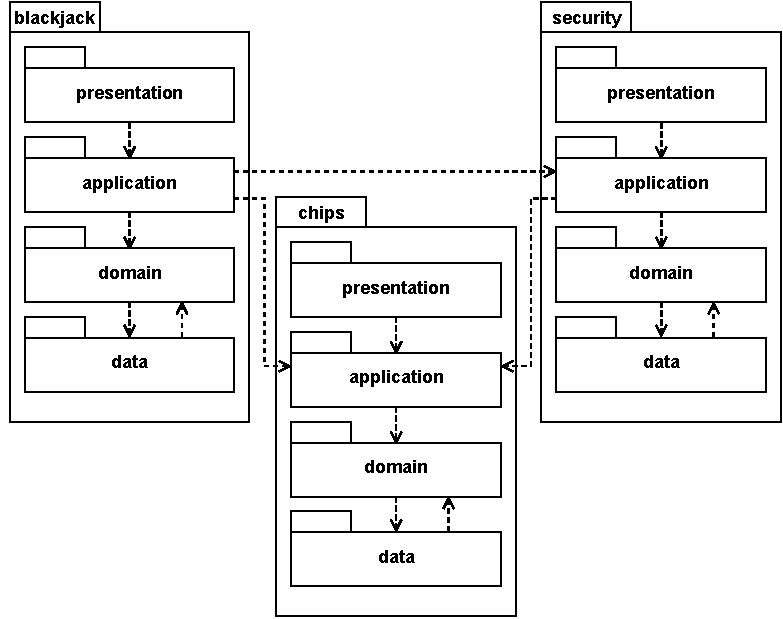
\includegraphics[width=.6\linewidth]{uml-casino-physical-layers}
    \caption{Components en layers kunnen met packages worden aangewezen binnen het casinoproject.}
    \label{fig:uml-casino-physical-layers}
\end{figure}

\subsubsection{Componenten}
Een component is een opzichzelfstaand onderdeel van een softwaresysteem
dat ziet op een bepaald deelgebied aan functionaliteit, bijvoorbeeld op een 
bepaald subdomein.

Het component bevat een aantal domeinobjecten. 
De communicatie wordt aangeboden via een service (ook: \textit{facade}). 
Deze service kan worden aangesproken door andere
services, maar ook door bijvoorbeeld een controller of een commando uit een commandline interface. 
De controller is bedoeld om HTTP-communicatie om te zetten naar Java code en vice versa. 
Andersom praat het component alleen met de buitenwereld, zoals een database, via een \textit{gateway}.

In ons project maken we gebruik van Spring om controllers te schrijven.
Deze controllers kunnen dan door Spring worden aangeroepen 
wanneer een bepaald web request moet worden afgehandeld.
Aan de andere kant maken we later ook gebruik van Spring om te voorzien in 
de data-opslag aan de hand van repositories.

\subsubsection{Lagen}
Een applicatie, of een deel ervan, is vaak opgedeeld in lagen die 
elk verantwoordelijk zijn voor een ander soort logica binnen het systeem.
Het afhandelen van gebruikersinteractie 
is bijvoorbeeld iets heel anders dan het uitdelen van kaarten in een
kaartspel of het opslaan van een speelronde.
Een gelaagde structuur helpt niet alleen met het terugvinden van
bepaalde klassen op basis van het soort logica dat het betreft. Bij een 
losgekoppeld ontwerp kunnen lagen of onderdelen ervan gemakkelijk uitgewisseld worden.

Gelaagde architecturen komen in verschillende soorten en maten. Sommige applicaties 
zijn eerst opgesplitst in componenten en vervolgens ingedeeld in lagen. Andere zijn 
eerst opgesplitst in lagen, waarin vervolgens losse componenten zijn te bespeuren.
Het aantal lagen kan variëren tussen de twee en vijf lagen. Dit hangt af 
van de verschillende soorten logica en de specifieke architecturele eisen
van de onderdelen binnen een project.

Deze packages corresponderen met de volgende soorten logica:
\begin{itemize}
    \item \emph{Presentation}: Presentatielogica. In het geval van een back-end API tref
    je hier alles aan dat hoort bij de technische vertaling van web requests naar Java-code. 
    Controllers (web request handlers) worden aangeroepen door het Spring framework 
    zodra een HTTP-request binnenkomt met een gedefinieerde route (HTTP-method + URL).
    \item \emph{Application}: Taakspecifieke logica. Hierin zitten applicatieservices (\emph{facades}) 
    die use cases omzetten naar domeinacties met behulp van infrastructuurabstracties. Een applicatieservice
    ziet vaak op één centraal domeinobject dat is opgebouwd uit of verwijst naar andere domeinobjecten.
    Door een applicatielaag in te richten kan dezelfde logica geboden worden onafhankelijk van de gebruikte 
    technologie in de presentatielaag: command line commando's, GUI's, web controllers of message handlers.
    \item \emph{Domain}: Domeinlogica. Domeinconcepten, business rules en entiteiten vind je vaak in lagen 
    met deze verantwoordelijkheid.
    \item \emph{Data}: Infrastructuurabstractie. Hierin zitten meestal interfaces of abstracte klassen die door
    infrastructuurklassen moeten worden ingevuld (\emph{gateways}).
\end{itemize}

Probeer voor jezelf de volgende vragen te beantwoorden, eventueel door naar de code te kijken.
Welke klasse is verantwoordelijk voor de vertaling van HTTP-verkeer naar Java en andersom?
In welke klassen zal je de use cases van dit component terugzien?
In welke methode wordt het aantal chips verminderd bij een afschrijving?
Hoe denk je dat de opslag geregeld is?
Stel een ander component binnen ons systeem wil Chips opnemen voor een user, welke klasse wordt dan 
eerst aangesproken?

Je mag dit met docenten en medestudenten overleggen, 
maar het antwoord op deze vragen zal naar verloop van tijd duidelijker worden.

\subsubsection*{Kanttekening: Geen écht lagenmodel}
Het casinoproject is opgezet met de verschillende soorten logica in gedachten. 
Als je het lagenmodel echter strikt zou toepassen op Figuur~\ref{fig:uml-casino-physical-layers}, 
zie je een overtreding in de laatste twee lagen van elk component. 
Hier gaan we later in dit collegejaar op in (bij de cursus \textbf{Software Architecture}),
maar misschien wil je hier al wat meer over weten.

De datalaag bestaat weliswaar slechts uit interfaces die door 
Spring geïmplementeerd worden, maar ze zijn afhankelijk van objecten (entiteiten) die
gedefinieerd zijn in het domein. Logisch gezien zou je het project daarom 
eerder beschouwen als een drie-lagen-architectuur! De laatste laag zou dan 
conceptueel zowel domeinlogica als infrastructuurabstracties bevatten. 
Deze laag is dan fysiek (in onze code) opgedeeld in twee Java packages 
om de abstracte, stabiele kern (domein) te scheiden van de meer flexibele 
aansluiting met infrastructuur via interfaces (data). 
Het casino-project kent verder een flexible layered architecture: 
je mag lagen overslaan.
Zo mag je in de presentatielaag een domeinobject teruggeven,
zodat het in een HTTP-response kan worden opgenomen, en exceptions uit het domein 
afhandelen zodat een HTTP-response de juiste statuscode kan hebben.
Dit is in veel gelaagde architecturen niet het geval. In die architecturen 
heeft een laag alleen koppeling met de laag rechtstreeks eronder.
In ons project is dit niet nodig. Het scheelt een hoop extra code en we 
tolereren de extra koppeling.

\begin{figure}[H]
    \centering
    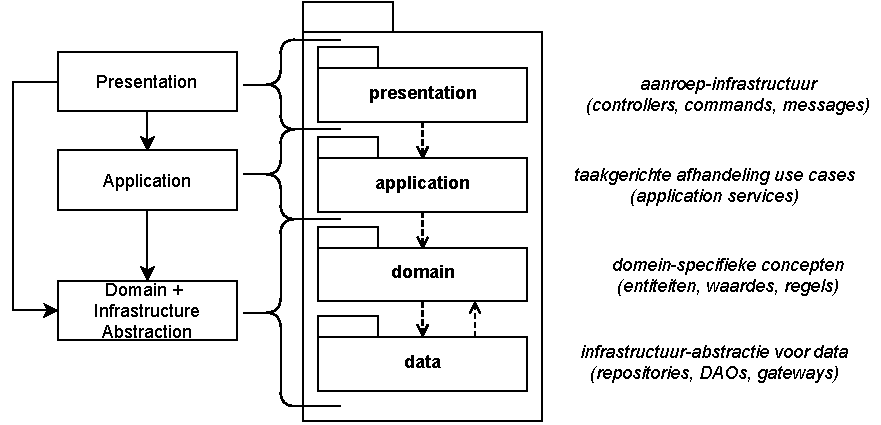
\includegraphics[width=.7\linewidth]{casino-layers}
    \caption{Het logisch en fysiek lagenmodel binnen het componenten van het casinoproject.}
    \label{fig:casino-layers}
\end{figure}

Als je de realisatie toch meer wil afstemmen op de laging, zou je de 
data-objecten en domein-objecten van elkaar splitsen en deze als losse objecten opnemen in de datalaag.
Daarvoor moet je dan daartussen een vertaalslag aanbieden. 
Als je daarnaast wil verbieden dat er lagen worden overgeslagen, 
zou je ook een vertaalslag kunnen toevoegen tussen domeinobjecten en presentatie-objecten.
Als alternatief zou je de infrastructuur-abstractie
(de repositories) kunnen opnemen in het domein en dat \textit{data} package verwijderen.
In ons project passen we deze regels echter niet zo strikt toe:
we accepteren een lichte koppeling op het framework en op ons domein.

\subsubsection{Subsystems}
Een laag kan nog verder worden opgebroken in subsystems (of \textit{deelsystemen}).
Dit zijn algemene packages die zijn bedoeld om een reeks objecten samen te verpakken.

\subsection{Voorbeeld: Structuur binnen het chips-component}
Elk component is in lagen opgedeeld. In het chips-component ziet 
dat eruit zoals in Figuur~\ref{fig:chips-layers}.

\begin{figure}[H]
    \centering
    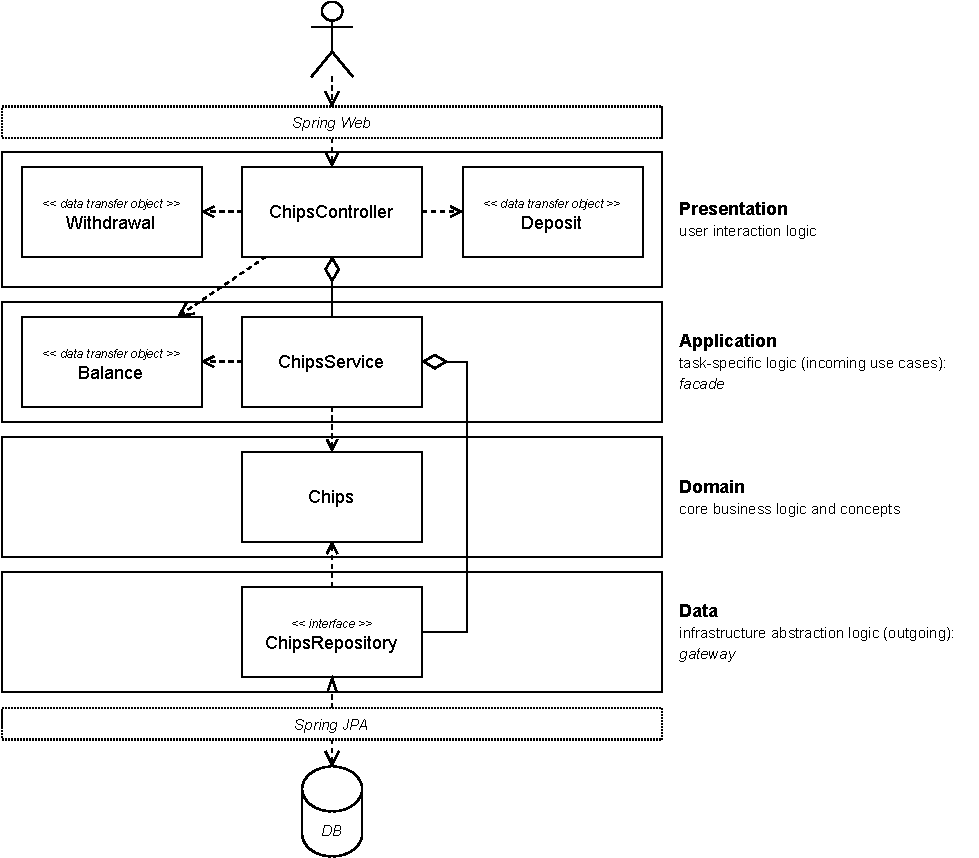
\includegraphics[width=0.8\linewidth]{chips-layers}
    \caption{De semi-gelaagde structuur binnen het chips-component.}
    \label{fig:chips-layers}
\end{figure}

\subsection{Applicatieflow}
Hoe loopt de flow binnen de de lagen in een component? 
Laten we daarvoor een blik werpen 
op de \emph{deposit use case} van het Chips-component.
Zie Figuur~\ref{fig:chips-sequence-diagram}.

\begin{figure}[H]
    \centering
    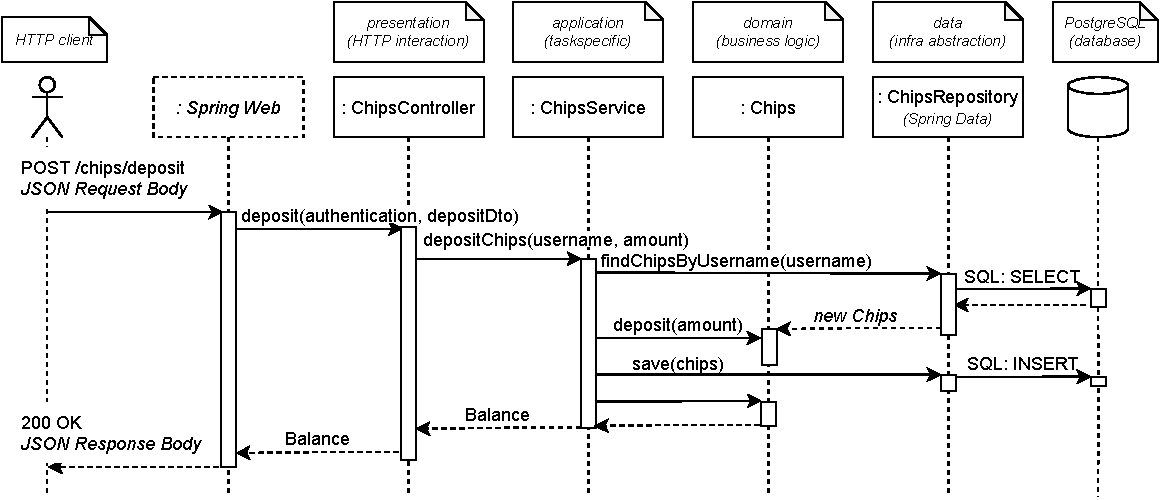
\includegraphics[width=\linewidth]{chips-sequence-diagram}
    \caption{De flow voor de deposit use case van het Chips-component}
    \label{fig:chips-sequence-diagram}
\end{figure}

Kijk ook in de code of je dit kunt herkennen!
Allereerst moet een HTTP-client een POST-verzoek doen naar 
\texttt{/chips/deposit}. We willen namelijk een overmaking toevoegen
aan de chips resource voor de huidige gebruiker. In dat POST-verzoek 
wordt de huidige gebruiker meegegeven via een JWT-token in de Authorization header
als deze is ingelogd. 

Vervolgens zet Spring Web dit verzoek om naar de bijbehorende 
controlleractie op de \emph{ChipsController} in de presentatielaag, met de
nodige informatie over de gebruiker (\emph{Authentication}) en de data die 
in de HTTP JSON Request Body zit (het \emph{Deposit} data transfer object).
De controller haalt de nodige data uit deze objecten en zet dit om naar 
een aanroep op de \emph{ChipsService} in de applicatielaag. 
Deze ChipsService bevat allerlei methoden die de use cases van 
het Chips-component vertegenwoordigen.
De service roept de \emph{ChipsRepository} aan uit de datalaag om de hoeveelheid
\emph{Chips} op te vragen voor de betreffende \emph{User} (op basis van de username). 
Vervolgens roept de service de \emph{deposit}-methode aan op de Chips om het aantal chips te verhogen met de 
gekozen hoeveelheid en wordt het \emph{Chips} object weer opgeslagen in de \emph{ChipsRepository}.
Ten slotte geeft de service een \emph{Balance} terug door de benodigde data uit het 
\emph{Chips}-object te halen en dit in een nieuw \emph{Balance}-object te stoppen.
De controller geeft ook deze \emph{Balance} terug aan Spring Web, waarop deze de 
\emph{Balance} omzet naar een HTTP JSON Response Body aan de hand van diens getters.

Voor het blackjack-component zou het ideaal zijn als wij ook één centraal object hebben 
om op te halen, domeinacties op uit te voeren en weer weg te schrijven. Het aan elkaar 
knopen daarvan kan gebeuren in use cases aangeboden in een BlackjackService!

\subsection{Frameworks}
Een \textit{framework} is code van anderen die je een hoop werk uit handen 
nemen ten aanzien van een of meer functionaliteiten. Het is een concrete, herbruikbare standaardoplossing.
Kenmerkend aan een framework is dat je als developer een deel van de controle 
uit handen geeft. Er is sprake van \textit{inversion of control}: het framework 
roept onze code aan op bepaalde plekken. Interactie met het framework vindt op twee plaatsen 
plaats:
\begin{enumerate}
    \item Entry points: hier roepen we het framework aan
    \item Hot spots: hier haken we onze eigen code in het framework en roept het framework onze code aan
\end{enumerate}

Er zijn twee soorten hot spots, die je kan herkennen vanuit het objectmodel:
\begin{enumerate}
    \item Composition hot spots: integratie van het aan een interface meegeven 
    van implementerende dependencies
    \item Inheritance hot spots: integratie via het overerven 
    van een vooropgezette klassenstructuur
\end{enumerate}

Beide vormen komen vaak voor in een framework.

In Spring herkennen we de \texttt{CasinoApplication} als entry point.
Deze is geannoteerd met \texttt{@SpringBootApplication}. Vervolgens laadt
Spring allerlei configuratie in, voert het een componentscan uit en klikt het dependencies in elkaar.
Spring's dependency injection is één van de composition hot spots die te vinden zijn in Spring,
terwijl Spring's repositories een vorm zijn inheritance hot spots.

\subsection{Dependency injection}
Dependency injection is niets anders dan het meegeven van afhankelijkheden,
in plaats van ze binnen de klasse aan te maken. Dit zorgt ervoor dat een klasse 
makkelijker uitbreidbaar en testbaar is. Hierover in een latere cursus meer.

In Spring maken we services aan door de klasse te annoteren met de \texttt{@Service} annotatie. 
We kunnen met dependency injection werken door de services (en opslagmechanismen) waarvan we afhankelijk zijn 
aan te geven in de constructor. Spring vindt dan automatisch welke services we bedoelen. 
Dit heet \textit{autowiring}.
Spring gaat tijdens een opstarten van de applicatie door onze code op zoek naar 
\texttt{@Bean}, \texttt{@Component}, \texttt{@Service}. Dit noem je Beans. 
Spring kijkt voor de dependencies naar de constructor en de benodigde interfaces 
en kijkt of er Beans zijn geconfigureerd die aan die interface voldoen. Met autowiring 
injecteert Spring de benodigde afhankelijkheid dus automatisch!

Kijk voor een voorbeeld wederom in het Chips-component.

Als alternatief voor constructor-injection kan 
je ook werken met de \texttt{@Autowired} annotatie 
op setters, constructor parameters of properties. 

Als we meerdere implementaties hebben van dezelfde interface 
(bijvoorbeeld omdat we een testimplementatie hebben), 
dan moeten we specifiek aangeven welke service we willen gebruiken. 
Dat kunnen we doen met de \texttt{@Qualifier} annotatie op zowel de service als binnen de constructor. 
Daarmee kwalificeren we om welke implementatieklasse het gaat door 
dit aan te geven boven elke \texttt{@Service} en vóór elke parameter in de 
constructor die de service gebruikt.

Met \texttt{@Value} kan je aangeven dat een waarde moet worden geïnjecteerd,
afkomstig is uit configuratie.

\section{Libraries}
Een library is ook een voorbeeld van een concrete, herbruikbare standaardoplossing.
Het belangrijkste verschil tussen een library en een framework is dat 
een framework veel meer controle opeist. Een library wordt door onze code aangeroepen
terwijl een framework uiteindelijk onze code aanroept (inversion of control).

Wel zie je vaak dat een framework gebruik maakt of zich openstelt voor verschillende
libraries door middel van composition hot spots. Vaak heb je dan een adapter nodig 
om de interface van het framework aan te passen aan de geboden facade van de library.
Dit zijn voorbeelden van design patterns. Hier gaan we het later uitgebreid over hebben.

\section{Stap 1: Maak een applicatieservice}
In ons domein hebben we een aantal domeinklassen gemaakt die verantwoordelijk 
zullen worden voor kleine acties per concept. Deze worden aan elkaar geknoopt 
door een dienstverlenend object dat verantwoordelijk is voor het omzetten van 
use cases naar domeinacties met behulp van infrastructuur. 
Dat wordt ook wel een \textit{application service} genoemd.

Maak eerst weer een package aan onder onze blackjack-component met de naam \texttt{application}
Dit is de applicatielaag waarin we onze taakgerichte logica (use cases) gaan uitvoeren.
Maak in die package een klasse aan: \texttt{BlackjackService}.
Het is immers een dienst die de acties aanbiedt om blackjack te kunnen spelen!
Deze wordt uiteindelijk aangesproken door de controller.

Vervolgens moeten we aan Spring doorgeven dat hij deze service kan gebruiken 
om te meegeven aan een andere service of bijvoorbeeld een controller als deze 
deze nodig heeft in de controller. Spring bevat een automatisch mechanisme 
voor \textit{dependency injection} en gebruikt daar annotaties voor. Om de service 
als zodanig vindbaar te maken, kan je \texttt{@Service} boven de klassedeclaratie plaatsen.

Dit zou er als volgt uit moeten zien:
\begin{minted}{java}
package nl.hu.bep2.casino.blackjack.application;

@Service
public class BlackjackService {
}
\end{minted}

\section{Stap 2: Bedenk welke methodes we nodig hebben}
Welke acties moet onze service aanbieden? 
Dit komt overeen met de use cases van onze component! 
Als het goed is, hebben we hiervoor een use case diagram gemaakt.

Maak public methods aan met de namen van deze use cases volgens 
de naming conventions van Java (\textit{camelCase}). 
Bedenk per methode ook wat voor een input we nodig hebben.
Voor sommige methoden is het handig om het spel te kunnen identificeren
op basis van een id (type: \textit{Long}). Voor de meeste methoden hebben 
we daarnaast de naam van de gebruiker nodig (type: \textit{String}).

De identifier zullen we automatisch door de database laten genereren
zodra we met persistentie bezig gaan.

\subsection{Voorbeeld: Het starten van het spel}
Laten we als voorbeeld het starten van een spel als use case nemen.
Het is belangrijk om hier een duidelijke, beschrijvende naam voor te pakken,
bijvoorbeeld: \textit{startGame} of \textit{start}.

\subsubsection{Method arguments}
Wat moeten we allemaal meegeven als parameters om het spel te starten?

Om het spel te kunnen opzoeken voor deze speler is het handig om de naam van de speler  
te bewaren. We kunnen een parameter toevoegen met als type \texttt{String} en 
als naam \texttt{playerName}. 
Omdat een speler meerdere spellen kan hebben, moeten we ervoor zorgen 
dat de database ook elk spel voorziet van een unieke identifier. 
Dat doen we later wanneer we met persistentie bezig gaan.

Het is handig om het spel meteen te beginnen met een inleg. Dat bespaart ons een
extra HTTP request! Laten we de parameter \texttt{Integer bet} toevoegen.

Meer hebben we niet nodig van de speler!

\subsubsection{Return type}
Wat willen we teruggeven nadat we het spel hebben gestart? 
Hier kunnen we wat slims verzinnen om aan de speler te laten zien hoe 
het spel er nu uitziet: de spelvoortgang. 
We willen uiteindelijk namelijk in de controller
een bericht terugsturen naar de HTTP client met daarin een JSON body 
met alle informatie. Een front-endprogrammeur kan dat mooi weergeven met
afbeeldingen en interacties.

Welke informatie willen we aan de speler laten zien
en hoe kunnen we dat het best structureren? Dat laten we aan jou over!
Alvast een tip: we kunnen een String teruggeven, 
maar dan gaat er een boel gestructureerde informatie verloren!

\subsection{Stap 3: Vul de methodes in}
Nadat we bedacht hebben welke methodes onze service moet hebben, 
kunnen we naar de invulling van die methodes kijken.
Het is het mooiste als applicatieservices niet teveel logica bevatten,
maar het gros van het werk door domeinobjecten wordt gedaan.
Op deze manier houd je een abstract en herbruikbaar domein en is je 
applicatieservice een soort samenvatting van hoe het domein zich gedraagt.

Probeer in algemene bewoordingen de acties te beschrijven 
en gaandeweg acties toe te voegen aan de centrale domeinentiteit
en de domeinobjecten die daarin gebruikt worden.

\subsubsection{Voorbeeld: Method body van startGame}
We hebben een methodenaam, parameters en een return type gedeclareerd.
Welke stappen willen we uitvoeren in de methode? 

Globaal zal je op de volgende zaken uitkomen:

\begin{enumerate}
    \item Neem het aantal chips op ter hoogte van de bet
    \item Maak een nieuw spel aan
    \item Start het spel
    \item Sla het spel op
    \item Stort chips als sprake van blackjack of push
    \item Geef de voortgang terug
\end{enumerate}

Voor het starten van het spel kan je een methode op het Game object maken,
genaamd \textit{start}. Je kan ervoor kiezen om de benodigde parameters mee te geven aan de 
constructor of de start methode. Wat deze methode moet doen laten we aan jou over.
Een aantal tips: wat moet de speltoestand zijn bij het beginnen van het spel?
Laat je het spel zelf een nieuwe Deck maken of doen we dat in de application service?

Bij de uitvoering van \textit{game.start()}, maken we onder andere gebruik van 
Deck en vast ook wel van andere klassen en enums! 
De kaarten moeten worden geschud en op de hand worden gebracht van de speler 
en van de dealer. Vervolgens moeten scores berekend worden en de huidige speltoestand 
geupdatet worden.

Het opslaan van het spel kan je nog even laten zitten,
maar het is misschien handiger om dit tijdelijk te doen 
door een field op te nemen in de application service.
Je zou hiervoor een \texttt{Map<String, Game>} kunnen gebruiken 
waarmee tijdelijk spellen (\textit{value}) bewaard kunnen worden 
op basis van spelernaam (\textit{key}).

Dit gaan we in een van de volgende opdrachten vervangen met apart object dat verantwoordelijk 
is voor de langdurige opslag van spellen: een GameRepository.

\subsubsection{Bescherm in domeinacties tegen ongeldige situaties (invariants)}
Je domein bepaalt hoe de regels van de kernconcepten eruit zien.
Bij een spel zijn het bijvoorbeeld letterlijk de spelregels.
Zie bijvoorbeeld de Chips-klasse: je mag geen negatieve hoeveelheid opnemen 
en je mag geen chips opnemen als je saldo te laag is.

\begin{minted}{java}
 public void withdraw(Long amountToWithdraw) {
    if (amountToWithdraw < 0) {
        throw new NegativeNumberException("Cannot withdraw a negative amount: " + amountToWithdraw);
    }

    long newAmount = this.amount - amountToWithdraw;
    if (newAmount < 0) {
        throw new NotEnoughChipsException(
                String.format(
                        "Cannot withdraw %d chips: %d chips remaining",
                        amountToWithdraw,
                        this.amount
                )
        );
    }

    this.amount = newAmount;
}    
\end{minted}

Voor het spelen van het spel geldt hetzelfde. Je mag natuurlijk 
geen zetten doen als het spel is afgelopen! Hiervoor kan je een \textit{guard-clause} gebruiken:
een \textit{if-statement} die een exception gooit als iets niet mag. Je hebt geen \textit{else} nodig! 
De flow wordt immers doorbroken als er sprake is van een exception.

\subsubsection{Overige use cases en domeinacties}
Doe hetzelfde voor de overige use cases en domeinacties. 
Hier gaat een boel tijd inzitten, 
dus het is niet erg als je dit later verbetert wanneer we 
de persistentie en de web API ingericht hebben.

Commit je wijzigingen met een duidelijke naam, 
bijvoorbeeld: "Add use cases to blackjack service". 
Push de wijzigingen naar je remote GitHub repository.
\documentclass[dutch,a4paper,12pt,doubleside]{book}

\usepackage[T1]{fontenc}
\usepackage[dutch]{babel}
\usepackage[utf8]{inputenc}
\usepackage[margin=3cm]{geometry}
\usepackage{amsthm}
\usepackage{hyperref}
\usepackage{minted}
\usepackage{float}
\usepackage{trimspaces}
\usepackage[nottoc]{tocbibind}
\usepackage[labelfont=bf]{caption}
\usepackage{tabularx}
\usepackage{array}
\usepackage{dirtree}

% headers and footers (page numbering)
\usepackage{fancyhdr}
\fancyhf{} % clear all header and footers
\renewcommand{\headrulewidth}{0pt} % remove the header rule
\fancyfoot[R]{\thepage} % Left side on Even pages; Right side on Odd pages
\pagestyle{fancy}
\fancypagestyle{plain}{%
  \fancyhf{}%
  \renewcommand{\headrulewidth}{0pt}%
  \fancyhf[lef,rof]{\thepage}%
}

% Card suits
\DeclareSymbolFont{extraup}{U}{zavm}{m}{n}
\DeclareMathSymbol{\varheart}{\mathalpha}{extraup}{86}
\DeclareMathSymbol{\vardiamond}{\mathalpha}{extraup}{87}

\usepackage{makeidx}
\usepackage{hyperref}
\usepackage{minted}

% New line per paragraph, instead of indentation
\usepackage[parfill]{parskip}

% Prevent balancing vertical alignment
\raggedbottom

% Sets global font
\usepackage{tgpagella}

% Font utility function
\newcommand{\fon}[1]{\fontfamily{#1}\selectfont}

\usepackage[table, x11names]{xcolor}
\definecolor{blue}{RGB}{0, 149, 200}
\definecolor{green}{RGB}{0, 200, 136}

\captionsetup{justification=raggedright,width=.8\linewidth}

\usepackage[many]{tcolorbox}
\newtcolorbox{deftbox}{
    enhanced,
    sharp corners,
    frame hidden,
    boxrule=0em,
    left=1em,
    toptitle=1em,
    top=0.25em,
    bottom=1em,
    bottomtitle=0mm,
    colback=black!4,
    colbacktitle=black!4,
    coltitle=black!60,
    fonttitle=\bfseries\small,
    fontupper=\small,
    borderline west={2pt}{0pt}{black!20},
    grow to left by=-2em,
    grow to right by=-2em
}
\newtcolorbox{defbox}[1]{
    enhanced,
    sharp corners,
    frame hidden,
    boxrule=0em,
    left=1em,
    toptitle=1em,
    top=0.25em,
    bottom=1em,
    bottomtitle=0mm,
    colback=black!4,
    colbacktitle=black!4,
    coltitle=black!60,
    fonttitle=\bfseries\small,
    fontupper=\small,
    borderline west={2pt}{0pt}{black!20},
    grow to left by=-2em,
    grow to right by=-2em,
    title={#1}
}
\newtcolorbox{quotebox}{
    enhanced,
    sharp corners,
    frame hidden,
    left=1em,
    right=1em,
    top=1em,
    bottom=1em,
    colback=black!4!white,
    fontupper=\small,
    grow to left by=-2em,
    grow to right by=-2em
}

\def\trim#1{\ignorespaces#1\unskip}

\newcommand{\blockquote}[2]{
    \hfill
    \begin{quotebox}
    \begin{flushleft}
        ``\trim{#1}''
        \newline\newline\rightline{\textbf{-- \trim{#2}}}
    \end{flushleft}
    \end{quotebox}
    \noindent
}

\renewcommand{\listingscaption}{Codevoorbeeld}
\renewcommand{\listoflistingscaption}{Overzicht van codevoorbeelden}
\counterwithin{listing}{chapter}
% \usepackage[chapter]{minted}



\begin{document}

\setcounter{chapter}{3}
\chapter{Opdracht 4: Web API}
Onze applicatie presenteert zichzelf naar buiten toe via het web:
we reageren op HTTP requests en geven HTTP responses terug.

\section{Client/server-architectuur}
Het web werkt volgens een client/server-architectuur (of klant/bediende-model):
We hebben een client, bijvoorbeeld een web browser, die een verzoek doet 
aan een server die dit afhandelt. Zie Figuur~\ref{fig:client-server}.

\begin{figure}[H]
    \centering
    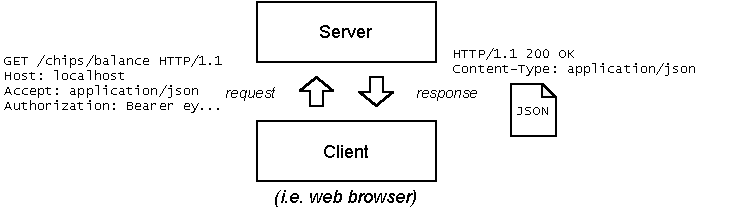
\includegraphics[width=.9\linewidth]{client-server}
    \caption{HTTP requests worden van een client gestuurd naar een server, welke dit verwerkt en reageert met een HTTP response.}
    \label{fig:client-server}
\end{figure}

\section{Content negotiation}
Zoals in Figuur~\ref{fig:client-server} is te zien, 
onderhandelen client en server over het ophalen van een \textit{representatie}
van een bepaalde \textit{resource}. We zien dat de client een 
GET-verzoek doet naar localhost voor een Balance-resource te
vinden via de Uniform Resource Locator (URL) `chips/balance'
(in combinatie met de token in de Authorization header)
De gewenste representatie daarvan moet `application/json' zijn.

Deze interactie tussen client en server noem je \texit{content negotation}:
er is een scheiding tussen de abstractie en de verschijningsvorm ervan.

\section{HTTP requests}
Een HTTP request (zie Figuur~\ref{fig:client-server}) wordt gevormd door:
\begin{enumerate}
    \item Een beschrijving van method, URI en protocol
    \item Headers
    \item Optioneel: een request body met een representatie volgens Content-Type
\end{enumerate}

\subsection{HTTP methods}
De HTTP-specificatie beschrijft een aantal methodes 
waarmee een client allerlei zaken kan vragen aan een server.
Het is belangrijk om de juiste HTTP-methodes te gebruiken omdat 
deze in de eerste plaats het soort actie aangeven die wordt verzocht.

In de tweede plaats staat in de protocol-specificatie van HTTP heel 
nauwkeurig beschreven wat clients en servers mogen verwachten van een 
bepaalde HTTP-methodes. 
Twee van de te verwachten eigenschappen zijn \textit{safety}
en \textit{idempotentie}.

Een HTTP-method wordt als \textit{safe} beschouwt als deze niet 
de intentie heeft om de servertoestand aan te passen. 
Dat betekent dat het gaat om read-only methoden. Safe 
methoden kunnen helpen bij het cachen van resultaten (zie: REST).
Bij safety gaat het dus niet om de beveiliging, het ziet 
erop dat het veilig is omdat het geen toestand kan aanpassen.

Wanneer een HTTP-method \textit{idempotent} wordt genoemd,
betekent dat dat we het verzoek meerdere keren kunnen herhalen
zonder dat de uitkomst op server verandert. Denk bijvoorbeeld aan 
het tweemaal uitvoeren van een \texttt{DELETE}-methode. Beide keren is 
de betreffende resource verwijderd. Idempotentie helpt een API betrouwbaar 
te maken tegen fouten: het betekent dat je een verzoek kan herhalen zonder 
als je als client niet zeker weet of het is aangekomen of niet.

We kennen de volgende HTTP-methods, zie Figuur~\ref{table:http-methods}:

\begin{table}[H]
\centering
\begin{tabularx}{\textwidth}{
    |>{\raggedright}l|>{\raggedright}X|>{\raggedright}X|>{\raggedright\arraybackslash}X|
}
\hline
\textbf{Method} & \textbf{Bedoeling} & \textbf{Safe} & \textbf{Idempotent} \\ \hline
\texttt{GET} & opvragen van resource(s) & Ja & Ja \\ \hline
\texttt{HEAD} & opvragen van headers (voordat je een mogelijk grote GET-request doet) & Ja & Ja \\ \hline
\texttt{OPTIONS} & opvragen van toegestane communicatiewijzen voor een bepaalde URL of server & Ja & Ja \\ \hline
\texttt{TRACE} & opvragen van afgelegde weg van het verzoek ter debugging & Ja & Ja \\ \hline
\texttt{DELETE} & verwijderen van gehele resource op basis van URL (met identifier) & Nee & Ja \\ \hline
\texttt{PUT} & aanmaken/wijzigen van gehele resource op basis van URL (met identifier) & Nee & Ja \\ \hline
\texttt{PATCH} & wijzigen van deel van resource op basis van URL (met identifier) & Nee & Nee \\ \hline
\texttt{POST} & aanmaken nieuwe resource op onder een bepaalde URL (zonder identifier) & Nee & Nee \\ \hline
\end{tabularx}
\caption{Een opsomming van HTTP-methoden, hun bedoeling en verwachte eigenschappen}
\label{table:http-methods}
\centering
\end{table}

\newpage
\section{HTTP responses}
Een HTTP response (zie Figuur~\ref{fig:client-server}) wordt gevormd door:
\begin{enumerate}
    \item Een beschrijving van protocol en statuscode
    \item Headers
    \item Optioneel: response body met een representatie volgens Content-Type 
\end{enumerate}

\subsection{Status codes}
Het teruggeven van de juiste statuscode is erg belangrijk wanneer je een API 
ontwerpt. Het maakt een bepaalde verwachting duidelijk en clients krijgen zo 
de mogelijkheid om slim om te gaan als er bijvoorbeeld een redirection moet plaatsvinden
of als de client wat verkeerd heeft gedaan.

HTTP status codes worden onderverdeeld 5 categorieën, waarbij 
het eerste getal steeds de categorie aangeeft (we noemen er hier een paar):
\begin{itemize}
    \item \textbf{1xx Informational}: request ontvangen, verwerking gaat door
        \begin{itemize}
            \item \textbf{100 Continue}: wordt gebruikt als een client eerst wil checken of de server het verzoek 
            gaat accepteren, bijvoorbeeld bij grote request bodies.
        \end{itemize}
    \item \textbf{2xx Successful}: request ontvangen, begrepen, en geaccepteerd zonder problemen
        \begin{itemize}
            \item \textbf{200 OK}: standaardresponse voor succesvolle afhandeling
            \item \textbf{201 Created}: verzoek is afgehandeld; een resource is succesvol aangemaakt
            \item \textbf{202 Accepted}: verzoek is succesvol binnengekomen, maar de uitvoering volgt nog
        \end{itemize}
    \item \textbf{3xx Redirection}: meer actie is vereist om het verzoek af te handelen
    \begin{itemize}
        \item \textbf{303 See Other}: de response voor het request kan worden opgehaald (met GET) via de getoonde URI
        \item \textbf{307 Temporary Redirect}: dit verzoek, niet volgende verzoeken, moet worden herhaald naar een andere URI (met dezelfde method)
        \item \textbf{308 Permanent Redirect}: dit verzoek en volgende verzoeken moeten worden herhaald naar een andere URI (met dezelfde method)
    \end{itemize}
    \item \textbf{4xx Client Error}: de client heeft iets fout gedaan bij het doen van het verzoek
    \begin{itemize}
        \item \textbf{400 Bad Request}: algemene fout om aan te geven dat het request van de client niet klopt
        \item \textbf{401 Unauthorized}: lijkt op 403, maar client moet zich authenticeren
        \item \textbf{402 Payment Required}: er moet betaald worden om de request af te handelen (wordt weinig gebruikt)
        \item \textbf{403 Forbidden}: client heeft geen toestemming om de request te laten afhandelen
        \item \textbf{404 Not Found}: resource kan niet gevonden worden
        \item \textbf{405 Method not Allowed}: de betreffende HTTP-methode mag niet worden uitgevoerd
        \item \textbf{406 Not Acceptable}: de gespecificeerde Content-Type kan niet afgehandeld worden
    \end{itemize}
    \item \textbf{5xx Server Error}: het verzoek lijkt er goed uit te zien, maar er gaat iets fout op de server
    \begin{itemize}
        \item \textbf{500 Internal Server Error}: algemene fout om aan te geven dat er iets fout is gegaan op de server
        \item \textbf{502 Bad Gateway}: de server gaf de afhandeling door aan een ander systeem, maar daar gaat iets fout
        \item \textbf{503 Service Unavailable}: de server kan het verzoek niet afhandelen vanwege onderhoud of drukte
    \end{itemize}
\end{itemize}

Deze statuscodes zijn als enum opgenomen in Spring, te vinden in 
\href{https://docs.spring.io/spring-framework/docs/current/javadoc-api/org/springframework/http/HttpStatus.html}{\texttt{HttpStatus}}.
Standaard geeft Spring een \texttt{200 OK} terug als het een object in de controller teruggeeft
en een \texttt{500 Server Error} als er iets fout gaat bij de verwerking.

\section{Representational State Transfer (REST)}
\textit{Representational State Transfer (REST)} is een architecturele stijl,
een set aan afspraken om een aantal problemen van het vroege web op te lossen.
Het is een standaard die door de meeste webapplicaties,
bewust of onbewust, wordt toegepast.

Deze eigenschappen en aanbevelingen zijn beschreven in de baanbrekende 
PhD-thesis van Roy Fielding.

Er zijn een aantal eigenschappen waar REST een oplossing voor wil 
bieden:
\begin{itemize}
    \item performance in de communicatie tussen componenten
    \item schaalbaarheid van componenten en interactie ertussen
    \item een eenvoudige, voorspelbare interface (API)
    \item aanpasbaarheid van componenten
    \item zichtbaarheid van communicatie tussen componenten
    \item portabiliteit van componenten door het versturen van data te verrijken met code (JavaScript)
    \item betrouwbaarheid bij foutafhandeling binnen en tussen componenten
\end{itemize}

Deze eisen hebben geleid tot zes architecturele \textit{constraints} (beperkingen):

\subsection{Client/server}
Een scheiding van client en server leidt tot \textit{separation of concerns} en 
zorgt voor portabiliteit. Een server kan verschillende soorten clients bedienen.

\subsection{Stateless communicatie}
Client-servercommunicatie moet stateless zijn. 
Dat betekent dat alle benodigde informatie om het request af te handelen in het request (url, headers, body) moet zijn opgenomen.

Dit brengt een hoop voordelen met zich mee. Dit leidt tot schaalbaarheid
van servers. Het maakt niet uit welke fysieke server het request afhandelt,
omdat er alle benodigde informatie in de request zit. Zo kan je honderden (virtuele) 
servers neerzetten met dezelfde code om overbelasting te voorkomen.
Tegenwoordig zie je de grootste performance-problemen ontstaan in de 
inrichting van de persistentie. Dit is lastig op te schalen, 
omdat de application state ergens moet leven.

Het maakt het ook makkelijker voor servers om te herstellen van fouten.
Het request kan immers gewoon volledig ge-retried worden door de client.

Ten slotte zijn requests over het algemeen makkelijker af te handelen 
omdat de server niet hoeft bij te houden waar elke client zich bevindt 
in het systeem en welke informatie voor een bepaalde sessie nog onthouden 
moet worden. Dat moet de client allemaal doen.

Session state moet dus op de client bewaard worden, 
bijvoorbeeld met een local storage.
Wij sturen dan ook steeds de session state 
mee in de JWT-token in de Authorization header.
De Postman-collectie zorgt ervoor dat dit automatisch gebeurt.

\subsection{Cacheability}
Om de netwerk-efficiëntie nog meer te vergroten, moeten we slim 
omgaan met caching. Een \textit{cache} zorgt ervoor dat we niet 
het verzoek nogmaal in zijn volledigheid hoeven te verwerken,
maar dat we het resultaat van eenzelfde eerdere request 
kunnen teruggeven. Dat is wel zo snel.

Caching is in de praktijk erg moeilijk om te regelen. Daarom 
zijn er op het gebied van HTTP en REST een aantal afspraken ten 
aanzien van het soort \textit{request methods} die veilig zijn 
om te gebruiken of niet.

\subsection{Uniform interface}
We kennen het ontwerpprincipe dat we willen programmeren tegen 
standaardabstracties (\textit{program to an interface}), zodat 
de onderliggende implementatie kan variëren. Om een gestandaardiseerde 
interface te behouden, moeten we rekening houden met:
\begin{enumerate}
    \item Uniform Resource Identifiers (URIs)
    \item manipuleren van resources via representaties
    \item self-descriptive messages
    \item Hypermedia As The Engine Of Application State (HATEOAS)
\end{enumerate}

Voor de uniform interface is het belangrijk 
om in de URL te werken met identificeerbare 
resources! Stop geen acties in de URL, maar gebruik
daar de HTTP-methodes voor. Denk niet in termen van uitvoering,
maar in termen van het aanmaken, verwijderen of wijzigen van 
resources door een representatie van die resource te sturen. 

In het ideale geval zit alle informatie in de response ingebakken,
ook welke acties nog meer mogelijk zijn met de betreffende resource.
Dat is wat HATEOAS inhoudt.

\subsection{Layered system}
Clients zouden alleen maar weet moeten hebben van één server 
om een bepaalde resource op te vragen of te bewerken. Dat er 
op de achtergrond allerlei andere systemen spelen zou niet relevant 
moeten zijn. Dit zorgt ervoor dat de client kan koppelen tegen 
een centrale API (ook wel een API-gateway) genoemd, terwijl er op 
de achtergrond allerlei wijzigingen en optimalisaties plaats kunnen
vinden. Caching kan worden toegevoegd, de dataopslag kan slimmer 
ingericht worden, hele back-ends kunnen worden herschreven: de client 
hoeft hier (wat de API betreft) weinig van te merken.
Dit is \textit{high cohesion} 
en \textit{loose coupling} op HTTP niveau!

\subsection{Code-on-demand (optional)}
Binnen REST kunnen we de mogelijkheid aan servers bieden om gedrag 
op de client uit te breiden. Het eerste verzoek aan een server geeft 
meestal een hele set aan JavaScript terug om zo de gebruikerservaring 
te verrijken!

Een RESTful systeem moet zo zijn opgezet dat dit mogelijk is.

\subsection{RESTful of niet?}
Striktgenomen noemen we een web service RESTful als deze voldoet aan 
alle principes van REST. In de praktijk is dat helaas niet het geval
en worden veel web APIs RESTful genoemd zonder dat aan alle voorwaarden 
wordt voldaan.

\section{Stap 1: Ontwerp de web API op basis van REST}
Als we volgens REST met HTTP willen werken, bieden we meestal per resource een endpoint aan. 
REST is een gestandaardiseerde manier van werken. 
Het is de moeite waard om te kijken of we dit op de juiste manier implementeren. 
Niet alleen omdat we erop beoordeeld worden, maar ook omdat men in de praktijk bepaalde verwachtingen heeft van een REST API.

We moeten in het kader van de uniform interface rekening houden met:
\begin{enumerate}
    \item De juiste URL-structuur
    \item De juiste HTTP-request methods en headers
    \item De juiste parameters in URL, query en body
    \item De juiste HTTP-response codes, headers en body
\end{enumerate}

Via content negotiation wordt binnen REST een representation 
aangeboden van de resource, zoals bijvoorbeeld JSON of XML. 
Met de \textit{Accept header} kunnen client en server aangeven 
met welke representation kan worden gewerkt. 
Met de \textit{Content-Type header} kan worden aangegeven 
welk soort representation in de body van de request of de response is opgenomen.

Ontwerp hoe je web API eruit moet komen te zien.

Je mag dit documenteren in je project,
bijvoorbeeld in een \textit{web-api.md}, maar dat hoeft niet.
Als voorbeeld kan je hiernaar kijken (voor de web API van chips, zie de ChipsController).
\begin{minted}{markdown}
# Chips API

## Show balance: hoeveel chips bekijken
Route: `GET /chips/balance`
Response body: JSON met chips in account

## Withdraw chips: een "withdrawal" toevoegen
Route: `POST /chips/withdrawal`
Request Body: JSON met chips om op te nemen
Response body: JSON met chips in account

## Deposit chips: een "deposit" toevoegen
Route: `POST /chips/deposit`
Request Body: JSON met chips om te storten
Response body: JSON met chips in account

## Status codes
* 200 OK: alles goed gaat
* 400 Bad Request: gebruiker geeft foutieve invoer (bijvoorbeeld: negatief aantal)
* 401 Unauthorized: gebruiker is niet ingelogd 
* 402 Payment Required: gebruiker heeft niet genoeg chips
\end{minted}

\section{Stap 2: Implementeer de API met Spring Boot}
Spring Boot maakt gebruik van de Spring Web MVC library om web requests
af te handelen via controllers. 
Intern wordt er gebruikt gemaakt van een embedded Tomcat-instantie,
zodat we niet met losse WAR-bestanden en Java application containers aan de slag hoeven.

Hier volgt een overzicht van hoe je dingen kan aanpakken in 
Spring Boot, maar kijk ook eens in het chips-component!
Daar wordt al een boel uit duidelijk. Voor meer informatie, zie:
\href{https://docs.spring.io/spring-framework/docs/5.3.8/reference/html/web.html#mvc-controller}{De Spring Web MVC documentatie}.

\begin{minted}{java}
@RestController
@RequestMapping("/chips")
public class ChipsController {
    private final ChipsService service;

    public ChipsController(ChipsService service) {
        this.service = service;
    }

    @GetMapping("/balance")
    public Balance showBalance(Authentication authentication) {
        UserProfile profile = (UserProfile) authentication.getPrincipal();
        Balance balance = this.service.findBalance(profile.getUsername());

        return balance;
    }

    @PostMapping("/deposit")
    public Balance deposit(Authentication authentication, @Validated @RequestBody Deposit deposit) {
        UserProfile profile = (UserProfile) authentication.getPrincipal();

        try {
            Balance balance = this.service.depositChips(profile.getUsername(), deposit.amount);
            return balance;
        } catch (NegativeNumberException exception) {
            throw new ResponseStatusException(HttpStatus.BAD_REQUEST, exception.getMessage());
        }
    }

    @PostMapping("/withdrawal")
    public Balance withdraw(Authentication authentication, @Validated @RequestBody Withdrawal withdrawal) {
        UserProfile profile = (UserProfile) authentication.getPrincipal();

        try {
            Balance balance = this.service.withdrawChips(profile.getUsername(), withdrawal.amount);
            return balance;
        } catch (NotEnoughChipsException exception) {
            throw new ResponseStatusException(HttpStatus.PAYMENT_REQUIRED, exception.getMessage());
        } catch (NegativeNumberException exception) {
            throw new ResponseStatusException(HttpStatus.BAD_REQUEST, exception.getMessage());
        }
    }
}
\end{minted}

Het is de verantwoordelijkheid van een controller om een HTTP-request
om te zetten naar Java-code, een use case uit te voeren op een service, 
en het resultaat weer om te zetten naar een HTTP-response. 
Controllers zijn onderdeel van de presentatielaag omdat 
het één van de manieren is waarmee een component zijn diensten kan aanbieden 
aan de buitenwereld. We zouden bijvoorbeeld ook commandline commands kunnen maken 
die precies dezelfde use cases moeten kunnen uitvoeren. Die kunnen dan gebruik 
maken van exact dezelfde applicatielaag!

Implementeer de web API voor ons blackjack-component. Houdt rekening met 
de correcte URLs, HTTP methods en HTTP statuscodes. Werk natuurlijk 
je application services en domeinacties bij om ze verder werkend te krijgen.

Test je applicatie uit met Postman.
Vergeet niet om de aangemaakte endpoints ook 
in je Postman-collectie aan te maken, 
zodat authenticatie en autorisatie automatisch 
gaan via de bij het inloggen verkregen JWT-token!

Commit je wijzigingen met een duidelijke naam, 
bijvoorbeeld: "Add blackjack web API". 
Push de wijzigingen naar je remote GitHub repository.

Hier volgt wat meer informatie om je op weg te helpen.

\subsection{Controller: \texttt{@RestController}}
In Spring Boot maken we een controller door de klasse te annoteren 
met \texttt{@RestController}. Hiermee wordt aan Spring doorgegeven
dat de verschillende routes (request mappings) moeten worden verzameld
en dat de controller gebruik kan maken van dependency injection.

\subsection{Resources en routes: \texttt{@RequestMapping}}
In Spring kan je een HTTP resource aangeven door boven een controller
de annotatie \texttt{@RequestMapping} toe te voegen. In deze annotatie 
kan je een pad meegeven om aan te geven wat het hoofdpad is voor deze controller.
Dit komt vaak overeen met de component-naam, de naam van de centrale entiteit of beide.

Per Java-methode kunnen we ook request mappings toevoegen. We kunnen zelfs specificeren
om wat voor een soort request-method het gaat door dat te specificeren.
\texttt{@PostMapping("/deposit")} leidt bijvoorbeeld tot de route `/chips/deposit' op 
de host. Op onze ontwikkelomgeving is de host `localhost:8080'.

Aan een RequestMapping kan je ook nog allerlei extra waarden meegeven, waaronder 
de content-types die ondersteund worden en de content-types die kunnen worden teruggegeven.
Standaard accepteert en stuurt Spring Boot JSON. We hoeven dus niets in te stellen.

\subsection{Data uit URL: \texttt{@PathVariable}}
In een URL wil je het mogelijk maken om een bepaalde resource te vinden. 
Je wil een identifier (id) mee kunnen sturen.
Met \texttt{@PathVariable} kunnen we data uit een URL halen. Deze annotatie zet je voor 
de argumenten van de Java-methode. De naam van het argument moet overeenkomen met de naam 
in het pad. Stel dat we een methode willen 
maken die een Game kan ophalen 
(of eigenlijk: de voortgang van het spel, we willen geen hole-card tonen), 
dan zou dat er als volgt uit kunnen zien:
\begin{minted}{java}
    @GetMapping("/{id}")
    public Game findGame(Authentication authentication, @PathVariable id) {
        UserProfile profile = (UserProfile) authentication.getPrincipal();
        GameProgress progress = this.blackjackService.findGame(profile.getUsername(), id);
        return progress;
    }
}
\end{minted}

\subsection{Data uit request body (DTO): \texttt{@RequestBody}}
In een aantal gevallen wil de client data meesturen maar de server, zoals 
bijvoorbeeld bij een \texttt{POST}, \texttt{PATCH} of \texttt{PUT}. 
Dit doe je in de request body. In Spring maken we hiervoor een simpel
data transfer object (DTO) met ofwel getters en setters, ofwel publieke velden. 
Zie bijvoorbeeld de deposit-methode van de Chips-controller.
Hierin wordt gebruik gemaakt van een Deposit-klasse waarin een aantal is
opgenomen:

\begin{minted}{java}
    // nl.hu.bep2.casino.chips.controller.ChipsController.java
    @PostMapping("/deposit")
    public Balance deposit(Authentication authentication, @Validated @RequestBody Deposit deposit) {
        // ...
    }

    // nl.hu.bep2.casino.chips.dto.Deposit.java
    public class Deposit {
        @Positive
        public Long amount;
    }
\end{minted}

Een leuke extra is dat je in Spring ook validatie kan toevoegen.
Dan voeg je een \texttt{@Validated}-annotatie toe aan de method-argument in de controller
en kan je verschillende validators toepassen op de velden in de DTO.

Wanneer de gebruikersinvoer niet klopt, geeft Spring automatisch 
een \texttt{400 Bad Request} terug met een foutmelding!
Merk op dat we deze check zowel in het domein uitvoeren als in de presentatielaag.
Dit heet \textit{defense-in-depth}: we garanderen dat het domein altijd klopt,
maar checken op meerdere plekken om zo vroeg mogelijk feedback te geven. 

\subsection{Data uit query parameters: \texttt{@RequestParam}}
Waarschijnlijk niet van toepsing op ons project,
maar je kan in een URL ook query parameters toevoegen.
Dit ziet er vaak uit als een reeks keys en values achter een vraagteken,
vaak om een bepaalde verzameling aan resultaten te filteren of ordenen:
\texttt{GET /search?q=cohesion\&src=typed\_query} met als host \textit{twitter.com} 
toont de tweets die voldoen aan de zoekquery ``cohesion''.

We kunnen een dergelijke variabele inzetten op dezelfde manier als we doen voor 
een \texttt{@PathVariable}, alleen hoef je niets aan te geven in de 
requestmapping-route. Voor ons project zullen we dit niet per se nodig hebben.

\subsection{JSON-serializatie}
We hoeven in een controller niets meer om te zetten en kunnen een object 
teruggeven. Spring verzorgt een automatische serializatie van een object naar JSON
op basis van de getters van het betreffende object (en de getters van alle objecten daarbinnen).
Hetzelfde geldt voor publieke velden. Ook deze worden automatisch omgezet.

Standaard wordt er dan een \texttt{200 OK} terug gegegeven.
Wil je meer controle dan kan je kijken naar \texttt{ResponseEntity}
en \texttt{@ResponseStatus}.

Let wel op dat je hiermee extra getters toevoegt in je \textit{domeinlaag}, alleen maar 
om een JSON-veld toe te voegen in je \textit{presentatielaag}. Dit introduceert (indirecte)
coupling. Voor dit project is dat niet erg. Mocht je verder willen ontkoppelen, dan kan je 
in je applicatielaag een vertalingsslag maken van domeinobjecten naar DTOs die een bepaald 
resultaat vertegenwoordigen.

\subsection{Pro-tip: Foutafhandeling}
Spring handelt standaard alle ongespecificeerde fouten af met een 500.

Voor custom foutafhandeling kan je werken met een \texttt{try/catch}. 
Op die manier kan je (domein-)excepties omzetten naar
\texttt{ResponseException}s. Daar kan Spring foutberichten van maken.
Zie hiervoor ook de ChipsController.

Wil je een slimmere manier om foutafhandeling te regelen? Dan kan je 
kijken naar \texttt{@ControllerAdvice} of \texttt{@ExceptionHandler}.
\textit{Google is your friend!}

\end{document}
\chapter{Opdracht 5: Persistentie}
Het Engelse \texttt{to persist} betekent \texttt{volharden} 
en dat is precies wat persistentie inhoudt:
de opslag overleeft het afsluiten van de applicatie.
Het gaat dus langer mee dan het werkgeheugen, bijvoorbeeld 
door de data op te slaan in een bestand, database of web service.

Wij gebruiken hiervoor een erg betrouwbare technologie die
maar liefst een halve eeuw geleden is ontwikkeld! Nog steeds 
is het bij vele grote en kleine technologiebedrijven te vinden: 
een Relational Database Management System (RDBMS).

De database die we gebruiken is PostgreSQL. 
Hiermee kunnen we praten middels SQL:
\textit{Structured Query Language}.

Een relationele database biedt onder meer garanties rondom de 
integriteit bij het wegschrijven en uitlezen van data 
dankzij \textit{transactions}. Ook blijft de data consistent 
wanneer meerdere gebruikers tegelijkertijd met de data werken
dankzij \textit{concurrency control} middels locking.

De details van persistentie en SQL leer je bij de cursus 
Data and Persistency. Wij gebruiken Spring Boot en Hibernate
om het ons wat makkelijker te maken. Maar daarmee moeten we nog 
wel leren werken.

\section{Stap 1: Doorgrond de object-relational impedance mismatch}
In onze cursus staat het objectmodel centraal. Een relationele database 
werkt echter volgens een heel ander idee.

Relationele databases werken, kort gezegd, volgens het volgende conceptuele model:
\begin{enumerate}
    \item Data wordt gestructureerd in \textbf{entiteiten (tabellen)} met \textbf{velden (kolommen)}
    \item Data kan worden ingevuld in \textbf{rijen}: per entiteit worden dan de kolommen ingevuld
    \item Entiteiten zijn identificeerbaar middels een \textbf{identifier (id)}
    \item Tussen entiteiten kunnen \textbf{relaties} bestaan door naar elkaars identifiers te wijzen
\end{enumerate}

Een andere manier hoe relationele databases anders werken dan onze applicatie is dat 
ze gebruik maken van een andere taal. De database maakt immers gebruik van SQL, terwijl 
onze applicatie is geschreven in Java!

Er zit dus een mismatch tussen het objectmodel, 
waarin we een objectboom maken (een spel met allerlei benodigdheden),
en het relationele model, waarin we entiteiten met relaties hebben.
Deze mismatch noem je de \textit{object-relational impedance mismatch}
(\textit{impedantie} betekent `belemmering, bemoeilijking of weerstand').

Om deze mismatch te doorbreken kent een applicatie meestal
\textit{infrastructuur-laag}, 
waarin de omzetting plaatsvindt van Java naar SQL, 
van objectmodel naar relationeel model.

In ons project schrijven we deze laag niet zelf, maar laten we 
een \textit{object-relational mapper (ORM)} het werk doen: 
\textit{Hibernate} via \textit{Spring JPA}.
Wij declareren een \textit{repository} 
(in de \textit{data-laag}), 
een interface voor opslag welke door Spring geïmplementeerd wordt
op basis van de geconfigeerde database. Dat scheelt een boel werk!
Voor de omzetting van domeinobjecten naar entiteiten kunnen 
we annotaties gebruiken om aan te geven welke kolommen we nodig hebben en welke relaties er 
gelegd moeten worden. Dit kunnen we in aparte data-objecten doen, maar
in ons project staan we het toe om onze domein-objecten van annotaties te voorzien.

Het mooie hieraan is dat we in onze service kunnen zeggen:
\texttt{this.repository.save(game)}. Spring regelt de rest op 
basis van onze annotaties. En die annotaties... dat is gelijk 
het moeilijke hieraan! Daarom gaan we daarmee oefenen.

\subsection{Kanttekening: Geen écht lagenmodel}
Hiermee koppelen we wel onze datalaag aan onze domeinlaag. Dit is 
gek in het kader van een gelaagde architectuur: afhankelijkheden lopen daarin 
meestal maar één kant op. Voor dit project staan we het echter toe.
De impact van deze koppeling is namelijk te rechtvaardigen omdat de opslag 
in dienst staat van het domein. Het zijn immers de domeinobjecten die we 
willen opslaan. Willen we onze applicatie meer overeen laten komen met een 
gelaagd systeem, dan zouden we de twee lagen kunnen samenvoegen of een expliciete 
vertaalslag kunnen toevoegen tussen domein- en data-laag. Dat gaat voor deze cursus te ver
en komt terug in de cursus \textbf{Software Architecture}.

\section{Stap 2: Maak een logisch datamodel}
Voordat we verder gaan, is het van belang om op basis van 
ons domein- en objectmodel een logisch datamodel te maken. 
Een logisch datamodel geeft ons een overzicht van hoe onze 
data gestructureerd gaat worden. Het hoeft niet zo te zijn 
dat het in de code exact hetzelfde wordt. Dat geeft ons wat 
ruimte om met de verschillen tussen het objectmodel en het 
relationele model om te gaan.

Een Entity Relationship Diagram (ERD) kan als logisch datamodel dienen.
We nemen entiteiten, kolommen en relaties op, 
maar hoeven de datatypes niet te specificeren.
Voor meer informatie over ERDs, zie de 
\href{https://www.visual-paradigm.com/guide/data-modeling/what-is-entity-relationship-diagram/#erd-data-models-conceptual}{handige uitleg van Visual Paradigm}

Met het ERD willen we de volgende vragen beantwoorden:
\begin{enumerate}
    \item Welke entiteiten hebben we in ons systeem? 
    Denk aan wat, binnen het relationele model, identificeerbaar moet zijn!
    \item Welke kolommen moeten de entiteiten hebben?
    Past het daadwerkelijk in een kolom of is er een extra entiteit nodig?
    \item Welke relaties gelden er tussen die entiteiten?
    Gaat het om een-op-een of een-op-meer?
\end{enumerate}

Gebruik een tool als \textit{diagrams.net}, \textit{software ideas modeler} of \textit{visual paradigm},
sla het ontwerp op en exporteer het als \textit{.png} of \textit{.jpg}. 
Neem dit op in je projectdirectory (bijvoorbeeld onder een mapje \textit{diagrams})
en commit het resultaat, zodat je docent er naar kan kijken en er feedback op kan geven.
Dit hoeft niet in een keer goed te zijn, dus verzand niet teveel in details.

\section{Persistentie in Java}
In ons project werken we met een variant van het populaire Spring-framework:
Spring Boot. Spring Boot maakt gebruik van Spring Data JPA, wat \textit{repositories} toevoegt.
Een repository is een opslagmechanisme voor entiteiten. In Spring Data JPA wordt 
voor relationele databases Hibernate gebruikt, een library die de 
gestandardiseerde Java Persistency API (JPA) implementeert.

Hibernate is een object-relational mapper (ORM). Dit betekent vrij letterlijk
dat het de mapping (of: vertaling) verzorgt tussen het objectmodel 
en het relationele model!
Deze mapping kunnen we natuurlijk met de hand doen 
door SQL-queries te schrijven voor elk object, maar Hibernate geeft ons de optie 
om dit met minder woorden te doen via XML of annotaties. In Java zijn 
annotaties tegenwoordig de meestgebruikte aanpak.
Een ORM heeft als doel om de 
\textit{object-relational impedence mismatch} te verkleinen!

\subsection{Data entities}
Een \textit{data entity} (of kortweg: \textit{entity}) is 
een eenvoudige manier om persistentie van objecten te realiseren. 
Het kan een simpel object zijn met alleen velden en wat getters
of een object zijn met meer complex gedrag. 

Een eenvoudig voorbeeld is te vinden in de Chips-entity.
Hier zijn alleen geen relaties in opgenomen:

\begin{minted}{java}
@Entity
public class Chips {
    @Id
    @GeneratedValue
    private Long id;

    private String username;

    private Long amount;

    @CreationTimestamp
    @Temporal(TemporalType.TIMESTAMP)
    private Date creationDate;

    @UpdateTimestamp
    @Temporal(TemporalType.TIMESTAMP)
    private Date lastUpdate;

    public Chips() {
    }

    // Methods...
}
\end{minted}

\subsection{Repositories}
Een \textit{repository} is een \textit{DAO (data access object)} 
dat zich als verzameling gedraagt. 
Een DAO is een specifieke vorm van een \textit{gateway}: 
een interface naar buiten toe dat verschillende implementaties kan hebben.
Hierover later meer.
In ons project wordt de implementatie verzorgt door Spring zelf, op basis van wat 
wij hebben geconfigureerd in de \textit{application.properties} en de \textit{entities}.

\subsection{Overzicht Spring Data JPA en Hibernate}
Het is zeer de moeite waard om de documentatie van 
\href{https://docs.jboss.org/hibernate/stable/annotations/reference/en/html_single/#entity-overview}{Hibernate (entity annotations)}
en 
\href{https://docs.spring.io/spring-data/jpa/docs/current/reference/html/#repositories}{Spring Data JPA (repositories)}
door te nemen en als referentie te gebruiken (tip: doorzoek digitale bronnen met \texttt{CTRL + F}!). 
In deze bronnen zijn ook een aantal voorbeelden opgenomen.

\section{Stap 3: Annoteer de hoofdentiteit}
Als het goed is hebben we één hoofdobject waar alle domeinacties
op uitgevoerd worden.

Om een entity te maken met Hibernate moet 
je de betreffende klasse voorzien van de 
annotatie \texttt{@Entity}. Een hele hoop dingen 
hoeven we niet aan te geven, zoals tabelnaam en kolomnamen.
Deze kunnen we wel wijzigen, maar Hibernate pakt de naam 
van de klasse en de velden. Het kan nuttig zijn om dit aan 
te geven om wijzigingen over tijd makkelijker te maken door
de tabelstructuur en de klassestructuur los te koppelen.

Omdat entiteiten
identificeerbaar zijn, moeten we een veld 
aanmerken als identifier. Dit doen we door de annotatie 
\texttt{@Id} boven een veld te zetten. Heeft een entity
nog geen id-veld? Dan kunnen we er een aanmaken. Het is 
een aardig idee om hiervoor een Integer of zelfs een Long 
te gebruiken. Deze kan je door de database laten genereren 
door tussen het veld en de \texttt{@Id}-annotatie 
de annotatie \texttt{@GeneratedValue} op te nemen. 
Bij de meeste databases zal er dan een incrementele, 
sequentiële identifier (een getal dat automatisch oploopt) 
worden gebruikt. Een nadeel hiervan is dat je pas ná het opslaan 
van een nieuwe entiteit in de database weet van zijn identifier. 
Dit kan in sommige situaties problematisch of inefficiënt zijn.
In dat soort gevallen kan je globally unique identifiers (GUIDs)
of universally unique identifiers (UUIDs) gebruiken. Deze kunnen 
in je code worden gegenereerd en zijn ontworpen om zelden collissions
te hebben.

Een aanvullende eis van Hibernate voor entiteiten is
dat de klasse ofwel géén constructor heeft 
ofwel een lege constructor als er al een constructor bestaat. 
Hibernate neemt namelijk een leeg 
object als uitgangspunt en vult dynamisch de velden op basis van 
verdere mapping-annotaties.

Van kolommen waarvan Hibernate niet weet hoe ze in SQL-termen moeten 
worden omgezet, moeten we aangeven hoe Hibernate deze mapping moet 
verzorgen.

Ten slotte moeten relaties naar andere klassen die als
\texttt{@Entity} zijn aangemerkt worden gespecifeerd:
betreft het bijvoorbeeld een \texttt{@OneToMany} (zoals bij lijsten) of een
\texttt{@OneToOne}. Daarbij moeten we ook aangeven in hoeverre 
wijzigingen in de ene entiteit effect hebben op de andere.
Meestal willen we dat de wijzigingen in de hoofdentiteit 
terechtkomen in entiteiten waarnaar verwezen wordt. 
Dit doe je door de cascadetype te specificeren in je 
annotatie, bijvoorbeeld: \texttt{@OneToMany(cascade=CascadeType.ALL)}. 
Hiermee voorkom je de veelvoorkomende foutmelding: 
``object references an unsaved transient instance 
- save the transient instance before flushing''

\subsubsection{De Game-entiteit}
Laten we wederom de \texttt{Game}-klasse nemen. Allereerst moeten 
we zorgen dat de klasse identificeerbaar is. We moeten dus een 
veld id (type \textit{Long}) toevoegen als we dat nog niet hebben gedaan.
Dit veld moeten we als \texttt{@Id} en \texttt{@GeneratedValue} markeren.

Vervolgens moeten we per veld kijken of dit een kolom op zichzelf kan zijn 
of een mapping vereist naar een andere entiteit toe. In het eerder besproken model 
wordt een spelpotje altijd gespeeld met één Deck. Er is dus sprake van een 
\texttt{@OneToMany} relatie naar die Deck toe.

\section{Stap 4: Annoteer de overige entiteiten}
Dit moeten we doen voor alle entiteiten, bijvoorbeeld voor de 
eerder besproken Deck-entiteit. 

Als snel kom je problemen tegen. Niet alles is makkelijk te vertalen naar 
tabellen en kolommen. Het is de \textit{object-relational impedence mismatch}!

Denk bijvoorbeeld aan hoe je een Deck met Cards opslaat.
We kunnen per speelkaart 
een rij opnemen in een "cards" tabel (52 kaarten) 
met elk hun unieke id (0 t/m 51), maar het is misschien logischer 
om een kaart niet te modelleren als entiteit, maar als samengestelde waarde.
Een harten aas kan immers in meerdere spelpotjes voorkomen!
Hoe gaan we daarmee om? En wat doen we met andere zaken die 
we als enum hebben gemodelleerd, zoals misschien de spelstatus?
Zie hiervoor stap 5.

\section{Stap 5: Zorg voor conversies van enums en samengestelde waarden}
Enums worden standaard omgezet naar integer representaties
op basis van de volgorde van declareren in de enum-klasse.
Als je de volgorde in je code dus aanpast, krijg je problemen 
in je datamodel!

Daarom kan het handig zijn om de enum om te zetten naar een 
text-representatie in het relationele model. Dit doet je 
door het betreffende veld aan te merken als \texttt{@Enumerated(EnumType.STRING)}. 

Het risico is dan weer wel dat de 
mapping kan breken wanneer je een naam aanpast!

Sommige objecten zijn niet echt entiteiten of enums, maar weer 
groeperingen van waardes. Het is niet heel zinvol om hier 
het relationele model op los te laten. Deze klassen zou je 
eerder kunnen zien als waarden die weliswaar in losse velden 
in een aparte klasse zitten in het objectmodel, maar in het 
relationele model prima in één kolom kunnen leven.
Denk bijvoorbeeld aan een kaart of lijst van kaarten.

Bij platte data kan je dit oplossen door een 
\texttt{@Embeddable} object te maken (in plaats van een 
\texttt{@Entity}) en dit object in een  
veld op te nemen dat in de entiteit als \text{@Embedded}.
Voor een lijst van kaarten werkt dit niet.

Een goede, maar vrij geavanceerde oplossing is het aanmaken 
van een \textit{JPA Attribute Converter}. Dit is een aparte 
klasse die je in de datalaag kan aanmaken en als \texttt{@Converter}
moet worden aangemerkt. Bijvoorbeeld een \texttt{CardsConverter}.
Deze klasse moet JPA's \texttt{AttributeConverter<T, U>}
interface implementeren: 

\begin{minted}{java}
public class CardsConverter implements AttributeConverter<List<Card>, String>
    @Override
    public String convertToDatabaseColumn(List<Card> list) {
        // Convert list of cards to a single string 
        // (i.e. based on rank and suit)
        //
        // For instance: HEARTS, SPADES, CLUBS, DIAMONDS -> H, S, C, D
        // and: ACE, 2, 3, ... -> A, 2, 3
        // Then, a list of cards could be formatted as: AH, 5C, 2D, meaning: Ace of Hearts, 5 of Clubs and 2 of Diamonds
    }

    @Override
    public List<Card> convertToEntityAttribute(String joined) {
        // Convert a single string to list of cards
        // (i.e. by splitting the string and reading out the rank and suit from the string)
    }
}
\end{minted}

Als het allemaal niet wil lukken, dan zou je een deel kunnen omzetten naar een \texttt{@Lob}:
een large object binary. Dan wordt het object opgeslagen en uitgelezen 
in binaire vorm. Dit brengt wel een groot risico met zich mee qua onderhoudbaarheid
wanneer de vorm van het object wijzigt in je Java-code!
Probeer dit dus alleen te doen bij objecten die klein en/of vormvast zijn!

Je hebt zelf de keuze om een van deze oplossingen te kiezen.

\section{Stap 6: Maak een repository voor de hoofdentiteit}
Het maken van een Repository is vrij eenvoudig: we \textit{extenden} een bestaande 
generieke repository interface. Spring biedt een aantal verschillende aan, elk met 
weer een stukje extra functionaliteit. De meest basale is \texttt{Repository<T, ID>},
deze geeft aan dat het om een repository gaat voor een bepaalde entiteit die benaderbaar is 
met een bepaalde id. De benodigde methodes moet je zelf toevoegen. Dat hoeft bijvoorbeeld niet 
in het subtype ervan, \texttt{CrudRepository<T,ID>}, welke generieke acties aanbiedt voor
Create, Read, Update Delete (CRUD). De meest specifieke repository is de \texttt{JpaRepository<T,ID>},
welke een uitbreiding is van \texttt{CrudRepository<T,ID>} en de \texttt{PagingAndSortingRepository<T,ID}.
Het biedt extra functionaliteit voor projecten die met JPA kunnen werken
en geeft de mogelijkheid om flexibel met verzamelingen te werken.

Een repository is een soort \textit{gateway}: een abstractie vanuit de component naar de buitenwereld toe.
In dit geval betreft het een \textbf{infrastructuurabstractie}, namelijk een toegangspoortje naar een database.
Wij hoeven maar één repository te maken. Maak een de package \textit{nl.hu.bep2.blackjack.data} aan.
Maak hierin de interface aan \textit{GameRepository}. Denk aan de hotkeys!
We moeten aan Spring duidelijk maken dat het gaat om een subtype van \texttt{JpaRepository<T, ID>},
waarbij we het typeargument \texttt{T} invullen met \texttt{Game} en de identifier invullen met \texttt{Long}.
Met andere woorden: we willen een repository voor games die identificeerbaar zijn met een long.
Spring kan dan op basis van de entity definities een implementatie genereren en wij kunnen zelfs 
een soort queries definiëren in onze interface. 
Dit hoeven we voorhet project waarschijnlijk niet te doen.
We laden een object in, voeren er operaties op uit en slaan het weer op. 
We zouden dus net zo goed een \texttt{CrudRepository<T, ID>}
kunnen maken. 

Hoe dan ook, het zal de volgende vorm hebben 
(dit kan je overnemen):
\begin{minted}{java}
package nl.hu.bep2.casino.blackjack.data;

import nl.hu.bep2.casino.blackjack.domain.Game;
import org.springframework.data.jpa.repository.JpaRepository;

public interface GameRepository extends JpaRepository<Game, Long> {}
\end{minted}

Merk op dat de klasse leeg kan blijven omdat we extenden van Spring's repositories.

\section{Stap 7: Verbeter de applicatieservices}
Zorg dat onze applicatieservice bij onze repository kan door 
deze als veld op nemen. Spring zal de dependency injection via 
auto-wiring verzorgen.

Verder is het verstandig om de \texttt{@Transactional} annotatie 
op te nemen boven de klasse. Dit zorgt ervoor dat alle acties 
die door de service worden uitgevoerd in één databasetransactie 
worden uitgevoerd. Als er ergens in het proces wat misgaat, worden 
de alle database-operaties binnen die actie teruggedraaid.

Je zal waarschijnlijk op het volgende uitkomen:
\begin{minted}{java}
@Service
@Transactional
public class BlackjackService {
    private GameRepository gameRepository;
    private ChipsService chipsService;

    public BlackjackService(GameRepository gameRepository, ChipsService chipsService) {
        this.gameRepository = gameRepository;
        this.chipsService = chipsService;
    }
    
    // Methods for use cases...
}
\end{minted}

Verbeter vervolgens alle use case-methodes om gebruik te maken voor het 
opslaan en uitlezen van de Game. De start game methode kan natuurlijk nog geen 
spel ophalen.

Heb je het met meerdere centrale objecten opgelost, 
dan zal je meerdere repositories moeten 
aanmaken, injecteren en aanroepen.
\documentclass[dutch,a4paper,12pt,doubleside]{book}

\usepackage[T1]{fontenc}
\usepackage[dutch]{babel}
\usepackage[utf8]{inputenc}
\usepackage[margin=3cm]{geometry}
\usepackage{amsthm}
\usepackage{hyperref}
\usepackage{minted}
\usepackage{float}
\usepackage{trimspaces}
\usepackage[nottoc]{tocbibind}
\usepackage[labelfont=bf]{caption}
\usepackage{tabularx}
\usepackage{array}
\usepackage{dirtree}

% headers and footers (page numbering)
\usepackage{fancyhdr}
\fancyhf{} % clear all header and footers
\renewcommand{\headrulewidth}{0pt} % remove the header rule
\fancyfoot[R]{\thepage} % Left side on Even pages; Right side on Odd pages
\pagestyle{fancy}
\fancypagestyle{plain}{%
  \fancyhf{}%
  \renewcommand{\headrulewidth}{0pt}%
  \fancyhf[lef,rof]{\thepage}%
}

% Card suits
\DeclareSymbolFont{extraup}{U}{zavm}{m}{n}
\DeclareMathSymbol{\varheart}{\mathalpha}{extraup}{86}
\DeclareMathSymbol{\vardiamond}{\mathalpha}{extraup}{87}

\usepackage{makeidx}
\usepackage{hyperref}
\usepackage{minted}

% New line per paragraph, instead of indentation
\usepackage[parfill]{parskip}

% Prevent balancing vertical alignment
\raggedbottom

% Sets global font
\usepackage{tgpagella}

% Font utility function
\newcommand{\fon}[1]{\fontfamily{#1}\selectfont}

\usepackage[table, x11names]{xcolor}
\definecolor{blue}{RGB}{0, 149, 200}
\definecolor{green}{RGB}{0, 200, 136}

\captionsetup{justification=raggedright,width=.8\linewidth}

\usepackage[many]{tcolorbox}
\newtcolorbox{deftbox}{
    enhanced,
    sharp corners,
    frame hidden,
    boxrule=0em,
    left=1em,
    toptitle=1em,
    top=0.25em,
    bottom=1em,
    bottomtitle=0mm,
    colback=black!4,
    colbacktitle=black!4,
    coltitle=black!60,
    fonttitle=\bfseries\small,
    fontupper=\small,
    borderline west={2pt}{0pt}{black!20},
    grow to left by=-2em,
    grow to right by=-2em
}
\newtcolorbox{defbox}[1]{
    enhanced,
    sharp corners,
    frame hidden,
    boxrule=0em,
    left=1em,
    toptitle=1em,
    top=0.25em,
    bottom=1em,
    bottomtitle=0mm,
    colback=black!4,
    colbacktitle=black!4,
    coltitle=black!60,
    fonttitle=\bfseries\small,
    fontupper=\small,
    borderline west={2pt}{0pt}{black!20},
    grow to left by=-2em,
    grow to right by=-2em,
    title={#1}
}
\newtcolorbox{quotebox}{
    enhanced,
    sharp corners,
    frame hidden,
    left=1em,
    right=1em,
    top=1em,
    bottom=1em,
    colback=black!4!white,
    fontupper=\small,
    grow to left by=-2em,
    grow to right by=-2em
}

\def\trim#1{\ignorespaces#1\unskip}

\newcommand{\blockquote}[2]{
    \hfill
    \begin{quotebox}
    \begin{flushleft}
        ``\trim{#1}''
        \newline\newline\rightline{\textbf{-- \trim{#2}}}
    \end{flushleft}
    \end{quotebox}
    \noindent
}

\renewcommand{\listingscaption}{Codevoorbeeld}
\renewcommand{\listoflistingscaption}{Overzicht van codevoorbeelden}
\counterwithin{listing}{chapter}
% \usepackage[chapter]{minted}



\begin{document}

\setcounter{chapter}{5}
\chapter{Opdracht 6: Design principles en design patterns}
Begin aan deze opdracht zodra je wat verder bent 
met je domein, je applicatieservice, je controller en je opslag.
Vergeet niet je werk te committen en te pushen.

We gaan nu namelijk kijken hoe we ons project kunnen verbeteren aan de hand van 
een aantal ontwerpprincipes (design principles) en standaardoplossingen (design patterns).
Design principles en design patterns worden in de praktijk ingezet om 
de structuur van software meer onderhoudbaar te maken. Vaak kan met een aantal kleine 
aanwijzingen ervoor gezorgd worden dat de samenhang wordt vergroot (\textit{high cohesion})
of dat modules meer losgekoppeld worden (\textit{loose coupling}).

\section{Design principles}
Hier volgt een samenvatting van de belangrijkste ontwerpprincipes die je in de praktijk 
zult tegenkomen en waar je in deze cursus vragen over kunt verwachten.

\subsection{Gang of Four-principles: ICE}
De Gang of Four (Gamma e.a, 1996) haalt een aantal principes aan 
in hun invloedrijke werk `Design Patterns' die volgens hen tot onderhoudbare 
software leiden. Deze principes zijn leidend geweest voor het bedenken 
van een aantal design patterns: standaardpatronen die een oplossing bieden 
voor bepaalde onderhoudsproblemen.

Deze design principles worden meer uitgebreid behandeld tijdens de colleges,
maar hier hebben we een samenvatting opgenomen. Voor meer informatie zou 
je het boek Design Patterns kunnen raadplegen.

\subsubsection{Program to an Interface}
Bij het object-georiënteerd programmeren werken we met abstracties (zie: Objectmodel van Booch).
We proberen de wereld te modelleren in termen klassen, interfaces, enums en packages.
Een klasse staat dan voor een bepaald concept waar we toestand en gedrag aan willen 
toekennen. Denk bijvoorbeeld aan een blackjack-potje, een hand met kaarten of een deck.

Het gedrag dat we naar buiten toe kenbaar maken wordt ook wel de 
application programming interface (API) van die klasse genoemd.
In Java kunnen we deze afdwingen door een \texttt{interface} te implementeren.
Het mooie aan het werken met abstracties is dat je als gebruiker niet bekend hoeft 
te zijn met de interne werking wanneer je er gebruik van wil maken.
Het principe \textit{Program to an Interface} 
ziet erop dat je als gebruiker van een object of 
klasse zoveel mogelijk afhankelijk wil zijn van diens 
API of interface en niet van de details van 
de daarachtergelegen implementatie.

Wanneer een service bijvoorbeeld een domeinactie wil uitvoeren op een blackjack-potje, zoals het 
verwerken van een \textit{start game} of een \textit{hit}, 
hoeft de service geen weet te hebben welke gevolgen dat heeft voor 
de deck, de hand, de status van het spel of de bet. 
Dat weet het blackjack-potje zelf af te handelen!

\subsubsection{Favor Composition over Inheritance}
In veel object-georiënteerde systemen wordt implementation inheritance
gebruikt als belangrijkste mechanisme voor hergebruik. Dit heeft echter
twee belangrijke nadelen: je introduceert coupling tussen parents en children 
(en indirect tussen siblings) en je moet al vroegtijdig rekening houden met 
generieke abstracties. Dit laatste is vaak lastig, omdat je nog niet bekend 
bent met wat je domein allemaal doet. Dit leidt vaak tot grote klassen met 
een hoop if-statements.

Een handigere manier om hergebruik te realiseren is door klassen 
te maken die zich enkel richten op één kernfunctionaliteit.
Wanneer je die functionaliteit wil hergebruiken in een bepaalde
andere klasse, dan kan je deze samenstellen uit onder andere de klasse die 
de her te gebruiken functionaliteit bevat. Dat is de kern van 
\textit{Favor Composition over Inheritance}.
Vaak gebruik je hiervoor dependency injection:
we geven de benodigde functionaliteit mee aan de constructor of een setter
van de samengestelde klasse.

Overigens betekent dit niet dat je nóóit implementation inheritance mag gebruiken.
Zodra je meer weet over de abstracties in je project, weet je welke zaken je 
met inheritance kunt inrichten. Probeer dan wel de voorkeur te geven aan abstract base classes
en beperk de grote van de overervingsboom. Dit komt loose coupling ten goede.

\subsubsection{Encapsulate what Varies}
Je kan alleen composities maken als de code voldoende is opgebroken
in klassen die zich richten op één doel. In een aantal gevallen 
is het duidelijk wat in één klasse hoort te zitten, bijvoorbeeld
wanneer het gaat om een sluitende abstractie uit de echte wereld.
Denk bijvoorbeeld aan een speelkaart of een deck.

Vaak is het echter lastig te bepalen hoe je de rest van de code opbreekt. 
Een vuistregel om te bepalen welke stukken code in een bepaalde module gaan 
is door te kijken op welke punten variatie mogelijk moet zijn. Die dingen 
kan je samenvoegen: \textit{Encapsulate what Varies}. Om die variatie 
te realiseren zou je er ook een \textit{interface} tussen kunnen plaatsen,
zodat de implementatie dankzij polymorfisme kan variëren.

\subsection{SOLID-principles}
De SOLID-principles zijn object-georiënteerde ontwerpprincipes die door 
verschillende belangrijke software engineers zijn beschreven.
Ze zijn over de jaren heen verzameld door Robert C. Martin, 
welke ze heeft beschreven in boeken als 
`Agile Principles, Practices and Patterns' (2006), 
`Clean Code' (2008) en `Clean Architecture' (2017).

Deze principes komen vaak ter sprake tijdens het 
dagelijkse werk van een software developer. Daarom zie 
je discussies hierover vaak ook terugkomen tijdens 
sollicitatiegesprekken.

Hier volgt een korte samenvatting van deze principes.
Deze worden uitgebreid tijdens de colleges behandeld,
maar meer informatie is te vinden in bovenstaande boeken 
of door te zoeken op YouTube of via Google.

\subsubsection{Single Responsibility Principle (SRP)}
Een module moet zich richten op één verantwoordelijkheid.
Dit principe wordt vaak anders geformuleerd als 
`een module moet slechts een reden hebben om te wijzigen'.

Dit principe volgt eigenlijk al uit de \textit{separation of concerns}
en het vereisen van \textit{high cohesion}. Ook sluit het naadloos aan 
op \textit{Encapsulate what Varies}. Toch wordt het ontzettend
veel aangehaald.

Let wel dat het lastig kan zijn om te bepalen wat één
verantwoordelijkheid precies is. Het is aan software engineers om daar een 
goede balans in te vinden tussen handige abstracties en veel losse stukjes.
Vaak kom je al een heel eind door methoden op te breken in verschillende 
(private) methoden met een duidelijke naam.

\subsubsection{Open Closed Principle (OCP)}
Dit principe, geformuleerd door Bertrand Meyer, 
is een van de meest onbegrepen principes in 
de softwareindustrie.
Het luidt als volgt: ``Modules should be 
\textbf{open for extension, but closed for modification}''.

Dit houdt in dat je een klasse op zo'n manier moet ontwerpen
dat deze niet of nauwelijks intern gewijzigd hoeft te worden 
als je functionaliteit wil toevoegen. Dit doe je door het mogelijk 
te maken functionaliteit uit te wisselen door samenstellingen te 
maken van andere klassen.

Het lijkt dus op een combinatie van de ICE-principes!
Wees afhankelijk van abstracties zodat je gedrag van klassen
kunt uitbreiden door dit van buitenaf mee te geven.
Dit leidt tot flexibiliteit dankzij compositie en 
polymorfisme.

\subsubsection{Liskov Substitution Principle (LSP)}
Barbara Liskov heeft dit principe geformuleerd in de context 
van het overerven van klassen. ``Subtypes moeten kunnen worden 
vervangen door hun supertypes.'' Vaak wordt dit ook uitgelegd 
als dat child-klassen elkaar zouden moeten kunnen vervangen als 
ze dezelfde parent hebben.

De eisen die gesteld kunnen worden aan een methode, bijvoorbeeld 
ten aanzien van diens argumenten en return-waardes moeten voor 
elke subklasse vergelijkbaar zijn. Wanneer een klasse immers 
afhankelijk is van een supertype,
moet het geen aannames of checks hoeven doen op het specifieke 
subtype dat eraan wordt meegegeven.

\subsubsection{Interface Segregation Principle (ISP)}
`Clients should not be forced to depend on methods 
that they do not use.'

Het moet niet zo zijn dat implementerende klassen 
gedwongen worden om bepaalde methodes aan te bieden 
alleen maar om aan een interface of abstracte klasse te
voldoen. 

Denk bijvoorbeeld aan een \textit{BookStorage-interface}
die een methode vereist \textit{connectToDatabase}. Wat moet een
\textit{FileBookStorage-implementatie} dan aanbieden als implementatie
voor die methode? 
In zo'n geval heb je te maken met een \textit{leaky abstraction}:
het connecten met een database is immers alleen van 
toepassing op \textit{BookStorages} die met een database werken!
In de praktijk zou je dan een DatabaseConnection-klasse maken en die 
meegeven aan bijvoorbeeld de constructor van de \textit{PostgresqlBookStorage}.

\subsubsection{Dependency Inversion Principle (DIP)}
Modules moeten zoveel mogelijk afhankelijk zijn van abstracties
en niet van concrete implementatiedetails. 

Binnen een architectuur 
wordt dit ook wel uitgelegd als volgt. Je kernabstracties (je domein) moeten
zo min mogelijk afhankelijk zijn van technische implementatiedetails 
(je opslag- of presentatiemechanisme). Andersom is vaak geen probleem.
Dit bereik je door een abstractielaag tussen de concrete afhankelijkheid 
en de gebruiker ervan te stoppen. Vaak los je dit op met een abstracte klasse of interface.
Dit principe heeft dus veel weg van \textit{Program to an Interface}.
Dit zie je terug in patterns als 
\textit{facade}, \textit{gateway}, \textit{strategy} en \textit{adapter}.

\section{Stap 1: Evalueer en verbeter je project met design principles}
Omdat je wordt beoordeeld op de netheid en structuur van je software,
is het de moeite waard om voor jezelf je code te beoordelen aan de hand 
van design principles. Je kan hier ook vragen over verwachten tijdens 
het assessment.

Wil je hier op voorbereid zijn?
Vat voor jezelf samen in een markdown-bestand (bijvoorbeeld: `design-principles.md') 
of presentatie samen per design principle in hoeverre dat van toepassing is op je project en op 
welke manier je de toepassing ervan terugziet. 
Denk na over mogelijke verbeteringen en pas deze toe.
Probeer te kijken naar de design principles binnen je code
en leg de relatie met separation of concerns, high cohesion en loose coupling.
Hoe helpt het object model hierin? 

Ook kan je denken aan een aantal standaardverbeteringen:
naamgeving, code style en het verminderen van herhaling
(bijvoorbeeld door een klasse of (private) method te introduceren).
Een andere veelvoorkomende verbetering is het verminderen van static calls.
Wanneer een object voldoet aan ICE en SOLID (en high cohesion) zit 
in het object al de informatie die nodig is om een actie uit te voeren.

Heb je code verbeterd? Vergeet dan niet te committen en te pushen. Gebruik een 
beschrijvende message, zoals: `Refactor code according to design principles'.

\newpage
\section{Design patterns}
Waar libraries en frameworks concrete standaardoplossingen zijn die als 
\textit{third-party dependencies} in je project kunnen worden opgenomen,
zijn design patterns meer conceptuele standaardoplossingen. Het gaat om 
een soort standaardstructuur of -aanpak die gehanteerd kan worden bij 
veelvoorkomende problemen binnen een bepaalde context, gelet op bepaalde 
vereisten.

Hoe kan je bijvoorbeeld het creëren van instanties van verschillende implementaties van 
een interface netjes variëren op één plek? 
Dat kan door een \textit{creational pattern} te gebruiken,
zoals een \textit{Factory} of een \textit{Builder}.

\subsection{Een globaal overzicht van design patterns}
Hier volgt een globaal overzicht van de design patterns die in deze 
cursus aan bod komen. Dit is een selectie van bekende standaardoplossingen. 
Neem voor inspiratie en onderbouwing de slides door 
en eventueel het materiaal van \url{refactoring.guru} en \url{sourcemaking.com}.
De meeste patterns komen uit het Gang of Four-boek genaamd `Design Patterns',
een aantal anderen komen uit het boek `Patterns of Enterprise Application Architecture' van 
Martin Fowler. Alle patterns worden in meer of mindere mate toegepast in de praktijk.

Let op dat elke pattern een bepaalde structuur verwacht.
\textbf{Zorg er dus voor dat je zelf op basis van de slides
en de materialen hierboven weet hoe elke pattern er 
ongeveer werkt en in elkaar zit!}

\subsubsection{Creational patterns}
Inrichten creatie en levensduur van objecten
gelet op cohesion en coupling.

\begin{itemize}
    \item \textbf{Factory}: 
    (Sub)klassen of implementaties instantiëren tijdens runtime,
     waarbij de klassen en parameters kunnen variëren
    \item \textbf{Builder}: 
    Stapje voor stapje een complex object bouwen, 
    waarbij de stapjes en het eindproduct kunnen variëren
    \item \textbf{Singleton}:
    Een klasse die slechts één globale instantie aanbiedt 
    (gebruik spaarzaam)
\end{itemize}

\subsubsection{Structural patterns}
Structureren van objecten en deelsystemen
gelet op cohesion en coupling.

\begin{itemize}
    \item \textbf{Facade}:
    Maak een deelsysteem op eenduidige wijze 
    benaderbaar door een tussenliggende service 
    (met versimpelde interface) in te richten
    \item \textbf{Gateway (incl. DAO, Repository)}:
    Maak een extern systeem op eenduidige wijze 
    benaderbaar door een tussenliggende 
    (abstracte) service in te richten
    \item \textbf{Adapter}:
    Laat een klasse die imcompatibel is met 
    een interface toch deze invullen 
    door deze te verpakken in een klasse 
    die wel compatibel is met deze interface
    \item \textbf{Decorator}:
    Voegt nieuw gedrag toe aan een klasse 
    door deze in te pakken in een klasse 
    met dezelfde interface
    \item \textbf{Data Transfer Object (DTO)}:
    Groepeer data in één object zonder gedrag. 
    Vaak gebruikt om een bericht te modelleren
    tussen (deel)systemen.

\end{itemize}

\subsubsection{Behavioral patterns}
Efficiënt inrichten samenwerking tussen objecten
gelet op cohesion en coupling.

\begin{itemize}
    \item \textbf{Template Method}:
    Bied een abstract algoritme aan, 
    waarbij de volgorde van stappen vastligt 
    maar de implementatie van stappen kan 
    worden ingevuld door subklassen.
    \item \textbf{Strategy}:
    Encapsuleer runtime variatie van gedrag 
    waarvan een client afhankelijk is.
    \item \textbf{State}:
    Encapsuleer runtime variatie van toestanden 
    met complexe beslissingen.
    \item \textbf{Observer}:
    Wanneer één object verandert, 
    worden geïnteresseerden van deze 
    wijziging op de hoogte gebracht en geüpdatet.
\end{itemize}

\section{Stap 2: Herken toegepaste design patterns}
We zijn een heel eind gekomen met dit project. Onderweg hebben we stiekem al 
een aantal design patterns ingezet! Je kan tijdens het assessment de vraag 
verwachten welke design patterns je hebt ingezet en waar. 

Schrijf daarom in een markdown-bestand (bijvoorbeeld `design-patterns.md')
of in een presentatie waar je welke design patterns hebt opgenomen in de blackjack-component. 
Neem hiervoor de slides door en eventueel het materiaal van 
\url{refactoring.guru} en \url{sourcemaking.com}.

\newpage
\section{Stap 3: Voeg een of meer extra design pattern(s) toe}
Het herkennen van een design pattern is natuurlijk handig, maar je leert veel meer 
als je zelf een design pattern kunt realiseren binnen de blackjack-component!
Dat is de bedoeling van deze laatste stap voor het assessment.

Kies een of meer van de opties uit die hieronder zijn opgenomen en voeg de 
betreffende functionaliteit toe door een design pattern te gebruiken. 
Voeg deze patterns toe aan je markdown-bestand of presentatie.
Neem voor inspiratie en onderbouwing de slides door 
en eventueel het materiaal van \url{refactoring.guru} en \url{sourcemaking.com}.

Om een of meer patterns te implementeren kan je kiezen uit de volgende opties.
Je mag zelf bedenken hoe je dit precies uitwerkt en wat de randvoorwaarden zijn,
mits het voldoet aan de architectuur, design principles en design patterns.
Zo kan je ervoor kiezen om te werken met voorgeconfigureerde waarden waar de speler
op een of andere manier uit kan kiezen.
Denk ook goed na over wat de speler (client) door moet geven via de controller,
op welke plek dat moet gebeuren en of en met welke informatie de use case(s) 
uitgebreid moeten worden.

\begin{itemize}
    \item Optie A: Speler kan het aantal decks kiezen om mee te spelen
    \item Optie B: Speler kan zelf de kaarten binnen een decks samenstellen
    \item Optie C: Speler kan de uitbetalingsregels kiezen
    \item Optie D: Speler kan de scoreregels kiezen voor speelkaarten of handen
    \item Optie E: De spelregels kunnen verschillen op basis van spelernaam
    \item Optie F: Bijhouden van uitbetalingen op een losgekoppelde en vervangbare wijze
    \item Optie H: Het spel modelleren als een reeks toestandsovergangen
    \item Optie I: Het aanbieden van insuranceregels
    \item Optie X: Een zelfbedachte spelwijziging met behulp van een design pattern    
\end{itemize}

Vergeet niet ergens op te schrijven (bijvoorbeeld in `design-patterns.md')
welke pattern(s) je hebt gekozen.

\newpage
\section{Klaar? Voorbereiden voor het assessment}
Neem het opdrachtdocument nogmaals door, bekijk de rubric op Canvas en doorloop alle deelopdrachten 
om te zien of je overal aan voldoet. 
Probeer de laatste feedback/les te gebruiken om te kijken of je begrijpt hoe het project in elkaar
zit en op welke manier de theorie daarin terug komt.

Tijdens het assessment zal je met je docent over je project praten.
Het wordt afgesloten met een interview over de theorie achter je project
op basis van de leerdoelen.
Het is handig om een korte presentatie voor te bereiden.

Zorg dat je een assessmentdatum inplant met je docent en bereid je voor door een presentatie of 
een document te maken waarin de theorie en de praktijk van deze cursus samenkomen.

Bedankt voor het volgen van deze cursus en veel succes met het assessment!
\end{document}

% \printindex
\bibliographystyle{plain}
\bibliography{sources}

\end{document}